\documentclass[10pt,a4paper]{article}
\usepackage{amsmath}
\usepackage{amsfonts}
\usepackage{amsthm}
\usepackage{amssymb}
\usepackage{url}
\usepackage[usenames,dvips]{color}
% \usepackage{showkeys}
\usepackage{stmaryrd}
\usepackage[dvips]{graphicx}
\usepackage{psfrag, float}  %per al text dels gr{\"\i}{?`}�fics

% Pau's packages
\usepackage{verbatim}	% for multiline comments

\vfuzz2pt % Don't report over-full v-boxes if over-edge is small
\hfuzz2pt % Don't report over-full h-boxes if over-edge is small
\oddsidemargin=3mm \evensidemargin=3mm \topmargin=-5mm
\textheight=225mm \textwidth=160mm
\def\singlespace{ \renewcommand{\baselinestretch}{1.0}\normalsize }
\def\middlespace{ \renewcommand{\baselinestretch}{1.3}\normalsize }
\def\doublespace{ \renewcommand{\baselinestretch}{2.0}\normalsize }
\def\figlabel#1{\label{#1}}
% \doublespace
\newtheorem{theorem}{Theorem}
\newtheorem{lemma}{Lemma}[section]
\newtheorem{corollary}{Corollary}[section]
\newtheorem{definition}{Definition}[section]
\newtheorem{remark}{Remark}[section]
\newtheorem{example}{Example}[section]
\newtheorem{notation}{Notation}[section]
\newtheorem{proposition}{Proposition}[section]
\newtheorem{conjecture}{Conjecture}[section]

\newcommand{\be}{\begin{equation}}
  \newcommand{\ee}{\end{equation}}
\newcommand{\eps}{\varepsilon}
\newcommand{\ga}{\gamma}
\newcommand{\dps}{\displaystyle}
\newcommand{\RR}{\mathbb{R}}
\newcommand{\NN}{\mathbb{N}}
\newcommand{\CC}{\mathbb{C}}
\newcommand{\TT}{\mathbb{T}}
\newcommand{\ZZ}{\mathbb{Z}}
\newcommand{\MM}{\mathcal{M}}
\newcommand{\WW}{\mathcal{W}}
\newcommand{\PP}{\mathcal{P}}
\newcommand{\GG}{\mathcal{G}}
\newcommand{\II}{\mathcal{I}}
\newcommand{\BB}{\mathcal{B}}
\newcommand{\LL}{\mathcal{L}}
\newcommand{\QQ}{\mathcal{Q}}
\newcommand{\YY}{\mathcal{Y}}
\newcommand{\KK}{\mathcal{K}}
\newcommand{\SSS}{\mathcal{S}}
\newcommand{\DD}{\mathcal{D}}
\newcommand{\XX}{\mathcal{X}}
\newcommand{\OO}{\mathcal{O}}
\newcommand{\FF}{\mathcal{F}}
\newcommand{\HH}{\mathcal{H}}
\newcommand{\VV}{\mathcal{V}}
\newcommand{\RRR}{\mathcal{R}}
\newcommand{\TTT}{\mathcal{T}}
\newcommand{\UU}{\mathcal{U}}
\newcommand{\NNN}{\mathcal{N}}
\newcommand{\EE}{\mathcal{E}}
\newcommand{\JJ}{\mathcal{J}}
\newcommand{\AAA}{\mathcal{A}}
\newcommand{\ZZZ}{\mathcal{Z}}
\newcommand{\CCC}{\mathcal{C}}
\newcommand{\Id}{\mathrm{Id}}
\newcommand{\pol}{\frac{\pi}{2}i+\de z}
\newcommand{\xp}{x_p}
\newcommand{\yp}{y_p}
\newcommand{\lne}{\ln\frac{1}{\eps}}
\newcommand{\bg}{\hat{g}}
\newcommand{\tg}{\tilde{g}}
\newcommand{\bgi}{\hat{g}_\inn}
\newcommand{\bh}{\hat{h}}
\newcommand{\bff}{\hat{f}}
\newcommand{\bT}{\bar{\Theta}}
\newcommand{\dpsi}{\hat\xi}
\newcommand{\lln}{\llfloor}
\newcommand{\rrn}{\rrfloor}
\newcommand{\oX}{\hat{\XX}}
\newcommand{\Oo}{\OO(1)}
\newcommand{\Ooo}{\OO(\eps)}
\newcommand{\ii}{^{-1}}
\newcommand{\de}{\delta}
\newcommand{\pa}{\partial}
\newcommand{\la}{\lambda}
\newcommand{\LLL}{\tilde{\LL}}
\newcommand{\inn}{\mathrm{in}}
\newcommand{\out}{\mathrm{out}}
\newcommand{\q}{\beta}
\newcommand{\p}{\alpha}
\newcommand{\M}{\Phi_{a}}
\newcommand{\overM}{\overline M_1}
\newcommand{\vinfty}{v_\infty}
\newcommand{\kk}{\kappa}
\newcommand{\rr}{\rho}
\newcommand{\tro}{I}
\newcommand{\tri}{\mathcal{I}}
\newcommand{\ups}{\Upsilon}
\newcommand{\upsi}{\Upsilon_0}
\newcommand{\oupsi}{\overline{\Upsilon}_0}
\newcommand{\s}{s}
\newcommand{\C}{c}
\newcommand{\F}{F}
\newcommand{\vu}{\chi_1}
\newcommand{\vd}{\chi_2}
\newcommand{\fund}{\Phi}
\newcommand{\cota}{M}
\newcommand{\tet}{\theta}
\newcommand{\ol}{\overline}
\newcommand{\La}{\Lambda}
\newcommand{\bet}{\beta}
\newcommand{\mat}{A_0}
\newcommand{\om}{\omega}
\newcommand{\Xxi}{\Xi}
\newcommand{\ppi}{\phi}
\newcommand{\Ppi}{\Phi}
\newcommand{\wH}{H_1}
\renewcommand{\Re}{\mathrm{Re\, }}
\renewcommand{\Im}{\mathrm{Im\,}}
\newcommand{\wt}{\widetilde}
\newcommand{\wh}{\widehat}
\newcommand{\Lip}{\mathrm{Lip}}
\newcommand{\hmu}{\hat\mu}
\newcommand{\g}{\hat g}
\newcommand{\Lb}{\Lambda}
\newcommand{\lb}{\lambda}
\newcommand{\ccirc}{\mathrm{circ}}
\newcommand{\eell}{\mathrm{ell}}
\newcommand{\ti}{\;\;\makebox[0pt]{$\top$}\makebox[0pt]{$\cap$}\;\;}


\newcommand{\ff}{\mathrm{f}}
\newcommand{\bb}{\mathrm{b}}
% Pau's commands

% sixth iterate of poincare map, P^{6}
\newcommand{\sixmap}{\mathcal{P}}

% opening

\begin{document}

\title{Diffusion along mean motion resonance\\
  for the restricted planar three body problem}
\author{Jacques F{\'e}joz, Marcel Gu{\`a}rdia, Vadim Kaloshin \& Pablo
Rold\'{a}n}
% , {\`A}ngel Jorba
\maketitle


\section{Introduction and main result}\label{sec:Intro}

The stability of the Solar System is a longstanding problem.  Over the
centuries, mathematicians and astronomers have spent an inordinate
amount of time and energy proving stronger and stronger stability
theorems for dynamical systems closely related to the
Solar System, generally within the frame of the Newtonian $N$-body
problem:
\begin{equation}\label{eq:nBodyProblem}
  \ddot q_i = \sum_{j \neq i} m_j \frac{q_j - q_i}{\|q_j-q_i\|^3},
  \quad q_i \in \mathbf{R}^2, \quad i=0,1,...,N-1,
\end{equation}
and its planetary subproblem, where $m_0$ (thought of as that of the
Sun) is much larger than the other masses $m_i$.

The theorem of Lagrange and Laplace entails that the observed
variations in the motion of Jupiter and Saturn come from resonant
terms of large amplitude and long period, but with zero average
\cite[p.~164]{Laplace:1785}. Yet it is a mistake, which Laplace made,
to infer the topological stability of the planetary system, since the
theorem deals only with an approximation of the first order with
respect to the masses of the planets and the eccentricities and
inclinations. Another key result is Arnold's theorem, which proves the
existence of a set of positive Lebesgue measure filled by invariant tori
in planetary systems, provided that the masses of the planets are
small \cite{Arnold:1963, Fejoz:2004}. However, in the phase space
the gaps left by the invariant tori leave  room  for  instability.


It was a big surprise when the numerical computations of Sussman, Wisdom and Laskar showed that over the life span of the Sun, or even over
%M,
a few hundred thousands
%million
years, collisions and ejections of inner planets are probable
(because of the exponential divergence of solutions, only a
probabilistic result seems within the reach of numerical experiments);
see for example \cite{Sussman:1992, Laskar:1994}, or \cite{Laskar:2010}
for a recent account. Our Solar System, as well
as newly discovered extra-solar systems, are now widely believed to be
unstable, and the general conjecture about the $N$-body problem is
quite the opposite of what it used to be:

\begin{conjecture}[Global instability of the $N$-body problem]
  \label{conj:Herman}
  In restriction to any energy level of the $N$-body problem, the
  non-wandering set is nowhere dense. (One can reparameterize orbits
  so as to have a complete flow, despite collisions.)
\end{conjecture}

According to
%M, I am not sure Kolmogorov said it. I rephrase
%Kolmogorov and
Herman~\cite{Herman:1998}, this is the oldest open problem in
dynamical systems (see also ~\cite{Kolmogorov54b}). This conjecture would imply
that bounded orbits form a {\it nowhere dense set} and that no
topological stability holds, in a very strong sense.  It is largely
confirmed by numerical experiments. In our Solar System, Laskar for
instance has shown that collisions between Mars and Venus could occur
within a few billion years. The coexistence of a nowhere
dense set of positive measure of bounded quasiperiodic motions with an
open and dense set of initial conditions with unbounded orbits is
a remarkable conjecture.

Currently the above conjecture is largely out of reach. A more modest
but still much challenging goal is a local version of the conjecture:

\begin{conjecture}[Instability of the planetary
  problem]\label{conj:local}
  If the masses of the planets are small enough, the wandering set
  accumulates on the set of circular, coplanar, Keplerian motions.
\end{conjecture}

There have been some prior attempts to prove such a conjecture. For
instance, Moeckel discovered an instability mechanism in the
$5$-body problem~\cite{Moeckel:1995}. But his proof of diffusion was
limited by the so-called big gaps problem between hyperbolic invariant
tori. A somehow opposite strategy was developed by Bolotin and McKay,
using the Poincar{\'e} orbits of the second species to show the existence
of symbolic dynamics in the three-body problem, hence of 
chaotic orbits, but considering far from integrable, non-planetary conditions; see for
example~\cite{Bolotin:2006}.

In this paper we prove the existence of  large instabilities
 in a realistic planetary system and describe the associated instability mechanism. Thus, we provide a step
towards the proof of Conjecture~\ref{conj:local}. The instability mechanism shown in this paper is related
to a generalized version of the Mather mechanism~\cite{Mather96,BolotinT99,
DelshamsLS00,Gelfreich:2008,Kaloshin03}.  Some parts of the proof rely on high-accuracy
numerical computations.


\subsection{The Restricted elliptic planar three-body problem}

Consider  the planetary problem (\ref{eq:nBodyProblem})
assuming $m_0\gg m_1\gg m_i,\ i=2,\dots,N-1$. The equations of 
motion can be written as
\begin{equation}\label{eq:3BodyProblem}
  \ddot q_i = m_0 \frac{q_0 - q_i}{\|q_0-q_i\|^3}+
  m_1 \frac{q_1 - q_i}{\|q_1-q_i\|^3}+\sum_{j \neq i, j>1} 
  m_j \frac{q_j - q_i}{\|q_j-q_i\|^3}.
\end{equation}
Neglecting the last sum we obtain the so called {\it Restricted problem}:
\begin{equation}\label{eq:R3BodyProblem}
  \ddot q_i = m_0 \frac{q_0 - q_i}{\|q_0-q_i\|^3}+
  m_1 \frac{q_1 - q_i}{\|q_1-q_i\|^3}.
\end{equation}
This problem can also be obtained by taking $m_j\to 0$. Then, the massless bodies  $i\geq 2$ are influenced by,
without themselves influencing the \emph{primaries} $i=0,1$.

Taking $N=3$,  this model is often used to approximate the dynamics of Sun-Jupiter-Asteroid or
Sun-Earth-Satellite problems and it is the simplest one to have instabilities. If we also assume that  the massless body moves in the same plane as the pair of primaries,  we have the 
%M, add italic and total mass one
{\it  Restricted planar three-body problem}.
Normalize the total mass to one and call the three bodies the Sun
(mass $1-\mu$), Jupiter (mass $0<\mu \ll 1$) and the
Asteroid (zero mass). If the energy of the primaries is negative, they
describe two ellipses with the same eccentricity, say $e_0\geq0$. The
Hamiltonian of the asteroid is
\begin{equation}\label{def:Ham:Cartesian}
  K(q,p,t)= \frac{\|p\|^2}{2} - \frac{1-\mu}{\left\|q+\mu
      q_0(t)\right\|}-\frac{\mu}{\left\|q-(1-\mu)q_0(t)\right\|}
\end{equation}
where $q,p\in\RR^2$ and $-\mu q_0(t)$ and $(1-\mu)q_0(t)$ correspond
to elliptic motions of the Sun and Jupiter respectively. Without loss
of generality one can assume that $q_0(t)$ has semi major axis equal
to 1 and period $2\pi$. For $e_0\geq 0$ this system has two and a half
degrees of freedom.

When $e_0=0$, the primaries describe uniform circular motions aroung
their center of mass (circular restricted planar three-body problem).
Hence in a frame rotating with the primaries, the system becomes
autonomous, and thus has only 2 degrees of freedom. Its energy in the
rotating frame is a first integral, called {\it the Jacobi constant}.
It is defined by
\begin{equation}\label{def:Jacobi}
  J= \frac{\|p\|^2}{2}- \frac{1-\mu}{\left\|q+\mu
      q_0(t)\right\|} -
  \frac{\mu}{\left\|q-(1-\mu)q_0(t)\right\|}-\frac{\|q\|^2}{2}.
  % \frac{\mu}{\left\|q-(1-\mu)q_0(t)\right\|}-(1-\mu)\left\|q+\mu
  %   q_0(t)\right\|^2-\mu \left\|q-(1-\mu)q_0(t)\right\|^2
\end{equation}

Aforementioned KAM theory applies to both the circular and the
elliptic problems \cite{Arnold:1963, SiegelM95} and asserts that if
the mass of Jupiter is small enough, there is a set of initial
conditions of positive Lebesgue measure leading to quasiperiodic
motions.

If Jupiter has a circular motion, since the system has only 2 degrees
of freedom, KAM invariant tori are 2-dimensional and separate the
3-dimensional energy surfaces.  But in the elliptic problem, a priori
3-dimensional KAM tori do not prevent orbits to wander on a
5-dimensional phase space. In this paper we prove the existence of a
wide enough set of wandering orbits in the restricted planar elliptic
three-body problem.

Let us write Hamiltonian \eqref{def:Ham:Cartesian} as
\[
K(q,p,t)=K_0(q,p)+K_1(q,p,t,\mu)
\]
with
\[
\begin{split}
  K_0(q,p)&=\frac{\|p\|^2}{2}-\frac{1}{\|q\|}\\
  K_1(q,p,t,\mu)&=\frac{1}{\|q\|}-\frac{1-\mu}{\left\|q+\mu q_0(t)\right\|}
  -\frac{\mu}{\left\|q-(1-\mu)q_0(t)\right\|}.
\end{split}
\]
One can see that $K_1=\OO(\mu)$ uniformly away from collisions. Then,
notice that there is a competition between the integrability $K_0$ and
the non-integrability $K_1$, without which there would be no
wandering. In this present work we consider a realistic value of the
mass ratio, $\mu=10^{-3}$.
%M, reduce wording
For brevity in what follows we abbreviate {\it the restricted planar
circular (resp. elliptic) three-body problem
to the circular (resp. elliptic) problem.}


Here is the main result of this paper.

\begin{theorem}\label{MainTheorem:Intro}
  Let us consider the elliptic problem
  with mass ratio $\mu=10^{-3}$ and eccentricity of Jupiter
  $e_0>0$. Then, for $e_0$ small enough there exist $T>0$ and a
  trajectory whose eccentricity $e(t)$ satisfies that
  \[
  e(0)< 0.48\quad\text{ and }\quad e(T)>0.67.
  \]
\end{theorem}

There is a more precise result, which is more difficult to state at
this stage (see Theorem \ref{th:MainTheorem:detail}). Let us say
that along the above trajectory, the semi major axis $a(t)$ remains
almost constant, that is,
\[|a(t)-7^{2/3}|\leq 14\mu\quad\text{ for }t\in [0,T] \]
%for some constant $C>0$ (all the point lies in the value of $C$, given
%that our result holds only for some range of values of $\mu$, bounded
%away from $0$)
and that
\[
\left|J(T)-J(0)\right|>0.1,
\]
where $J$ is the Jacobi constant defined in \eqref{def:Jacobi}.

When Jupiter performs circular motion the Jacobi constant is an
integral of motion and then KAM theory prevents global instabilities.
We consider the eccentricity $e_0$ as a small parameter so that we can
compare the dynamics of the elliptic problem with the dynamics of the
circular one.

\begin{figure}[h]
  \begin{center}
    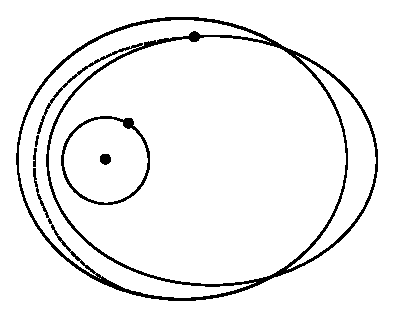
\includegraphics[width=7cm]{Ellipse.eps}
  \end{center}
  \caption{Transition from the osculating ellipse of eccentricty
    $e=0.48$ to the ellipse of eccentricty $e=0.67$. The dashed line
    schematically shows the transition. Nevertheless, the actual
    diffusing orbit is very complicated and diffusion is very slow.}
  \label{fig:EllipseChange}
\end{figure}

In Theorem \ref{MainTheorem:Intro}, we do not know what would happen
asymptotically if we let $\mu\rightarrow 0$ (our estimates worsen).
On the other hand, Theorem \ref{MainTheorem:Intro} holds for realistic
values of $\mu$, which is out of reach of many qualitative results of
perturbation theory where parameters are conveniently assumed to be as
small as needed.

\subsection{Mechanisms of instability}

The result obtained in Theorem \ref{MainTheorem:Intro} gives an
example of large instability for this mechanical system. It can be
interpreted as an example of Arnold diffusion (see \cite{Arnold64}).
Nevertheless, Arnold diffusion usually refers to nearly integrable
systems whereas Hamiltonian \eqref{def:Ham:Cartesian} cannot be
considered as close to integrable since $\mu=10^{-3}$ is fixed. The
mechanism of diffusion used in this paper is somewhat similar to the
so-called Mather problem
(\cite{Mather96,BolotinT99,DelshamsLS00,Kaloshin03}).  This analogy
will be specified in Section \ref{sec:Circular:Outer}.

Arguably, the main source of the existence of instabilities are
\emph{resonances}.  One of the most natural resonances in the
elliptic problem (even a three-body problem) is the \emph{mean motion
  orbital resonances}\footnote{The mean motions are the frequencies of
  the Keplerian revolution of Jupiter and the Asteroid around the Sun: in our case
  the Asteroid makes one full revolution while Jupiter makes seven revolutions.}.  Along such a resonance, Jupiter and the
Asteroid will regularly be in the same relative position. Over a long
time interval, Jupiter's influence could thus a priori pile up and,
despite its small amplitude due to the small mass of Jupiter, could
modify the eccentricity of the Asteroid, instead of averaging out.
According to third Kepler's Law, these resonances take place when
$a^{3/2}$ is close to a rational, where $a$ is the semi major axis of
instant ellipse of the Asteroid.  In our case we consider
\emph{$a^{3/2}$ close to 7}. This resonance is convenient for the
proof.  Nevertheless, one should expect that the same mechanism takes
place for a large number of mean motion orbital resonances.

The semi major axis $a$ and the eccentricity $e$ describe completely
an instant ellipse of the Asteroid (up to orientation).  Therefore,
geometrically Theorem \ref{MainTheorem:Intro} says that the Asteroid
evolves from a Keplerian ellipse of eccentricity $e=0.48$ to one of
eccentricity $e=0.67$, without changing much its semi major axis (see
Figure \ref{fig:EllipseChange}).  In Figure \ref{fig:a-e:diffusion} we
consider the plane $(a,e)$, which describe the ellipse of the
Asteroid.  Then diffusing orbits given by Theorem
\ref{MainTheorem:Intro} correspond to a nearly horizontal line.

\begin{figure}[h]
  \begin{center}
    \psfrag{a}{$a$}\psfrag{e}{$e$}\psfrag{1}{$1$}\psfrag{0}{$0$}
    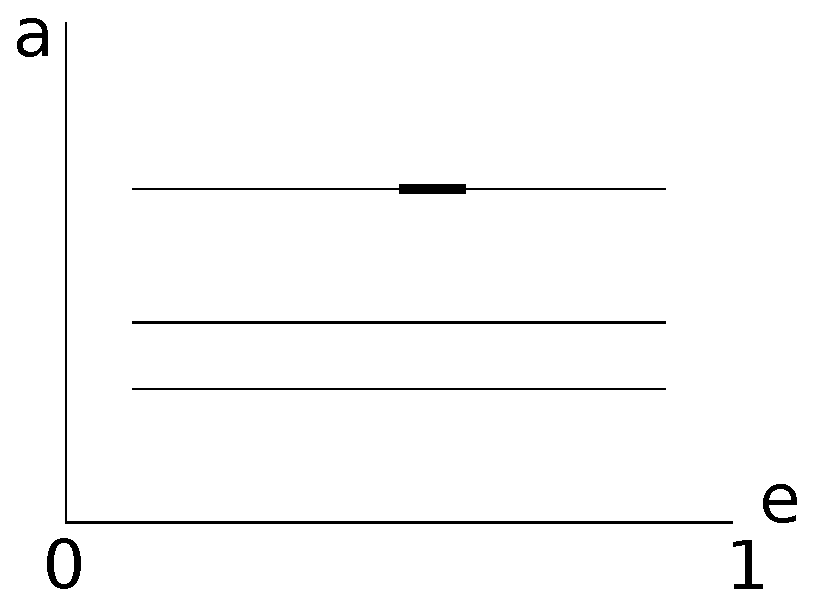
\includegraphics[width=7cm]{Graphae.eps}
  \end{center}
  \caption{In this graphic we show the diffusion path that we study in
    the $(a,e)$ plane.  The horizontal lines represent the resonances
    along which we drift. The thicker line is the diffusion path whose
    existence we are able to prove in this paper.}
  \label{fig:a-e:diffusion}
\end{figure}

\subsection{Presence of instabilities in the Asteroid belt: The Kirkwood gaps}


\subsubsection{The Asteroid belt} One place in the Solar system where
one can apply the dynamics of this problem is the Asteroid belt. 
The Asteroid belt is located  between the orbits of Mars and Jupiter and it consists 
of 1.7 millions of objects ranging from  asteroids of $950$ kilometers size to  dust particles.  Taking into account that the mass 
of Jupiter is approximately 2960 masses of Mars, away from encounters with Mars,
dynamics of Asteroids is well approximated by the Restricted problem. 

Denote by $\mu=m_1/(m_0+m_1)$ the mass ratio. For $\mu=0$ (namely, neglecting Jupiter influence) bounded orbits 
of the Asteroids are ellipses. Up to orientation they are characterized by 
their semimajor axis $a$ and eccentricity $e$. 

A famous result of Lagrange \cite{ArnoldKN88} says that, for $\mu>0$ small, $|a(t)-a(0)|\lesssim \mu$ 
for all $|t|\lesssim 1/\mu$. Niederman shows that well away from 
collisions time estimate can be improved to ...

Nevertheless, if one looks at the Asteroid distribution in terms of the semimajor axis of the osculating ellipse, one encounters several gaps, which are called \emph{Kirkwood gaps}. It is believed that the existence of these gaps is due to instability mechanisms.

\subsubsection{Kirkwood gaps and Wisdom's ejection mechanism}

Call {\it mean motion resonance} when ratio of period of Jupiter 
and period of Asteroid is rational. Then, the Kirkwood gaps correspond to  the ratios $1:3,\ 2:5,\ 3:7$. 
Here we present an heuristic explanation of this phenomenon. 


It is conjectured and confirmed by numerical data \cite{Wisdom82},
that eccentricity of Asteroids placed in the Kirkwood gaps changes by a magnitude of order of one.
Notice that in the real data (see Figure ...) eccentricity
of most Asteroids in the Asteroid belt is between $0$ and $0.18$. 


As eccentricity of Asteroid changes its perihelion $a(1-e)$ gets closer 
and closer to the origin (see figure ...). In particular, Asteroid starts 
to have close encounters with orbits of Mars. Eventually Mars and 
Asteroid come close and Asteroid gets ejected from the Asteroid belt.  

What is surprising is that the change of eccentricity of Asteroid is only
possible to elliptic motions of Jupiter. Indeed, for circular motions of 
Jupiter the problem becomes of two degrees of freedom and there are 
invariant two-dimensional tori separating energy surfaces. 

Heuristically the main conclusion is that if eccentricity of Asteroid
changes by a magnitude of order of one under the Restricted problem
Sun-Jupiter-Asteroid, then the Asteroid might come into zones where 
the Restricted problem does not describe dynamics well. 

The main result of the paper is that in a certain mean motion  
resonance there are unstable motions. In this paper, since the proof relies on numerical computations, we only present results for one particular resonance, but we are confident that this mechanism of instability applies to other 
resonances as long as orbits of unperturbed problem stay away from
collisions. Thus, the instability mechanism showed in this paper gives a possible reason of the existence of the Kirkwood gaps. Another instability mechanism using the adiabatic invariant theory, can be seen in \cite{NeishtadtS04}.





\subsection{Main steps of the proof}

The diffusing orbit of the elliptic problem we are looking for lies
%M,rephrase
%in a neighborhood of a normally hyperbolic invariant cylinder $\Lambda$,
%which is defined by the resonance.
in a neighborhood of a ($3$-dimensional) normally hyperbolic invariant
cylinder $\Lb$ and its local invariant manifolds, which exist near
our mean motion resonance. The vertical component of the cylinder can be
parameterized by the eccentricity of the Asteroid and the horizontal
ones by its mean longitude and time.

If the stable and unstable invariant manifolds of $\Lambda$ intersect
transversally, the elliptic problem induces two different dynamics
on the cylinder (see Sections \ref{sec:CylinderExpansion}
and \ref{sec:Ell:Outer}): {\it the inner and the outer ones}.  The
inner dynamics is simply the restriction of the Newtonian flow to
$\Lambda$.  The outer dynamics is obtained by a limiting process: it
can be observed asymptotically by starting very close to the
cylinder and to its unstable manifold, traveling all the way up to
a homoclinic intersection, and coming back close to the cylinder and
along its stable manifold. Since the system has different homoclinic
orbits to the cylinder, one can define several different outer dynamics.
In our diffusing mechanism we use two different outer maps. The reason
is that each of the outer maps are not defined in the whole cylinder
and then we need the two of them to achieve diffusion (see Section \ref{Section:Circular}).

The proof consists in the following four steps:
%M, remove two `the'. I believe it is correct
\begin{enumerate}
\item Prove existence of the normally hyperbolic invariant
  cylinder $\Lambda$.
\item Establish transversality of the stable and unstable
  invariant manifolds of this cylinder.
\item Compare the inner and outer dynamics on $\Lambda$ and,  in
  particular,  check that they do not have common invariant circles.
\item Construct diffusing orbits by shadowing a carefully chosen
  composition of the outer and inner maps.
\end{enumerate}
This program faces difficulties at every step.
%M, add subsection

\subsubsection{Existence of the normally hyperbolic invariant cylinder $\Lambda$.}
The first difficulty comes
from the proper degeneracy of the Newtonian potential: at the limit
$\mu=0$ (no Jupiter), the Asteroid has a one-frequency, Keplerian
motion, whereas symplectic geometry would allow for a three-frequency
motion (as with any potential other than the Newtonian potential $1/r$
and the elastic potential $r^2$). Due to this degeneracy, switching to
$\mu>0$ is a singular perturbation. In particular, hyperbolicity is
small with respect to $\mu$.

\subsubsection{Transversal of the stable and unstable
  invariant manifolds of the cylinder $\Lambda$.}
The second step, establishing the transversality of the invariant
manifolds of $\Lambda$ is a delicate problem. Asymptotically when
$\mu\ll 1$, the difference between the invariant manifolds becomes
exponentially small with respect to $\mu$, that is of order
$\exp(-c/\sqrt{\mu})$ for some constant $c>0$. Despite inordinate
efforts of splitting specialists, all the known techniques fail here,
because the relevant Poincar{\'e}-Melnikov integral is not algebraic.
This instability mechanism relies on such precise information on the
flow, that in details it is discontinuous with respect to any
reasonable topology. This step simplifies dramatically in the study of
generic systems.
% the potential (not the original potential, but the perturbing potential
% for computing the Poincar{\'e}-Melnikov integral) is not algebraic, which is crucial
% for existing techniques.

At the expense of creating other difficulties, setting $\mu=10^{-3}$
avoids this splitting problem, since for this value of the parameter
one can see that the splitting of separatrices is not extremely small
and therefore, can be detected by means of a computer with a convincing 
accuracy. Besides, $\mu=10^{-3}$ is a realistic value of the mass ratio
for the Sun-Jupiter model. Since the splitting of the separatrices
varies smoothly with respect to the eccentricity $e_0$ of the
primaries, it suffices to estimate the splitting numerically for
$e_0=0$, i.e. in the circular problem. \emph{This is a key
  point for the numerical computation}, which thus remains relatively
simple. On the other hand, in the following two steps it will be crucial
to have $e_0>0$, without which the KAM tori would separate energy
levels.

Finally, recall that the cylinder $\Lambda$ has two branches 
of both stable and unstable invariant manifolds. In certain 
regions the intersections between one of the branches of 
the stable and unstable  invariant manifolds is tangential, 
which does not allow to define the outer map. Nevertheless,
then one can check that the other two branches intersect 
transversally so that we can define a different outer map. 
Thus, we will combine the two outer maps depending which 
branches of the invariant manifolds intersect transversally.

\subsubsection{Calculation of asymptotic formulas for the outer and
inner maps}
Now we turn to the third step. Using classical perturbation theory 
and the specific properties of the underlying system one can reduce 
the inner and (the two different) outer dynamics to three two-dimensional
symplectic maps of the form
\begin{equation}\label{def:InnerMap:ell:intro}
  \FF_{e_0}^\inn:\left(\begin{array}{c} I\\
      t
    \end{array}\right)\mapsto \left(\begin{array}{l} I+ e_0 \left(A^+(I,\mu)e^{it}+
        A^-(I,\mu)e^{-it}\right)+\OO\left(\mu e_0^2\right)\\
      t+\mu\TTT_0(I,\mu)+\OO(\mu e_0)
    \end{array}\right)
\end{equation}
and
\begin{equation}\label{def:OuterMap:Elliptic:Intro}
  \FF_{e_0}^{\out,\ast}:\left(\begin{array}{c} I\\
      t
    \end{array}\right)\mapsto \left(\begin{array}{l} I+ e_0\left(B^{\ast,+}
        (I,\mu)e^{it}+B^{\ast,-} (I,\mu)e^{-it}\right) +\OO\left(\mu e_0^2\right)\\
      t+\mu\omega^\ast(I,\mu)+\OO(\mu e_0)
    \end{array}\right),\,\,\,\ast=\ff,\bb,
\end{equation}
where $(I,t)$ are conjugate variables which parameterize a certain connected
component of the 3-dimensional normally
hyperbolic invariant cylinder $\Lambda$ intersected with a certain transversal
Poincar{\'e} section and $A^\pm, \TTT_0,B^{\ast,\pm}, \omega^\ast$ are analytic
functions. The superindexes $\ff$ and $\bb$ stand for the forward and bacward
heteroclinic orbits that are used to define the outer maps. The choice of
this notation will be clear later on in Section \ref{Section:Circular}. Note
that these maps are real-analytic and therefore $A^-$ and $B^{\ast,-}$ are
the complex conjugates of $A^+$ and $B^{\ast,+}$ respectively.

\subsubsection{Nondegeneracy implying existence of diffusing orbits}
As we will see in Section \ref{sec:ProofDiffusion}, the existence of
diffusing orbits can be established provided the analytic functions
\[
\KK^{\ast,+}(I,\mu)=B^{\ast,+} \left(I,\mu\right)-
\frac{e^{ i\mu\omega^\ast(I,\mu)}-1}{e^{ i\mu\TTT_0(I,\mu)}-1}A^+ \left( I,\mu\right)
\]
do not vanish for  all $I\in[I_-,I_+]$ for which the  corresponding
outer map is defined. Since $A^\pm$ and $B^{\ast,\pm}$ are complex conjugate,
we do not write the complex conjugate $\KK^{j,-}(I,\mu)$.
% \[
% \KK^-(I)=\Omega^- \left(I\right)-\frac{e^{- i\omega_0(I)}-1}{e^{ -i\TTT_0(I)}-1}A^- \left( I\right),
% \] satisfies $\ol{ \KK^-(I)}= \KK^+(I)$, and therefore, both vanish at the same points.
% rephrase
Numerically, one can check that  $\KK^{j,+}(I,\mu)\neq 0$ in their domain
of definition. It turns out that $\KK^{j,+}(I,\mu)\neq 0$ implies absence of common
invariant curves for the inner and outer maps. This reduces the proof of Theorem \ref{MainTheorem:Intro}
to shadowing, made in step 4, and thus it leads to the existence 
of diffusing orbits. Moreover, it turns out that for this problem 
{\it no  large gaps} appear. This fact is not so surprising taking
into account that  the elliptic problem has three time scales.

Finally, let us point out that the complex functions  $\KK^{j,+}(I,\mu)$  can be regarded as
a 2-dimensional real-valued function depending analytically on $(I,\mu)$.
If the dependence in $\mu$ is non-trivial, 
%M, add
a complex valued function $\KK^{j,+}(I,\mu)$ does not vanish at 
any point of their domain of definition except for a finite number of $\mu$'s.

%M, add more explanations

% \subsection{We should put a section on further work and other things}
% Here would be the place to put:


% A realistic value for the eccentricity of Jupiter is $e_J=1/20$ whereas Theorem \ref{MainTheorem:Intro} only apply for arbitrarily small $e_0$. Nevertheless, we believe that the mecanism of diffusion exposed in this paper can be still verified for wider ranges in the eccentricity, even if it is more involved since on has to go more careful while using perturbative methods.

% Talk also about time of diffusion are stability of the solar system.




\subsection{Nature of numerics}

In this section we outline which parts of the mechanism are based 
on numerics. 

\begin{itemize}
\item On each $3$-dimensional energy surface the circular problem 
has a well-defined Poincare map $F_J:\Sigma_J \to \Sigma_J$ 
of a $2$-dimensional cylinder $\Sigma_J$ for a range of $J$'s. 
For each $J$ in some interval $[J_-,J_+]$ we establish the existence 
of a saddle periodic orbit $F^7_J(p_J)=p_J$. 
 
\item We show that for all $J\in [J_-,J_+]$ we have 
two transversal intersections of $W^s(p_J)$ and $W^u(p_J)$. Surprisingly (at least to the authors) ``symmetric'' 
intersection points exhibit tangencies for some $J$'s. Nevertheless, since there are two symmetric intersection points, it is rather easy to check the transversality of one of them for each $J\in [J_-,J_+]$.
   
\item Each transversal intersection $q_J$ gives rise to a homoclinic 
orbit, denoted $\gamma_J$. For each $J\in [J_-,J_+]$ we compute 
several Melnikov integrals of certain quantities related to 
$\Delta H_{\text ell}$ along $\gamma_J$ and $p_J$. Out of these 
integrals we compute the leading terms of the dynamics of the elliptic problem and 
verify a necessary condition for diffusion. 
\end{itemize}
At no point of numerics we study rely on numerics which 
is anywhere close to error of calculations.  
PAU, AQUESTA FRASE S'HA DE CANVIAR.


\section{Setting of the problem and
  notations}\label{sec:SettingsAndResults}

The model of the Sun, Jupiter and a massless Asteroid in cartesian coordinates
is given by the Hamiltonian \eqref{def:Ham:Cartesian}. First, let us consider
the case $\mu=0$, that is, we consider Jupiter with zero mass. In that case,
Jupiter and Asteroid do not make influence on each other and therefore
the system is reduced to two uncoupled 2-body problems, the Sun-Jupiter and
the Sun-Asteroid, which are integrable.

We want to study the existence of instability in one particular
resonance of this system, which appears when the period of Asteroid is
seven times the period of Jupiter. One can consider the so-called
Delaunay variables, which we denote by $(\ell, L, \g, G)$, which are
angle-action coordinates of the Sun-Asteroid system. The variable
$\ell$ is the mean anomaly, $L$ is the square of the semi major axis,
$\g$ is the argument of the perihelion and $G$ is the angular
momentum. These variables can be obtained from the Cartesian
coordinates as follows (see~\cite{ArnoldKN88} for more details and
background, or~\cite[Appendix]{Fejoz:2010} for a straightforward
definition). First define polar coordinates for the position:
\[
q=(r\cos\phi,r\sin\phi).
\]
Then, the actions of Delaunay coordinates are defined implicitly by
\begin{align}
  -\frac{1}{2L^2}&=\frac{\|p\|^2}{2}-\frac{1}{\|q\|}\label{def:L}\\
  G&=-J-\frac{1}{2L^2}\label{def:G}
\end{align}
(recall that $\mu=0$ for these definitions). Using these actions, the
eccentricity of Asteroid can be expressed as
\begin{equation}\label{def:eccentricity}
  e=\sqrt{1-\frac{G^2}{L^2}}.
\end{equation}
To define the angles, let $v$ and $\hat g$ be the true anomaly and the
argument of the perihelion so that
\begin{equation}\label{def:Angles}
  \phi=v+\g.
\end{equation}
Then, from $v$ one can obtain the eccentric anomaly $u$ using
\begin{equation}
  \tan\frac{v}{2}=\sqrt{\frac{1+e}{1-e}}\tan\frac{u}{2}.
\end{equation}
From the eccentric anomaly, the mean anomaly is given by the Kepler equation
\begin{equation}\label{def:MeanAnomaly}
  u-e\sin u=\ell.
\end{equation}

In the Delaunay coordinates, the Hamiltonian \eqref{def:Ham:Cartesian}
can be split into the Keplerian part $-1/2L^2$, the circular part of
the perturbing function $\mu \Delta H_{circ}$ and the remainder which
vanishes when $e_0=0$:
\begin{equation}\label{def:HamDelaunayNonRot}
  \hat H(L,\ell,G, \g,t)=-\frac{1}{2L^2}+\mu\Delta H_\ccirc(L,\ell,G,
  \g-t,t,\mu)+ \mu e_0\Delta H_\eell(L,\ell,G, \g-t,t,\mu,e_0).
\end{equation}
It turns out that for $e_0=0$, the circular problem only depends on
$\g-t$. To simplify the comparison with the circular problem, we
consider rotating Delaunay coordinates, in which $\Delta H_\ccirc$ is
autonomous. This means to define the new angle $g=\g -t$ and a new
variable $I$ conjugate to time $t$. Then, we have
\begin{equation}\label{def:HamDelaunayRot}
  H(L,\ell,G, g,I,t)=-\frac{1}{2L^2}-G+\mu\Delta H_\ccirc(L,\ell,G, g,\mu)+
  \mu e_0 \Delta H_\eell(L,\ell,G, g,t,\mu,e_0)+I.
\end{equation}
In these new variables, the difference of number of degrees of freedom
of the elliptic and circular problems becomes more apparent. When
$e_0=0$ the system is autonomous and then $I$ is constant, which
corresponds to the conservation of the Jacobi constant
(\ref{def:Jacobi}). Therefore, the circular problem reduces to 2
degrees of freedom. Moreover, it will later be crucial to see the
circular problem as an approximation of the elliptic one, in order to
reduce the Herculean (and doubtful) numerical computations of a direct
approach to the corresponding lower dimensional, and thus simpler, computations of the circular
problem.

Recall that we consider the $1:7$ mean motion orbit resonance 
between Jupiter and Asteroid. That is, the period of Asteroid
being approximately seven times the period of Jupiter.
In rotating Delaunay variables, this corresponds to
\begin{equation}\label{def:Resonance}
\dot\ell \sim \frac{1}{7}\quad\text{ and }\quad\dot g\sim -1.
\end{equation}
A nearby resonance is
\[
\dot\ell \sim \frac{1}{7}\quad\text{ and }\quad\dot t\sim 1,
\]
but we will stick to the previous one.

The resonance takes place when $L\sim 7^{1/3}$. We will study 
the dynamics in a large neighborhood of this resonance and 
we will see that one can drift along it. Namely, we will find 
trajectories that keep $L$ close to $7^{1/3}$ while 
the $G$-component changes noticeably. Using \eqref{def:eccentricity}, 
one can see that $e$ also changes by an order of one. 
In this setting, Theorem \ref{MainTheorem:Intro} can be
rephrased as follows.
\begin{theorem}\label{th:MainTheorem:detail}
  There exist $e_0^\ast>0$ such that for $0<e_0<e_0^\ast$, there exist
  $T>0$ and an orbit of the Hamiltonian System with Hamiltonian
  \eqref{def:HamDelaunayRot} which satisfies
  % that is redundant
  \[
  G(0)<G_0\text{ and }G(T)>G_1
  \]
  whereas
  \[
  \left| L(t)-7^{1/3}\right|\leq 7\mu,
  \]
\end{theorem}

% SOMEWHERE: Heuristically, if Jupiter has a not so small eccentricity, diffusion should be
% faster, and paradoxically it is more difficult to detect because
% non-integrability prevents motions from being regular on a small time
% scale.

By definition the Hamiltonian \eqref{def:HamDelaunayRot} is autonomous 
and thus preserved. Therefore, we will
restrict ourselves to a level of energy which, without loss of generality, can
be taken as $H=0$. Therefore,  since $|I-G|=\OO(\mu)$, for orbits satisfying
$\left| L(t)-7^{1/3}\right|\leq 7\mu$, drift in $G$ is equivalent to
drift in $I$.


The proof of this theorem is structured as follows.

In Section \ref{Section:Circular}, we study the dynamics in the circular problem,
that is
% the Hamiltonian System \ref{def:HamDelaunayRot} with $e_0=0$.
% rephrase
$e_0=0$ and the underlying Hamiltonian \eqref{def:HamDelaunayRot} becomes
\begin{equation}\label{def:HamDelaunayCirc}
  H_\ccirc(L,\ell,G, g)=-\frac{1}{2L^2}-G+\mu \Delta H_\ccirc(L,\ell,G, g,\mu).
\end{equation}
{\it Theorem} \ref{th:NHIMCircular} says that for an interval of Jacobi energies
$[J_-,J_+]$ the circular problem has a smooth family of hyperbolic periodic
orbits $\lb_J$,  whose stable and unstable manifolds intersect
transversally for each $J \in [J_-,J_+]$. This theorem implies
(Corollary \ref{coro:NHIMCircular}) existence of a normally hyperbolic
invariant cylinder. Later in the section (Subsections \ref{sec:Circular:Inner}
and \ref{sec:Circular:Outer}) we calculate  the aforementioned circular outer
and inner maps for the circular problem (see \eqref{def:InnerMap:ell:intro} 
and \eqref{def:OuterMap:Elliptic:Intro}).


Then in Section \ref{sec:Elliptic}  we consider the elliptic case $e_0>0$
as a perturbation of the circular case.

{\it Theorem} \ref{th:Elliptic:NHIM} says that the family of periodic orbits
$\{\la_J\}_{J\in [J_-.J_+]}$ give rise to a normally hyperbolic invariant
cylinder $\Lambda_{e_0}$ whose stable and unstable manifolds intersect
transversally for each $J \in [J_-+\delta,J_+ - \delta]$ with small $\delta>0$.
These objects give rise to the inner and outer maps.
{\it Theorem} \ref{th:InnerAndOuter:Elliptic} provides expansions for
the inner and outer maps (see formulas (\ref{def:InnerMap:ell:th}) and
(\ref{def:OuterMap:Elliptic:th}) respectively).

Finally, in Section \ref{sec:ProofDiffusion} in {\it Theorem}
\ref{th:Transition} we complete the proof of Theorem
\ref{th:MainTheorem:detail}. This is done by comparing the inner and 
the two outer maps in Lemma \ref{lemma:Averaging} and constructing a
transition chain of tori.  It turns out that there are {\bf no large gaps}, 
due to the specific structure of times scales and the Fourier series involved. 
This a priori contrasts with the typical situation of
dynamics near a resonance (see e.g. \cite{DelshamsLS06a}).

\begin{notation}
  From now on, we will omit the dependence on $\mu$ (keeping in mind
  at various points the question of what would happen if we let $\mu$
  vary). Recall that we are taking a realistic value of $\mu=10^{-3}$.
\end{notation}

\section{The circular problem}\label{Section:Circular}

The circular problem is given by the Hamiltonian
\eqref{def:HamDelaunayRot} with $e_0=0$.  Since it does not depend on
$t$, $I$ is an integral of motion. Moreover, since we are studying the
dynamics in the energy surface $H=0$, we have $I=-H_\ccirc(\ell,L,g,G)$.
Therefore, the variable $I$ equals the opposite of the Jacobi constant \eqref{def:Jacobi}. For each level
$I=\text{constant}$, one can study the dynamics close to the resonance
$7\dot \ell+\dot g\sim 0$. Since $t$ is a cyclic variable, one can consider
the two degree of freedom Hamiltonian of the circular problem
for which the conservation of energy corresponds to the conservation of
the Jacobi constant \eqref{def:Jacobi}. Moreover, one can see that
the circular problem is reversible with respect to the involution
\begin{equation}\label{def:involution}
 \Psi(L,\ell,G, g,I,t)=(L,-\ell,G,-g,I,-t).
\end{equation}
This symmetry will facilitate several numerical computations.


\begin{theorem}\label{th:NHIMCircular}
  Consider the Hamiltonian \eqref{def:HamDelaunayCirc} with
  $\mu=10^{-3}$.  Then, in each energy level $J_-\leq J\leq J_+$,
  there exists a hyperbolic periodic orbit $\lb_J=(L_J(t), \ell_J(t),
  G_J(t), g_J(t))$ of period $T_J$ which satisfies
  \[
  \left| T_J-14\pi\right|<60 \mu,
  \]
  smooth in $J$, and
  \[
  \left| L_J(t)-7^{1/3}\right|< 7\mu
  \]
  for certain constant $C>0$ and all $t\in\RR$.

  Each $\lb_J$ has two branches of stable and 
  unstable invariant manifolds $W^{s,j}(\lb_J)$ 
  and $W^{u,j}(\lb_J)$, $j=1,2$. Then, for each
  $J\in [J_-,J_+]$ either $W^{s,1}(\lb_J)$ and 
  $W^{u,1}(\lb_J)$ or $W^{s,2}(\lb_J)$ and 
  $W^{u,2}(\lb_J)$ intersect transversally.
\end{theorem}

\begin{proof}
  Based on convincing numerical data. See
  Appendix~\ref{app:NHIMCircular}.
\end{proof}


We will study the elliptic problem as a perturbation of the circular
one.  Therefore we do not reduce the dimension of the phase space
while studying the inner and outer dynamics of the circular
problem. Namely, we consider the \emph{Extended Circular Problem}
given by the Hamiltonian \eqref{def:HamDelaunayRot} with $e_0=0$. In
other words, we keep the conjugate variables $(I,t)$ even if $t$ is a
cyclic variable. Consider the energy level $H=0$.  In this setting the
conservation of the Jacobi constant corresponds to the conservation of
$I$. Therefore, the periodic orbits obtained in Theorem
\ref{th:NHIMCircular} become invariant two-dimensional tori which
belong to hyperplanes $I=\text{constant}$ for any $I\in [I_-,I_+]=
[-J_+,-J_-]$. Moreover, the union of these 2-dimensional invariant
tori form a normally hyperbolic invariant $3$-dimensional manifold.


\begin{corollary}\label{coro:NHIMCircular}
  The Hamiltonian \eqref{def:HamDelaunayRot} with $\mu=10^{-3}$ and
  $e_0=0$ has an analytic normally hyperbolic invariant  $3$-dimensional
  manifold $\Lambda_0$, which is foliated by two-dimensional invariant
  tori.


  Moreover, $\Lambda_0$ has two branches of stable and unstable 
  invariant manifolds, which we call $W^{s,j}(\Lambda_0)$ and 
  $W^{u,j}(\Lambda_0)$, $j=1,2$. Then, in the invariant planes 
  $I=\text{constant}$,  for each $I\in [I_-,I_+]$ either 
  $W^{s,1}(\Lambda_0)$ and $W^{u,1}(\Lambda_0)$ or 
  $W^{s,2}(\Lambda_0)$ and $W^{u,2}(\Lambda_0)$ intersect transversally.
\end{corollary}

% As we have explained in Section \ref{sec:Intro}, the Circular Problem induces the so-called \emph{inner} and \emph{outer} dynamics  in the normally hyperbolic cylinder $\Lambda_0$. We will see that due to the conservation of both the energy and $I$, both dynamics are integrable. To study them  is more convenient to look for

We define a global Poincar{\'e} section and deal with maps to reduce the
dimension by one.  There are two natural choices: $\{t=0\}$ and
$\{g=0\}$, since both variables satisfy $\dot t\neq 0$ and $\dot g\neq
0$.  We choose the section $\{g=0\}$ and call
\begin{equation}\label{def:PoincareMap}
  \PP_0:\{g=0\}\longrightarrow \{g=0\}
\end{equation}
this Poincar{\'e} map. Since we are studying the resonance \eqref{def:Resonance}, the intersection of the cylinder $\Lambda_0$ with the section $\{g=0\}$ is formed by seven cylinders (see Figure \ref{fig:PoincareSection}). We denote them by $\wt \Lambda_0^j$, $j=0,\ldots, 6$. Namely,
\begin{equation}\label{def:Cylinder:Poincare}
\Lambda_0\cap \{g=0\}=\wt\Lambda_0=\cup_{j=0}^6\wt\Lambda_0^j.
\end{equation}
As a whole $\cup_{j=0}^6\wt\Lambda_0^j$ is a normally hyperbolic invariant manifold for the Poincar{\'e} map
$\PP_0$. One can also consider the Poincar\'e map $\PP_0^7$, namely iterate seven times $\PP_0$. Then, for this map, each $\wt\Lambda_0^j$ is a normally hyperbolic invariant manifold (of course, their union is also a normally hyperbolic invariant manifold for $\PP_0^7$). We work with the cylinders $\wt\Lambda_0^j$ since they have the advantage of having a natural system of coordinates. This system of coordinates will be used later on to study the inner and outer dynamics on them. In particular, we will work with $\wt \Lambda_0^3$ and $\wt\Lambda_0^4$. The reason is that in each invariant plane $I=\text{constant}$ they are connected by at least one heteroclinic connection (of $\PP_0^7$) which is symmetric with respect to the involution \eqref{def:involution}. We  call it a forward  heteroclinic orbit if it is asymptotic to $\wt \Lambda_0^3$ in the past and $\wt\Lambda_0^4$ in the future and a backward heteroclinic orbit if it is asymptotic to $\wt \Lambda_0^4$ in the past and to $\wt\Lambda_0^3$ in the future. We denote by $\DD^{\ff} \subset  [I_-,I_+]$, where $\ff$ stands for forward, the subset of $[I_-,I_+]$ where  $W^u(\wt \Lambda_0^3)$ and $W^s(\wt \Lambda_0^4)$ intersect transversally and by $\DD^{\bb} \subset  [I_-,I_+]$, where $\bb$ stands for backward, the subset of $[I_-,I_+]$ where  $W^s(\wt \Lambda_0^3)$ and $W^u(\wt \Lambda_0^4)$ intersect transversally.  By Corollary \ref{coro:NHIMCircular} we have that $\DD^\ff\cup\DD^\bb=  [I_-,I_+]$.


\begin{figure}[h]
  \begin{center}
    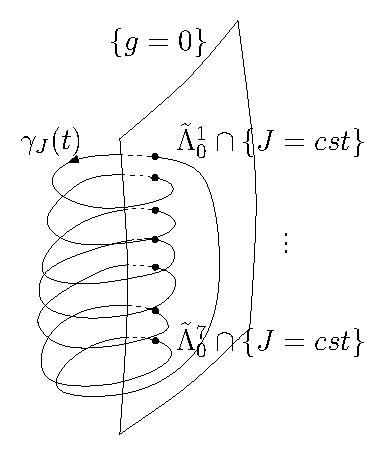
\includegraphics[width=5cm]{gammaJ.eps}
  \end{center}
  \caption{The periodic orbit obtained at each energy level intersects seven times the Poincar\'e section $\{g=0\}$, as it is shown schematically in this picture. Then, when one considers the Poincar\'e map $\PP_0$, the normally hyperbolic invariant manifold $\wt\Lambda_0$ has seven connected components $\wt\Lambda^0_0, \ldots, \wt\Lambda_0^6$.}
  \label{fig:PoincareSection}
\end{figure}



\begin{corollary}\label{coro:NHIMCircular:Poincare}
  The Poincar\'e map $\PP^7_0$ defined in \eqref{def:PoincareMap}, which is 
  induced by the Hamiltonian \eqref{def:HamDelaunayRot} with $\mu=10^{-3}$ 
  and  $e_0=0$, has seven analytic normally hyperbolic invariant manifolds
  $\wt\Lambda_0^j$, $j=0,\ldots,6$. They are foliated by one-dimensional 
  invariant curves. Moreover, there exist analytic functions 
  $\GG^j_0: [I_-,I_+]\times\TT\rightarrow (\RR \times \TT)^3$ which can
  be expressed in coordinates as
  \begin{equation}\label{def:NHIM:Param0}
    \GG_0^j(I,t)=\left(\wt
      \GG_0^j(I),0,I,t\right)=\left(\GG_0^{j,L}(I),\GG_0^{j,\ell}(I),
      \GG_0^{j,G}(I),0,I,t\right),
  \end{equation}
  that parameterize $\wt \Lambda_0^j$, namely,
  \[
  \wt\Lambda^j_0=\left\{ \GG_0^j(I,t):(I,t)\in[I_-,I_+]\times \TT\right\}.
  \]
  The manifolds $W^{u}(\wt\Lambda^3_0)$ and $W^{s}(\wt\Lambda^4_0)$ 
  intersect transversally  provided $I\in \DD^\ff$  and  $W^{s}(\wt\Lambda^3_0)$ 
  and $W^{u}(\wt\Lambda^4_0)$ intersect transversally provided $I\in \DD^\bb$. 
  Moreover, one of the points of these intersections belong to the symmetry axis 
  of \eqref{def:involution}. Let us denote by $\Gamma^{\ast}_0$, $\ast=\ff,\bb$, these
  intersections. Then, there exist functions
  \[
  \CCC^{*}_0: \DD^j\times\RR\rightarrow
  \left(\RR\times\TT\right)^3, \quad (I,t) \mapsto \CCC^*_0(I,t),\,\,\,\ast=\ff,\bb\]
  which parameterize them:
  \[
  \Gamma^*_0=\left\{ \CCC^*_0(I,t)=(\CCC_0^{*,L}(I),\CCC_0^{*,\ell}(I),
    \CCC_0^{*,G}(I),0,I,t):(I,t)\in \DD^\ast\times\TT\right\},\,\,\,\ast=\ff,\bb.
  \]
\end{corollary}

The $0$ that appears in  the parameterizations $\GG$ and $\CCC$ is just the $g$-coordinate. We keep it although we are in the Poincar\'e section because later on we will use these parameterizations in the full phase space. Corollary \ref{coro:NHIMCircular} gives  global coordinates $(I,t)$ for each cylinder $\wt\Lambda^j_0$. These coordinates are symplectic with respect to the canonical symplectic form
\begin{equation}\label{def:InnerDiffForm}
 \Omega_0=dI\wedge dt,
\end{equation}
Indeed, one has to consider the pullback of the canonical form $dL\wedge d\ell+dG\wedge dg+dI\wedge dt$ to the cylinders $\wt\Lambda_0^j$. By Corollary \ref{coro:NHIMCircular:Poincare} we have that in the cylinders: $g=0$, $\ell=\GG_0^{j,\ell}(I)$ and $L=\GG_0^{j,L}(I)$. Then, it is easy to see that the pullback of $dL\wedge d\ell+dG\wedge dg+dI\wedge dt$ is just $\Omega_0$.


We consider the inner and the two outer maps in one of these cylinders. We choose $\wt\Lambda_0^3$. As we have explained before, the reason is that their heteroclinic connections with the following cylinder $\wt\Lambda_0^4$ intersect the symmetry axis of the involution \eqref{def:involution} and therefore they are easier to be studied numerically (see Figure ??). Since $I$ is conserved by the inner and outer maps, these maps are integrable and the variables $(I,t)$ are the action-angle variables. In this way, it will be easier
to understand the influence of the ellipticity.


\subsection{The inner map of the circular problem}\label{sec:Circular:Inner}
We first obtain the inner map. One could define it as the Poincar\'e map $\PP_0$ restricted to the whole normally hyperbolic invariant manifold \eqref{def:Cylinder:Poincare}. Nevertheless, to study the diffusion mechanism it is more convenient to consider just one of the cylinders that form \eqref{def:Cylinder:Poincare}, for instance $\wt\Lambda_0^3$. To this end, we can define the inner map $\FF_0^\inn:\wt\Lambda_0^3 \rightarrow \wt\Lambda_0^3$ as the Poincar\'e map $\PP^7_0$ restricted to $\wt\Lambda_0^3$, which leaves it invariant. We use the global coordinates $(I,t)$ of $\wt\Lambda_0^3$ to express it.

Since
$I$ is an integral of motion, this inner map is of the form
\begin{equation}\label{def:InnerMap:Circular}
  \FF_0^\inn:\left(\begin{array}{c} I\\
      t
    \end{array}\right)\mapsto \left(\begin{array}{c} I\\
      t+\mu\TTT_0(I)
    \end{array}\right),
\end{equation}
where the function $\TTT_0$ is independent of $t$ due to the fact that
the inner map preserves the differential form \eqref{def:InnerDiffForm}, which does not depend on $t$, and that $I$ is a first integral.  In fact, $14\pi+\mu\TTT_0(I)$ is the period of
the periodic orbit obtained in Theorem \ref{th:NHIMCircular} on the
corresponding energy surface. It can be seen numerically that this map
is twist.

\begin{lemma}\label{lem:TwistInner}
  The inner map $\FF_0^\inn$ defined in \eqref{def:InnerMap:Circular}
  is a symplectic twist map, that is
  \[
  \pa_I \TTT_0(I)\neq 0\qquad \text{for }I\in [I_-,I_+].
  \]
  Moreover, the function $\TTT_0(I)$ satisfies
  \begin{equation}\label{eq:IntervalTwist}
    0<\mu\TTT_0(I)<\pi.
  \end{equation}
\end{lemma}

\begin{proof}
  Based on convincing numerical data. See Appendix \ref{app:NHIMCircular}.
\end{proof}

In Section \ref{sec:Circular:Outer}, the function $\TTT_0(I)$ will be
written by means of an integral (see \eqref{def:T0:Integral}).

The information contained in this lemma will be crucial in Section \ref{sec:ProofDiffusion}
to prove the existence of a transition chain of invariant tori.

\subsection{The outer map of the circular
  problem}\label{sec:Circular:Outer}

The outer map has been also called scattering map (see for instance
\cite{DelshamsLS08}). 
%M, I am not satisfies the way it was defined before. So I write it differently.
In order to define the outer map we use the perturbative structure of the problem. 
Let $\PP_0$ be a map of a compact manifold $M$ endowed with a smooth metric $\rho$. 
Let $\Lambda_0 \subset M$ be a normally hyperbolic invariant manifold of $\PP_0$.
Assume that dynamics on $\Lb_0$ has zero Lyapunov exponents, e.g. for any 
$z\in \Lb_0$ we have $\lim \ln \|dP^n(z)v\|/n = 0$ for any $v\in T_z\Lb_0$.

Assume that an invariant manifold $\Lambda_0$ is normally hyperbolic and its
stable and unstable invariant manifolds intersect transversally. Then,
the outer map is defined as follows\footnote{This definition can be
  modified to generalize the outer map to any normally hyperbolic
  invariant manifold with transversal stable and unstable invariant
  manifolds}.

Since $\Lb_0$ is normally hyperbolic it is persistent under small 
perturbation of $\PP_0$. 

\begin{definition}\label{definition:OuterMap}
%*** CHANGE THE DEFINITION ***
Fix $\lb>1$ and a small perturbation $\PP$ of $\PP_0$.   
Let $\Lambda\subset M$ be a normally hyperbolic invariant 
manifold of $\PP$.  Assume that $\gamma\subset W^s_\Lambda\cap W^u_\Lambda$
is a homoclinic manifold and that the intersection of $W^s_\Lambda$ 
and $W^u_\Lambda$ is transversal along $\gamma$, that is
  \[
  \begin{split}
    T_z W^s_\Lambda+T_z W^u_\Lambda&=T_z M,\quad\text{ for }z\in \gamma\\
    T_z W^s_\Lambda\cap T_z W^u_\Lambda&=T_z\gamma,\quad\text{ for }z\in \gamma.
  \end{split}
  \]
  Then, 
  %there exists a constant $\lambda>1$ such that 
  %for any two points $x_\pm\in\Lambda$  
  we say that $\SSS(x_-)=x_+$, if there exists a point $z\in \gamma$ 
  such that for some $C>0$ we have 
  \[
  \mathrm{dist}\left(\PP^n(z),\PP^n(x_\pm)\right)< C\lambda^{-|n|}\qquad \text{for all }n\in\ZZ^\pm.
  \]
\end{definition}
\begin{remark}
%M, I do not understand remark below so I comment it
%  Even if for a fixed $x_-$, $z$ is not unique, the point $x_+$ is unique. This makes the outer map well defined.
Since $\Lb$ is normally hyperbolic, for each point $x \in \Lb$ 
there are strong stable and unstable manifolds $W^{ss}(x)$ and 
$W^{su}(x)$. Then $\SSS(x_-)=x_+$ holds only if $W^{su}(x_-) \cap W^{ss}(x_+)
\ne \emptyset$ and the intersection occurs on $\gamma$.  Due to smooth 
dependence on initial conditions $\SSS$ is smooth.  

In the case when Lyapunov exponents on inner dynamics $\PP$ are not 
close to one, $\lb$ has to exceed maximal Lyapunov exponent to 
have domination of convergence toward $\Lb$ over motion inside of $\Lb$.
Otherwise, one cannot distinguish if an orbit converges to a point on
a stable manifold of a periodic point of the restriction $P|_\Lb$
or it converges to this periodic point.
\end{remark}

One could apply this definition to the normally hyperbolic invariant 
manifold $\cup_{j=1}^7 \wt\Lambda^j_0$. Nevertheless, since it does not 
have a good global system of coordinates is more convenient to proceed 
as we have done for the inner map in the previous section. Namely, 
we look for an outer map which sends $\wt\Lambda_0^3$ to itself.  Now 
one has to be more careful since one cannot consider the outer maps 
induced by the Poincar\'e map $\PP_0^7$. Indeed, for $\PP_0^7$, 
the cylinder $\wt\Lambda_0^3$ is a normally hyperbolic invariant manifold 
but the homoclinic points obtained in Theorem \ref{coro:NHIMCircular} 
now correspond to heteroclinic connections between $\wt\Lambda_0^3$ and 
$\wt\Lambda_0^4$ and between  $\wt\Lambda_0^4$ and $\wt\Lambda_0^3$. 
To overcome this problem we will compose the heteroclinic outer maps 
$\SSS^{\ast}$, $*=\ff,\bb$ with the Poincar\'e map $\PP_0$ as many times 
as necessary so that the composition goes from $\wt\Lambda_0^3$ to itself.

%Recall that $\ff$ stand for forward, namely the outer map associated to a heteroclinic orbit connecting $\wt\Lambda_0^3$ and $\wt\Lambda_0^4$, and $\bb$ for backward, namely the outer map associated to a heteroclinic orbit connecting $\wt\Lambda_0^4$ and $\wt\Lambda_0^3$.

Therefore, this new outer maps $\FF_0^{\out,\pm}$ that we consider connect $\wt\Lambda_0^3$ to itself and are defined as
\begin{equation}\label{def:OuterCircular:Composition}
 \begin{split}
  \FF_0^{\out,\ff}=\PP_0^6\circ\SSS^\ff: \wt\Lambda_0^3\longrightarrow \wt\Lambda_0^3\\
  \FF_0^{\out,\bb}=\SSS^\bb\circ\PP_0: \wt\Lambda_0^3\longrightarrow \wt\Lambda_0^3
 \end{split}
\end{equation}
where $\SSS^\ff$ is the outer map which connects $\wt\Lambda_0^3$ and $\wt\Lambda_0^4$ through $W^u(\wt\Lambda_0^3)\cap W^s(\wt\Lambda_0^4)$ and $\SSS^\bb$ is the outer map which connects $\wt\Lambda_0^4$ and $\wt\Lambda_0^3$ through $W^u(\wt\Lambda_0^4)\cap W^s(\wt\Lambda_0^3)$. Note that here we are abusing notation since the forward and backwards outer maps are only defined provided $I\in \DD^\ff$ and $I\in\DD^\bb$ respectively and not in the whole cylinder $\wt\Lambda_0^3$.

The outer map is always exact symplectic (see \cite{DelshamsLS08}).
Then in the circular problem, since $I$ is preserved, the outer maps have to be of the form
\begin{equation}\label{def:OuterMap:Circular}
  \FF_0^{\out,\ast}:\left(\begin{array}{c} I\\
      t
    \end{array}\right)\mapsto \left(\begin{array}{c} I\\
      t+\mu\omega^\ast(I)
    \end{array}\right),\,\,\,\ast=\ff,\bb.
\end{equation}
The outer map can be defined either with discrete or continuous time. Since the Poincar{\'e}-Melnikov
theory is considerably simpler for flows than for maps, we compute $\FF^{\out,\ast}_0$ using continuous time.
Moreover, in Section \ref{sec:Ell:Outer} we will use also flows to study
the outer map of the elliptic problem as a perturbation of \eqref{def:OuterMap:Circular}.
The outer map  given by the Hamiltonian  \eqref{def:HamDelaunayRot} with $e_0=0$ does
not preserve the section $\{g=0\}$ but the inner map does. In order to fix this problem,
we reparameterize the flow so that the inner and outer map preserve this section.

% Therefore, we will need a flow, whose associated outer map in $\Lambda_0$ induces an outer map on  $\wt \Lambda_0$ in \eqref{def:Cylinder:Poincare}. To obtain it, it is enough to reparameterize the flow associated to the Hamiltonian \eqref{def:HamDelaunayRot} with $e_0=0$ to identify $g$ with time. By time, here we mean the time of the differential equation, since after reparameterization $t$ cannot be identified as time anymore.

This reparameterization corresponds to identifying the variable $g$ with
time and is given by,
\begin{equation}\label{def:Reduced:ODE:Circ}
  \begin{array}{rlcrl}
    \frac{d}{ds} \ell=&\frac{\pa_L H}{-1+\mu\pa_G\Delta
      H_\ccirc}&\text{   }&\frac{d}{ds} L=&-\frac{\pa_\ell
      H}{-1+\mu\pa_G\Delta H_\ccirc}\\
    \frac{d}{ds} g=&1&\text{   }&\frac{d}{ds} G=&-\frac{\pa_g
      H}{-1+\mu\pa_G\Delta H_\ccirc}\\
    \frac{d}{ds} t=&\frac{1}{-1+\mu\pa_G\Delta H_\ccirc}&\text{
    }&\frac{d}{ds} I=&0
  \end{array}
\end{equation}
where $H$ is Hamiltonian \eqref{def:HamDelaunayRot} with $e_0=0$.
Notice that this reparameterization implies the change of direction of
time.  However, the geometric objects stay the same. In particular,
the new flow still possesses the normally invariant cylinder obtained
in Corollary \ref{coro:NHIMCircular} and its invariant manifolds.

We will refer to this system as a \emph{reduced circular problem}.  We
call it reduced because we identify $g$ with the time $s$. Moreover,
the $t$-component (and in fact, all the others) only depends on the other coordinates. Denote by $\Phi_0^\ccirc$ the flow associated to the $(L,\ell,G,g)$ components of equation \eqref{def:Reduced:ODE:Circ} (which are independent of $t$ and $I$). Componentwise it can be written as
\begin{equation}\label{def:Flow:Circular}
  \Phi^\ccirc_0\{s,(L,\ell,G,g)\} =
  \left(\Phi^L_0\{s,(L,\ell,G,g)\}, \Phi^\ell_0\{s,(L,\ell,G,g)\},
    \Phi^G_0\{s,(L,\ell,G,g)\}, g+s\right).
\end{equation}
Then, the outer map can be computed as follows.

Let
\begin{equation}\label{def:OrbitsForOuterMap}
\begin{split}
\gamma_I^\ast(\sigma) &=
\Phi^\ccirc_0\{\sigma,(\CCC_0^{\ast,L}(I),\CCC_0^{\ast,\ell}(I),\CCC_0^{\ast,G}(I),0)\},\,\,\,\ast=\ff,\bb\\
\gamma_I^j(\sigma) &=
\Phi^\ccirc_0\{\sigma,(\GG_0^{j,L}(I),\GG_0^{j,\ell}(I),\GG_0^{j,G}(I),0)\}\\
\end{split}
\end{equation}
be trajectories of the circular problem. The first ones have the initial conditions at the homoclinic points obtained in Theorem \ref{th:NHIMCircular}
 with action $I$ since $\CCC^{\ff,\bb}_0$ are the parameterizations of
the intersections of the invariant manifolds of $\wt\Lambda_0^3$ and $\wt\Lambda_0^4$, given in
Corollary~\ref{coro:NHIMCircular:Poincare}. The second ones have the initial condition in the fixed points of the Poincar\'e map $\PP_0^7$, which are parameterized by $\GG_0^3$ and $\GG^4_0$ given in Corollary \ref{coro:NHIMCircular:Poincare}.

\begin{lemma}\label{lem:Omega0}
  The functions $\omega^{\ff,\bb}(I)$ involved in the definition of the outer
  maps in \eqref{def:OuterMap:Circular} can be defined as
  \[
  \omega^\ast(I)= \omega^\ast_\out(I)+\omega_\inn^\ast (I),
  \]
where
\begin{equation}\label{def:Omega0:OuterPart}
 \omega^\ast_\out(I)=\omega_+^\ast(I)-\omega^\ast_-(I)
\end{equation}
  with
  \begin{equation}\label{def:Omega0PlusMinus}
 \begin{split}
 \omega_+^\ast(I)&=\lim_{N\rightarrow+\infty}\left(\int_0^{ 14N\pi
      }\frac{(\pa_G\Delta
        H_\ccirc) \circ \gamma_I^\ast(\sigma)}{-1+\mu(\pa_G\Delta
        H_\ccirc) \circ \gamma_I^\ast(\sigma)} \, d\sigma+N\TTT_0(I)\right)\\
\omega^\ast_-(I)&=\lim_{N\rightarrow-\infty}\left(\int_0^{ 14N\pi
      }\frac{(\pa_G\Delta
        H_\ccirc) \circ \gamma_I^\ast(\sigma)}{-1+\mu(\pa_G\Delta
        H_\ccirc) \circ \gamma_I^\ast(\sigma)} \, d\sigma+N\TTT_0(I)\right),\,\,\,\ast=\ff,\bb
\end{split}
\end{equation}
\begin{equation}\label{def:Omega0:InnerPart}
\begin{split}
 \omega_\inn^\ff(I)&=\int_0^{ -12\pi
      }\frac{(\pa_G\Delta
        H_\ccirc) \circ \gamma_I^4(\sigma)}{-1+\mu(\pa_G\Delta
        H_\ccirc) \circ \gamma_I^4(\sigma)} \, d\sigma\\
\omega_\inn^\bb(I)&=\int_0^{ -2\pi
      }\frac{(\pa_G\Delta
        H_\ccirc) \circ \gamma_I^3(\sigma)}{-1+\mu(\pa_G\Delta
        H_\ccirc) \circ \gamma_I^3(\sigma)} \, d\sigma,
\end{split}
\end{equation}
where  $\TTT_0(I)$ is the function in \eqref{def:InnerMap:Circular}.
\end{lemma}

Note that the minus sign that appears in the limits of integration of the
integrals involved in the definition of functions $\omega_\inn^\ast(I)$ is
due to the fact that the reparameterized flow \eqref{def:Reduced:ODE:Circ}
reverses time. Using that the circular problem is symmetric with respect
to \eqref{def:involution} and that the homoclinic points $\CCC_0^{\ff}$
and $\CCC_0^{\bb}$ belong to the symmetry axis, one can easily see that
$\omega^\ast_-=-\omega^\ast_+$, $\ast=\ff,\bb$.

The geometric interpretation of $\omega^{\ff,\bb}(I)$ is that the $t$-shift
occurs since the homoclinic orbits approach different points of the
same invariant curve in the future and in the past. This shift is
equivalent to the shift in $t$ that appears in the Mather Problem
\cite{Mather96}. See, for instance, formula (2.1) in Theorem 2.1 of
\cite{DelshamsLS00} and the constants $a$ and $b$ used in formula
(1.4) of \cite{BolotinT99}.

\begin{proof}
We compute $\omega^\ff(I)$. The other case can be done analogously.
  Since the $t$-component of the reduced circular system \eqref{def:Reduced:ODE:Circ} does not depend on $t$, its behavior is given by
  \begin{equation}\label{eq:Flow:Circ:Time}
    \begin{split}
      \Phi_0^t\{s,(L,\ell,G,g,t)\}&=t+\wt\Phi_0 \{s,(L,\ell,G,g)\}\\
      &=t+\int_0^s \frac{1}{-1+\mu\pa_G\Delta
        H_\ccirc\left(\Phi^\ccirc_0\{\sigma,(L,\ell,G,g)\}\right)} \,
      d\sigma
    \end{split}
  \end{equation}
  Note that, using this flow, the inner map on
  \eqref{def:InnerMap:Circular} is just the $(-14\pi)$-time map in the
  time $s$. Then, the original period of the periodic orbits obtained
  in Theorem \ref{th:NHIMCircular}, can be expressed using this new
  flow as
  \begin{equation}\label{eq:PeriodThroughIntegrals}
    14\pi+\mu\TTT_0(I)=\int_0^{-14\pi}\frac{1}{-1+\mu(\pa_G\Delta
      H_\ccirc) \circ \gamma^3_I(\sigma)} \, d\sigma.
  \end{equation}
  This allows us to define the function $\TTT_0(I)$
  in~\eqref{def:InnerMap:Circular} through integrals as
  \begin{equation}\label{def:T0:Integral}
    \TTT_0(I)=\int_0^{-14\pi} \frac{(\pa_G\Delta H_\ccirc) \circ
      \gamma^3_I(\sigma)}{-1+
      \mu (\pa_G\Delta H_\ccirc) \circ \gamma^3_I(\sigma)} \, d\sigma.
  \end{equation}

  Consider now a point
  $(\CCC_0^{\ff,L}(I),\CCC_0^{\ff,\ell}(I),\CCC_0^{\ff,G}(I),0,I,t)$ in
  $W^u(\wt \Lambda^3_0)\cap W^s(\wt \Lambda^4_0)\cap\{g=0\}$. Since the first
  four components are independent of $t$,
  $(\CCC_0^{\ff,L}(I),\CCC_0^{\ff,\ell}(I),\CCC_0^{\ff,G}(I),0,I,t)$ is forward
  asymptotic (in the reparameterized time) to a point
  \[
  \left(\GG_0^{3,L}(I),\GG_0^{3,\ell}(I),\GG_0^{3,G}(I),0,I,t+\mu\omega_+^\ff(I)\right)
  \]
  and backward asymptotic  (in the reparameterized time) to a
  point \[\left(\GG_0^{4,L}(I),\GG_0^{4,\ell}(I),
    \GG_0^{4,G}(I),0,I,t+\mu\omega_-^\ff(I)\right).\]
  Using~\eqref{eq:Flow:Circ:Time}, the functions $\omega_\pm^\ff(I)$ can
  be defined as
  \begin{equation}\label{def:OmegaSmall}
  \begin{split}
    \omega_+^\ff(I)=\lim_{T\rightarrow+\infty}\int_0^{ T}\Bigg(
    \frac{1}{-1+ \mu (\pa_G\Delta H_\ccirc) \circ \gamma^\ff_I(\sigma)}
    -\frac{1}{-1+\mu (\pa_G\Delta H_\ccirc) \circ
      \gamma^3_I(\sigma)}\Bigg) \, d\sigma\\
\omega_-^\ff(I)=\lim_{T\rightarrow-\infty}\int_0^{ T}\Bigg(
    \frac{1}{-1+ \mu (\pa_G\Delta H_\ccirc) \circ \gamma^\ff_I(\sigma)}
    -\frac{1}{-1+\mu (\pa_G\Delta H_\ccirc) \circ
      \gamma^4_I(\sigma)}\Bigg) \, d\sigma.
\end{split}
\end{equation}
  Moreover, since the system is $14\pi$-periodic in the time $s$ due
  to the identification of $s$ with $g$, it is more convenient to
  write these in integrals as
  \[
\begin{split}
  \omega^\ff_+(I)=\lim_{N\rightarrow+\infty}\int_0^{ 14N\pi
  }\Bigg(\frac{1}{-1+ \mu (\pa_G\Delta H_\ccirc) \circ
    \gamma^\ff_I(\sigma)} -\frac{1}{-1+\mu (\pa_G\Delta H_\ccirc) \circ
    \gamma^3_I(\sigma) }\Bigg) \,d\sigma.\\
  \omega^\ff_-(I)=\lim_{N\rightarrow-\infty}\int_0^{ 14N\pi
  }\Bigg(\frac{1}{-1+ \mu (\pa_G\Delta H_\ccirc) \circ
    \gamma^\ff_I(\sigma)} -\frac{1}{-1+\mu (\pa_G\Delta H_\ccirc) \circ
    \gamma^4_I(\sigma) }\Bigg) \,d\sigma.
\end{split}
 \]
  % The flow \eqref{def:Reduced:ODE:Circ} induces the same inner map \eqref{def:InnerMap:Circular} as the original one but now it can be interpreted as the $14\pi$-Poincar{\'e} map in the $s$-time. Then, the second part of the integral is just the evolution of the $t$-component under the flow restricted to the cylinder $\Lambda_0$. Then, using the inner map defined in \eqref{def:InnerMap:Circular}, the functions $\omega_0^\pm(I)$ can be defined as
  Then, taking~\eqref{eq:PeriodThroughIntegrals} into account, one
  obtains
  \[
    \omega_\pm^\ff(I)=\lim_{N\rightarrow\pm\infty}\Bigg(\int_0^{ 14N\pi }
    \frac{1}{-1+\mu(\pa_G\Delta H_\ccirc) \circ \gamma^\ff_I(\sigma)}\,
    d\sigma+N(14\pi+\TTT_0(I))\Bigg),
  \]
  from which the formulas for $\omega_\pm^\ff$ in \eqref{def:Omega0PlusMinus} follow.

Finally we have to compute $\omega_\inn^\ff(I)$. This term corresponds to the contribution of $\PP^6_0$ to the outer map in formula \eqref{def:OuterCircular:Composition}. Then, taking into account that $t$ is defined modulo $2\pi$ is straightforward to obtain  $\omega_\inn^\ff(I)$ in \eqref{def:Omega0PlusMinus}.
\end{proof}




% Let us point out that $14\pi+\TTT_0(I,\mu)$ in the original time $t$ was just the period of the periodic orbit. Now, it is not the period anymore, but is given by the evolution in the variable $t$, and then it is given by the relation
% \[
% 14\pi+\mu \TTT_0(I)=\int_0^{-14\pi}\frac{1}{-1+\mu\pa_G\Delta H_\ccirc(\ell_p(s,I), L_p(s,I),g_p(s,I),G_p(s,I))}ds
% \]
% where $(\ell_p(s,I), L_p(s,I),g_p(s,I),G_p(s,I))$ is the periodic trajectory in the level of energy $J=-I$. Recall that the %reparameterization of time has changed the orientation of the flow, that is why we are doing all the integrals backwards. Then,
% \[
% \TTT_0(I)= \int_0^{-14\pi}\frac{\pa_G\Delta H_\ccirc(\ell_p(s,I), L_p(s,I),g_p(s,I),G_p(s,I))}{-1+\mu\pa_G\Delta H_\ccirc%(\ell_p(s,I), L_p(s,I),g_p(s,I),G_p(s,I))}ds.
%   \]
%   To express $\pa_G \Delta H_\ccirc$ is not straighforward. That's why we think that it is easier to compute these integrals (and the ones that appear in next sections) using rotating Delaunay coordinates instead of rotating cartesian coordinates. In Section \ref{sec:RotatingToDelaunay}, we explain how to change from one coordinates to the others and we also compute  $\pa_G \Delta H_\ccirc$.




%   Recall that (omiting the dependence on the variables) the ode associated to \eqref{def:FullHam} is given by
%   \[
%   \begin{array}{rlcrl}
%     \dot \ell=&\pa_L H&\text{   }&\dot L=&-\pa_\ell H\\
%     \dot g=&-1+\mu\pa_G\Delta H_\ccirc +\mu e_0\pa_G\Delta H_\eell&\text{   }&\dot G=&-\pa_g H\\
%     \dot t=&1&\text{   }&\dot I=&-\mu e_0\pa_t \Delta H_\eell.
%   \end{array}
%   \]

%   Since we have not modified the phase space (only time), the reduced circular problem has still  the invariant cylinder $\CCC_0$. We use %this new ode to obtain the inner and outer maps, which send $\CCC_0$ to itself. From these maps, we will derive later the inner and %outer maps  for the full elliptic problem using perturbative methods.

%   Let us point out that for the reduced circular problem, the ode restricted to $(\ell,L,g,G)$ does not depend on $t$ (nor $I$). Then, one %can just integrate these four variables, and then use the obtained flow to deduce the evolution of $t$. On the other hand, recall that %for the circular problem $I$ is constant. Moreover, one can just identify $g$ with the time $s$ and then deal with this system as a 3 %dimensional system. That probably makes easier to compute the periodic orbit through a Newton method because you have one degeneracy %less in the differential of the Poincar{\'e} map.



%   \section{The inner and outer dynamics of the circular problem}

%   The outer map has the same form, that is,
%   \begin{equation}\label{def:OuterMap:Circular}
%     \FF_0^\text{out}:\left(\begin{array}{c} I\\
%         t
%       \end{array}\right)\mapsto \left(\begin{array}{c} I\\
%         t+\mu\omega_0(I)
%       \end{array}\right).
%   \end{equation}
%   Here we explain how to compute $\omega_0(I)$. On the other hand, since now the orientation is reversed with respect to the original system, the stable and unstable manifolds that Pau obtained have switched. We obtain $\omega_0(I)$ by the formula
%   \[
%   \omega_0(I)=-\omega_0^-(I)-\omega_0^+(I).
%   \]
%   So now, we are going to describe how to obtain $\omega_0^+(I)$ ($\omega_0^-(I)$ can be done analogously). We are going to explain everything using rotating Delaunay coordinates. There are computations that can be much easily done in Delaunay than in cartesian. Later in Section \ref{sec:RotatingToDelaunay}, we explain how to obtain the rotating Delaunay coordinates from rotating cartesian.

%   Let us fix $(I_0,t_0)$, that is level of energy and initial condition in $t$. Then, we have to consider a homoclinic point \emph{in the middle} of the separatrix belonging to the section $\{g=0\}$. Recall that the homoclinic points that Pau found belonged to the section $\{y=0\}$. The symmetry argument does not apply to the homoclinic orbit, and therefore his point does not belong to $\{g=0\}$. Then, we have to obtain a different homoclinc point, which has coordinates $(\ell_h,L_h,0,G_h)$, close to the one that Pau found. Take then the extended point $(\ell_h,L_h,0,G_h,t_0)$ and iterate it from $s=0$ until $s=14 N\pi$ for certain big natural $N$. We have obtained a new point $(\ell_h^+,L_h^+,0,G_h^+,t_1)$ which is very close to a point on the cylinder with coordinates $(\ell_p,L_p,0,G_p,t_1)$ (the first components $(\ell_p,L_p,0,G_p)$ are just the intersecting point between the corresponding periodic orbit and the section $\{g=0\})$.

%   Since the way Pau has computed things is first to obtain the periodic orbit and from it the homoclinic, I understand that the identification of $(\ell_p,L_p,0,G_p)$ from $(\ell_h^+,L_h^+,0,G_h^+)$ should be easy. On the other hand,  the periodic orbit is symmetric (reversible) with respect to the involution $R(\ell,L,g,G)=(-\ell,L,-g,G)$. This makes that the point in the periodic orbit that Pau finds, which belongs to his Poincar{\'e} section $\{y=0\}$, also belongs to our Poincar{\'e} section $\{g=0\}$. From this fact, one can deduce that this point satisfies $\ell_p=0$.


%   Now we iterate backwards this point $14 N\pi$, that is, from $s=0$ to $s=-14N\pi$, obtaining a new point which have coordinates $(\ell_p,L_p,0,G_p,t_2)$ (recall that the first coordinates are in a periodic orbit). From the definition of the inner map, it is clear that $t_2=t_1+N\mu \TTT_0(I)$. Then, taking into account that we are working all the time modulus $14\pi$, we have that
%   \begin{equation}\label{def:t:shift:circular:outer:plus}
%     \omega^+_0(I)=t_2-t_0=\int_{0}^{14N\pi}\frac{\pa_G\Delta H_\ccirc(\ell_h(s), L_h(s),g_h(s),G_h(s))}{-1+\mu\pa_G\Delta H_\ccirc(\ell_h(s), L_h(s),g_h(s),G_h(s))}ds+N\mu \TTT_0(I)
%   \end{equation}
%   where $(\ell_h(s), L_h(s),g_h(s),G_h(s))$ is the orbit of the reduced circular problem with initial condition $(\ell_h,L_h,0,G_h)$. Recall that all the signs go the inverse way that expected since, with the $s$-time everything is reversed.


%   Analogously, one can define $\omega^-_0(I,\mu)$ as
%   \begin{equation}\label{def:t:shift:circular:outer:minus}
%     \omega^-_0(I)=\int_{-14N\pi}^{0}\frac{\pa_G\Delta H_\ccirc(\ell_h(s), L_h(s),g_h(s),G(s,I))}{-1+\mu\pa_G\Delta H_\ccirc%(\ell_h(s), L_h(s),g_h(s),G_h(s))}ds+N\mu \TTT_0(I).
%     \end{equation}

%     With these computations, we finish the study of the outer map of the circular problem.

%     Then, let us take an initial condition on the periodic orbit intersected with $\{g=0\}$ extended with $t$, that is $(\ell_0,L_0,0,G_0,t_0)$ (which depends on $I$). Then, we iterate this point forward $14 N\pi$ for a big $N$ (how big is $N$ has to be determined...). Then, we obtain a new point which is  $(\ell_0,L_0,0,G_0,t_1)$, that is, the first coordinates are just the same by periodicity but $t$ has changed. In fact, $t_1$ is just $t_1=t_0+\mu N\TTT_0(-I,\mu)$ (recall that we work modulus $14\pi$). Then, consider the point $(\ell_h,L_h,0,G_h,t_1)$, where $(\ell_h,L_h,0,G_h)$ are the coordinates of a point homoclinic to the periodic orbit we are dealing with which belongs to the original local stable invariant manifold (which corresponds to the unstable manifold of the reparameterized system). We choose this point such that is $14 N\pi$ far from the \emph{first} homoclinic point. Then, iterate it backwards during $28N\pi$ of $s$-time to obtain a new point $(\ell_h',L_h',0,G_h',t_2)$. Since we are taking $N$ big, the point $(\ell_h',L_h',0,G_h')$ is again very close to $(\ell_0,L_0,0,G_0)$ and belongs to the local unstable invariant manifold of the original system (local stable invariant manifold of the original one). Now we again iterate forward $14\pi N$ to obtain the final point $(\ell_0,L_0,0,G_0,t_3)$. In conclusion, obtaining the $t$ shift  boils down to compute
%     \begin{equation}\label{def:t:shift:circular:outer}
%       \omega_0(-I,\mu)=\int_{0}^{-28N\pi}\frac{\Delta H_\ccirc(\ell(s,I), L(s,I),g(s,I),G(s,I))}{-1+\mu\Delta H_\ccirc(\ell(s,I), L(s,I),g(s,I),G(s,I))}ds-2N\mu \TTT_0(-I,\mu)
%     \end{equation}
%     where $(\ell(s,I), L(s,I),g(s,I),G(s,I))$ is the trajectory of the reparameterized circular system with initial condition $(\ell_h,L_h,0,G_h)$.
%     Since $N$ is big, both terms of the difference are considerably big, but they should cancel each other.

%     In fact, even if $\omega_0$ is given by \eqref{def:t:shift:circular:outer}, it is better to compute it as a sum of two integrals. Since then, these two integrals will be used to study the outer map of the elliptic problem. Let us define
%     \begin{align}
%       \omega^-_0(-I,\mu)&=\int_{0}^{-14N\pi}\frac{\Delta H_\ccirc(\ell(s,I), L(s,I),g(s,I),G(s,I))}{-1+\mu\Delta H_\ccirc(\ell(s,I), L(s,I),g(s,I),G(s,I))}ds-N\mu \TTT_0(-I,\mu) \label{def:t:shift:circular:outer:minus}\\
%       \omega^+_0(-I,\mu)&=\int_{-14N\pi}^{-28N\pi}\frac{\Delta H_\ccirc(\ell(s,I), L(s,I),g(s,I),G(s,I))}{-1+\mu\Delta H_\ccirc(\ell(s,I), L(s,I),g(s,I),G(s,I))}ds-N\mu \TTT_0(-I,\mu) \label{def:t:shift:circular:outer:plus}
%     \end{align}
%     and then, $\omega_0(-I,\mu)=\omega^-_0(-I,\mu)+\omega^+_0(-I,\mu)$

\section{The elliptic problem}\label{sec:Elliptic}
We devote this section to study the elliptic problem. Namely,
we obtain perturbative expansions of the inner and outer maps. To this end,
we use Poincar{\'e}-Melnikov techniques applied to the reduced elliptic problem, which is given by
\begin{equation}\label{def:Reduced:ODE}
  \begin{array}{rlcrl}
    \frac{d}{ds} \ell=&\dps\frac{\pa_L H}{-1+\mu\pa_G\Delta H_\ccirc +\mu e_0\pa_G\Delta H_\eell}&\text{   }&\frac{d}{ds} L=&\dps-\frac{\pa_\ell H}{-1+\mu\pa_G\Delta H_\ccirc +\mu e_0\pa_G\Delta H_\eell}\\
    \frac{d}{ds} g=&1&\text{   }&\frac{d}{ds} G=&\dps-\frac{\pa_g H}{-1+\mu\pa_G\Delta H_\ccirc +\mu e_0\pa_G\Delta H_\eell}\\
    \frac{d}{ds} t=&\dps\frac{1}{-1+\mu\pa_G\Delta H_\ccirc +\mu e_0\pa_G\Delta H_\eell}&\text{   }&\frac{d}{ds} I=&\dps-\frac{\mu e_0\pa_t \Delta H_\eell}{-1+\mu\pa_G\Delta H_\ccirc +\mu e_0\pa_G\Delta H_\eell}.
  \end{array}
\end{equation}
This system is a perturbation of \eqref{def:Reduced:ODE:Circ}. The study of
the inner map can be done both dealing with this system or the system associated
to the Hamiltonian \eqref{def:HamDelaunayNonRot}. Nevertheless, to simplify the exposition
we use only \eqref{def:Reduced:ODE} for both the inner and outer maps.  We also
consider the Poincar{\'e} map associated with this system and the section $\{g=0\}$,
\begin{equation}\label{def:Elliptic:Poincare}
  \PP_{e_0}:\{g=0\}\longrightarrow \{g=0\},
\end{equation}
which is a perturbation of \eqref{def:PoincareMap}.

There are two main results in this section:
\begin{itemize}
\item
  existence of a normally hyperbolic invariant manifold
  with transversal intersections of invariant manifolds for the elliptic problem
  (Theorem \ref{th:Elliptic:NHIM})
\item  computation of expansions of the inner and outer maps associated
  to it (Theorem \ref{th:InnerAndOuter:Elliptic}).
\end{itemize}

The above theorems are stated in the next section.
Theorem \ref{th:Elliptic:NHIM} replies on Corollary \ref{coro:NHIMCircular:Poincare},
because we study the elliptic problem as a perturbation of the circular one.
The proof of Theorem  \ref{th:InnerAndOuter:Elliptic} consists of several steps.
In Section \ref{sec:Expansion:Hamiltonian} we analyze the $e_0$-expansion
of the elliptic Hamiltonian, and from it, in Section \ref{sec:FlowExpansion}, we deduce properties of the $e_0$-expansion of the flow associated to system \eqref{def:Reduced:ODE}. In Section \ref{sec:CylinderExpansion}
we do perturbative analysis of the normally hyperbolic invariant cylinders
$\wt\Lambda_{e_0}^j$, which are the perturbation of the cylinders $\wt\Lambda_{0}^j$ obtained in Corollary \ref{coro:NHIMCircular:Poincare}.  This analysis allow us to obtain perturbative in $e_0$ formulas for
the inner map derived. Finally, in Section \ref{sec:Ell:Outer} we apply the above expansions
and compute the outer maps using  Poincar{\'e}-Melnikov techniques.  These expansions allows us to give perturbative
formulas of the inner and outer maps of the elliptic problem, which are defined in $\wt\Lambda_{e_0}^3$, which is $e_0$-close to the cylinder $\wt\Lambda_{0}^3$ obtained in Corollary \ref{coro:NHIMCircular:Poincare}.
%\begin{equation}\label{def:Elliptic:cylinder:Poncaire}
%  \wt\Lambda_{e_0}=\Lambda_{e_0}\cap\{g=0\}
%\end{equation}
% We study first the inner map in Section \ref{sec:Ell:Inner}. In Section \ref{sec:Ell:Outer}
% we give perturbative formulas of the outer map of the elliptic problem. We obtain them using
% Poincar{\'e}-Melnikov techniques.


% Finally, in Section \ref{sec:ProofDiffusion} we compare the dynamics given by both maps. This comparison allows us to obtain a transition chain of invariant tori. Using shadowing methods, we can see that there exists a diffusing orbit close to this transition chain.




\subsection{The normally hyperbolic invariant cylinder and specific form of the inner and outer maps
  for the elliptic problem }\label{sec:Ell:NHIM}

For $e_0$ small enough the system associated to the Hamiltonian \eqref{def:HamDelaunayRot}
has a normally  hyperbolic invariant cylinder $\Lambda_{e_0}$, which is $e_0$-close to $\Lambda_0$
given in Corollary \ref{coro:NHIMCircular}. Analogously,  the Poincar\'e map $\PP_{e_0}$ associated to this system as the section $\{g=0\}$ has a normally  hyperbolic invariant cylinder $\wt\Lambda_{e_0}=\Lambda_{e_0}\cap \{g=0\}$. Moreover, it is formed by seven connected components $\wt\Lambda_{e_0}^j$, $j=0,\ldots,6$, which are $e_0$-close to the cylinders $\wt\Lambda^j_{e_0}$ obtained in Corollary \ref{coro:NHIMCircular:Poincare}.

Recall that in Corollary \ref{coro:NHIMCircular:Poincare}, we have seen that in the invariant planes $I=\text{constant}$ there where forward and backward transveral heteroclinic connections between $\wt \Lambda_0^3$ and $\wt \Lambda_0^4$ provided $I\in \DD^\ff$ and $I\in\DD^\bb$ respectively. For the elliptic problem and $e_0$ small enough we will have transversal heteroclinic connections in slightly smaller domains. To this end, we define
\begin{equation}
 \DD_\de^{\ast}=\{I\in \DD^\ast: \mathrm{dist} (I,\pa\DD^\ast)>\de\},\,\,\,\ast=\ff,\bb.
\end{equation}

\begin{theorem}\label{th:Elliptic:NHIM}
  For any $\de>0$, there exists $e_0^\ast>0$ such that for $0<e_0<e_0^\ast$ the map $\PP_{e_0}^7$, where $\PP_{e_0}$ is the Poincar\'e map associated to
  Hamiltonian \eqref{def:HamDelaunayRot} and section $\{g=0\}$, has seven normally hyperbolic 
  %M,add
  locally\footnote{see remark right below} invariant manifolds $\wt\Lambda^j_{e_0}$, which are
  $e_0$-close in the $\CCC^1$ sense to $\wt\Lambda_0^j$.  Moreover, there exist
   functions
  $\GG^j_{e_0}: [I_-+\de,I_+-\de]\times\TT\rightarrow (\RR\times\TT)^3$, $j=0,\ldots,6$ which can be
  expressed in coordinates as
  \begin{equation}\label{def:NHIM:Param:ell}
    \GG^j_{e_0}(I,t)=\left(\GG_{e_0}^{j,L}(I,t),\GG_{e_0}^{j,\ell}(I,t), \GG_{e_0}^{j,G}(I,t),0,I,t\right),
  \end{equation}
  that parameterize $\wt\Lambda^j_{e_0}$. In other words $\wt\Lambda^j_{e_0}$ is 
  a graph over $(I,t)$ defined as
  \[
  \wt\Lambda^j_{e_0}=\left\{ \GG_{e_0}(I,t):(I,t)\in[I_-+\de,I_+-\de]\times \TT\right\}.
  \]

  The invariant manifolds $W^{u}(\wt\Lambda_{e_0}^3)$ and $W^{s}(\wt\Lambda_{e_0}^4)$ intersect 
  transversally provided $I\in \DD^\ff_\de$ and the invariant manifolds $W^{u}(\wt\Lambda_{e_0}^4)$ 
  and $W^{s}(\wt\Lambda_{e_0}^3)$ intersect transversally provided $I\in \DD^\bb_\de$. 
  Moreover, one of these intersections is $e_0$-close in the $\CCC^1$ sense to 
  the manifolds $\Gamma^{\ff,\bb}_0$ defined in Corollary \ref{coro:NHIMCircular:Poincare}. 
  Denote $\Gamma^{\ff,\bb}_{e_0}$ these intersections. There exist functions
  \[
  \CCC^\ast_{e_0}(I,t)=\left(\CCC_{e_0}^{\ast,L}(I,t),\CCC_{e_0}^{\ast,\ell}(I,t), \CCC_{e_0}^{\ast,G}(I,t),0,I,t\right),\,\,\,\ast=\ff,\bb
  \]
  which parameterize them. Namely,
  \[
  \Gamma^\ast_{e_0}=\left\{ \CCC^\ast_{e_0}(I,t):(I,t)\in[I_-+\de,I_+-\de]\times\TT\right\},\,\,\,\ast=\ff,\bb.
  \]
\end{theorem}

For the elliptic problem, the coordinates $(I,t)$ are symplectic not with respect to the canonical symplectic form $dI\wedge dt$. Indeed if we make the pullback of the canonical form $dL\wedge d\ell+dG\wedge dg+dI\wedge dt$ to the cylinders $\wt\Lambda_{e_0}^j$, we obtain the symplectic form
\begin{equation}\label{def:InnerDiffForm:Ell}
 \Omega^j_{e_0}=\left(1+e_0 a^j_1(I,t)+e_0^2a^j_2 (I,t)+e_0^3 a^j_\geq(I,t)\right)dI\wedge dt,
\end{equation}
for certain functions $a_k^j:[I_-,I_+]\times\TT\rightarrow \RR$. The functions $a^j_\geq$ contain the $e_0^3$ remainder terms, and thus depend on $e_0$ even if we do not write explicitly this dependence to simplify notation.

\begin{remark}
  Theorem \ref{th:Elliptic:NHIM} only guarantees local invariance for $\wt\Lambda^j_{e_0}$. 
  %M, more 
  Namely, boundary might not be invariant.  
  Nevertheless, later in Section \ref{sec:ProofDiffusion} we will show the existence of invariant tori
  in $\wt\Lambda^j_{e_0}$, which will play the role of boundaries of $\wt\Lambda^j_{e_0}$. Thanks to these
  tori, one can choose $\wt\Lambda^j_{e_0}$ to be invariant. For that reason, from now we will refer
  $\wt\Lambda^j_{e_0}$ as a normally hyperbolic invariant manifold.
\end{remark}


We introduce the following notation.
\begin{notation}
  For any function $f$ with $2\pi$-periodic dependence on $t$, $\NNN(f)$ is the subset
  of the integers corresponding to which $t$-harmonics of $f$ (which may depend on other variables)  are non-zero.
\end{notation}


In the invariant cylinder $\wt\Lambda_{e_0}^3$ given 
in Theorem \ref{th:Elliptic:NHIM} one can define inner and outer
maps as we have done in $\wt\Lambda_0^3$ for the circular problem. 
Next sections are devoted to the perturbative analysis of these maps. 
We state here their main result.

\begin{theorem}\label{th:InnerAndOuter:Elliptic}
  The normally hyperbolic invariant manifold $\wt\Lambda^3_{e_0}$ given in Theorem \ref{th:Elliptic:NHIM}
  of the Poincar{\'e} map $\PP^7_{e_0}$ in \eqref{def:Elliptic:Poincare} has associated inner and outer maps.
  Moreover
\begin{itemize}
  \item The inner map is of the form
    \begin{equation}\label{def:InnerMap:ell:th}
      \FF_{e_0}^\inn:\left(\begin{array}{c} I\\
          t
        \end{array}\right)\mapsto \left(\begin{array}{l} I+ e_0 A_1(I,t)+e_0^2 A_2(I,t)+\OO\left(e_0^3\right)\\
          t+\mu\TTT_0(I)+e_0 \TTT_1(I,t)+e_0^2 \TTT_2(I,t)+\OO( e_0^3)
        \end{array}\right).
    \end{equation}
    and the functions $A_1$, $A_2,$ $\TTT_1,$ and $\TTT_2$ satisfy
    \begin{align}
      \NNN\left(A_1\right)=\{\pm 1\},\,\,\, \NNN\left(A_2\right)=\{0,\pm 1,\pm 2\}\label{eq:InnerMap:I:1,2:Harmonics:0}\\
      \NNN\left(\TTT_1\right)=\{\pm 1\},\,\,\, \NNN\left(\TTT_2\right)=\{0,\pm 1,\pm 2\}\label{eq:InnerMap:t:1,2:Harmonics:0}.
    \end{align}
  \item The outer maps are of the form
    \begin{equation}\label{def:OuterMap:Elliptic:th}
      \FF_{e_0}^{\out,\ast}:\left(\begin{array}{c} I\\
          t
        \end{array}\right)\mapsto \left(\begin{array}{c} I+ e_0B^\ast(I,t) +\OO\left(e_0^2\right)\\
          t+\mu\omega^\ast(I)+\OO(e_0)
        \end{array}\right),\,\,\,\ast=\ff,\bb.
    \end{equation}
    and the functions $B^\ast$ satisfy
    \begin{equation}\label{eq:OuterMap:I:Harmonics:0}
      \NNN\left(B^\ast\right)=\{\pm 1\}.
    \end{equation}
  \end{itemize}
\end{theorem}



% $\OO(\mu e_0)$. Lets call $\CCC_{e_0}$ to its intersection with $\{g=0\}$. Even if now the cylinder is not foliated by the level curves of $I$, we know that, for $e_0$ small enough,  taking any initial condition on $\CCC_{e_0}$, the corresponding trajectory hits again $\CCC_{e_0}$ after $14\pi$ of $s$-time since $dg/ds=1$ (of course in this period the trajectory hits the section $7$ times, but its only after $14\pi$ that hits again in a point which is close to the original one).

\subsection{The $e_0$-expansion of the elliptic Hamiltonian}\label{sec:Expansion:Hamiltonian}

We obtain expansions of $\Delta H_\eell$ in \eqref{def:HamDelaunayRot} with respect
to $e_0$. These expansions will be used later in Sections \ref{sec:FlowExpansion}, \ref{sec:CylinderExpansion}
and \ref{sec:Ell:Outer}. The most important goal is to see which harmonics in $t$ have
the $e_0$ and $e_0^2$ terms of the elliptic perturbation in \eqref{def:HamDelaunayRot}.
Note that the circular problem is independent of $t$.



We define the function
\begin{equation}\label{def:Potential}
  \BB(r,v,g, t)=\frac{1}{\left|r e^{i(v+g-t)}-r_0(t) e^{iv_0(t)}\right|}.
\end{equation}
This function is the potential
\[
\frac{1}{|q-q_0(t)|}
\]
expressed in terms of  $g=\hat g-t$, where $\hat g$ is the argument of the perihelion,
the  true  anomaly $v$ of the Asteroid defined in \eqref{def:Angles} and the radius $r$.
The functions $r_0(t)$ and $v_0(t)$ are the radius and the true anomaly of Jupiter.
The functions $r_0(t)$ and $v_0(t)$ are the only ones involved in the definition of $\BB$
which depend on $e_0$.

Then, the perturbation in \eqref{def:HamDelaunayNonRot} can be expressed as
\[
\begin{split}
  \mu\Delta H_\ccirc(L,\ell,G,g) +\mu e_0\Delta H_\eell(L,\ell,G,g,t)=&-\frac{1-\mu}{\mu} \BB\left(-\frac{r}{\mu},v,g, t\right)\\
  &\left.-\frac{\mu}{1-\mu} \BB\left(\frac{r}{1-\mu},v,g-t, t\right)+\frac{1}{r}\right|_{(r,v)=(r(L,\ell,G), v(L,\ell,G))}
\end{split}
\]


% \[
% \begin{split}
%   \left.\mu\Delta H_\eell\right|_{e_0=0}&=\frac{1-\mu}{\mu}\left.\pa_{e_0}  \BB\left(-\frac{r}{\mu},v,g-t, t\right)\right|_{e_0=0}+\frac{\mu}{1-\mu}\left.\pa_{e_0} \BB\left(\frac{r}{1-\mu},v,g-t, t\right)\right|_{e_0=0}\\
%   \left.\mu\pa_{e_0}\Delta H_\eell\right|_{e_0=0}&=\frac{1-\mu}{2\mu}\left.\pa^2_{e_0}  \BB\left(-\frac{r}{\mu},v,g-t, t\right)\right|_{e_0=0}+\frac{\mu}{2(1-\mu)}\left.\pa^2_{e_0} \BB\left(\frac{r}{1-\mu},v,g-t, t\right)\right|_{e_0=0}.
% \end{split}
% \]

% Therefore, it suffices to obtain the $e_0$-expansion of the function $\BB$. Recall that the only terms depending on $e_0$ are $r_0(t)$ and $v_0(t)$. To obtain their expansions, we need the expansions of  all the changes involved in the change of coordinates from cartesian to Delaunay.

First we study the expansion of $\BB$, and from it, we deduce the one of $\Delta H_\eell$.
\begin{lemma}\label{lemma:ExpansionB}
  Consider the expansion
  \begin{equation}\label{def:ExpansionB}
    \BB(r,v, g, t)= \BB_0(r,v,g)+e_0 \BB_1(r,v,g, t)+e_0^2 \BB_2(r,v, g, t)+\OO\left(e_0^3\right)
  \end{equation}
  of the function $\BB$ defined in \eqref{def:Potential}. Then,
  \begin{itemize}
  \item $\BB_0$ satisfies  $\NNN(\BB_0)=\{0\}$.
  \item $\BB_1$ satisfies $\NNN(\BB_1)=\{\pm 1\}$ and is given by
    \begin{equation}\label{def:B1}
      \BB_1(r,v,g, t)=-\frac{1}{2\Delta^3(r,v,g)}\left(2\cos t-3r \cos(v+g+t)+r\cos(v+g-t)\right),
    \end{equation}
    where
    \[
    \Delta(r,v,g)=\left(r^2+1-2r\cos (v+g)\right)^{1/2}.
    \]
  \item $\BB_2$ satisfies $\NNN(\BB_2)=\{0,\pm 1,\pm 2\}$.
  \end{itemize}
\end{lemma}
Note that the elliptic problem is a peculiar perturbation of
the circular problem in the sense that the $k$-th $e_0$-order has $t$-harmonics
up to order $k$. This fact will be crucial when we will compare the inner and outer
dynamics in Section \ref{sec:ProofDiffusion}.


\begin{proof}
  To prove this lemma we look for   the $e_0$-expansions of the functions $r_0(t)$
  and $v_0(t)$ involved in the definition of $\BB$ in \eqref{def:Potential}. We obtain
  them using the eccentric, true and mean anomalies of Jupiter.

  From the relation $t=u_0-e_0\sin u_0$ (see \eqref{def:MeanAnomaly}), one can obtain that
  \[
  u_0(t)=t+e_0\sin t+\frac{e_0^2}{2}\sin 2t+\OO\left(e_0^3\right).
  \]
  Then, using $r_0=1-e_0\cos u_0$,
  \[
  r_0(t)=1-e_0\cos t+e_0^2\sin^2 t+\OO\left(e_0^3\right).
  \]
  For the eccentric anomaly we can use
  \[
  \tan\frac{v_0}{2}=\sqrt{\frac{1+e_0}{1-e_0}}\tan\frac{u_0}{2}
  \]
  (see \eqref{eq:FromUtoV}), to obtain
  \[
  v_0=u_0+e_0\sin u_0+e_0^2\left(\frac{9}{2}\sin u_0-2\sin 2u_0\right)+\OO\left(e_0^3\right)
  \]
  and then
  \[
  v_0(t)=t+2e_0\sin t+e^2_0\left(\frac{9}{2}\sin t-\sin 2t\right)+\OO\left(e_0^3\right).
  \]
  Plugging $r_0(t)$ and $v_0(t)$ into \eqref{def:Potential}, it can be easily seen that
  the expansion \eqref{def:ExpansionB} satisfies all the properties of $\BB_0$, $\BB_1$ and $\BB_2$
  stated in the lemma.
\end{proof}



From the expansion of $\BB$, one can easily deduce the expansion of $\Delta H_\eell$ in \eqref{def:HamDelaunayRot}.
\begin{corollary}\label{coro:ExpansioHamiltonian}
  Let us consider the $e_0$-expansion of the function $\Delta H_\eell$ in \eqref{def:HamDelaunayRot},
  \[
  \Delta H_\eell=\Delta H^1_\eell+e_0\Delta H^2_\eell+\OO\left(e_0^2\right).
  \]
  Then, the first order is given by
  \begin{equation}\label{def:Ham:Elliptic:order1}
    \begin{split}
      \Delta H^1_\eell(L,\ell,G,g,t) =& -\frac{1-\mu}{\mu}\BB_1\left(-\frac{r(L,\ell,G)}{\mu},v(L,\ell,G),g,t\right)\\
      &-\frac{\mu}{1-\mu}\BB_1\left(\frac{r(L,\ell,G)}{1-\mu},v(L,\ell,G),g,t\right).
    \end{split}
  \end{equation}
  where $\BB_1$ is the function defined in Lemma \ref{lemma:ExpansionB} and therefore it satisfies
  \[
  \NNN\left(\Delta H^1_\eell\right)=\{\pm 1\}.
  \]
  The second order $\Delta H^2_\eell$ satisfies
  \[
  \NNN\left(\Delta H^2_\eell\right)=\{0,\pm 1,\pm 2\}.
  \]
\end{corollary}



\subsection{Perturbative analysis of the flow}\label{sec:FlowExpansion}
To study the inner and outer maps perturbatively, we need first to study the first orders with respect to $e_0$ of the flow $\Phi_{e_0}\{s,(g,I,t)\}$ associated to the vector field \eqref{def:Reduced:ODE}. Particularly, we want to know their dependence on the variable $t$. Recall that we already know the dependence on $t$ of  the $0$-order thanks to formulas \eqref{def:Flow:Circular} and \eqref{eq:Flow:Circ:Time}.

\begin{lemma}\label{lemma:FLowExpansion}
  The flow  $\Phi_{e_0}\{s,(L,\ell,G,g,I,t)\}$ has a perturbative expansion
  \[
\begin{split}
  \Phi_{e_0}^{\inn}\{s,(L,\ell,G,g,I,t)\}=&\Phi_0^{\inn}\{s,(L,\ell,G,g,I,t)\}+e_0 \Phi_1^{\inn}\{s,(L,\ell,G,g,I,t)\}\\
&+e_0^2\Phi_2^{\inn}\{s,(L,\ell,G,g,I,t)\}+\OO\left(e_0^3\right),
\end{split}
  \]
  which satisfies
  \begin{align}
    \NNN\left(\Phi_1^{\inn}\{s,(L,\ell,G,g,I,t)\}\right)&=\{\pm 1\}\label{eq:Flow:1:Harmonics}\\
    \NNN\left(\Phi_2^{\inn}\{s,(L,\ell,G,g,I,t)\}\right)&=\{0,\pm 1,\pm 2\}.\label{eq:Flow:2:Harmonics}
  \end{align}
\end{lemma}
\begin{proof}
Let us denote $z=(L,\ell,G,g,I)$ and call $\XX_{e_0}$ to the vector field \eqref{def:Reduced:ODE}, which has expansion
\[
\XX_{e_0}=\XX_{0}+e_0\XX_{1}+e_0^2\XX_{2}+\OO\left(e_0^3\right).
\]
We first prove \eqref{eq:Flow:1:Harmonics}.  The $e_0$-order $\Phi_1$ is a solution of the ordinary differential equation
  \[
  \frac{d}{ds} \xi=D\XX_0\left(\Phi_0\{s,(z,t)\}\right)\xi+\XX_1\left(\Phi_0\{s,(z,t)\}\right)
  \]
  with initial condition $\xi(0)=(0,0)$. By \eqref{def:Reduced:ODE:Circ}, $\XX_0$ is independent of $t$ and therefore,
  \[
  D\XX_0\left(\Phi_0\{s,(z,t)\}\right)=D\XX_0\left(\Phi_0^\mathrm{circ}(s,z)\right),
  \]
 where $\Phi_0^\mathrm{circ}$ has been defined in \eqref{def:Flow:Circular}. Then, this term is also independent of $t$. From Corollary \ref{coro:ExpansioHamiltonian}, one can deduce that  $\NNN(\XX_1)=\{\pm 1\}$ and therefore  $\XX_1$ can be written as
  \[
  \XX_1(z,t)=\XX_1^+(z)e^{it}+\XX_1^-(z)e^{-it},
  \]
  Therefore, using formulas \eqref{def:Flow:Circular} and \eqref{eq:Flow:Circ:Time}, one has that
  \[
  \XX_1\left(\Phi_0\{s,(z,t)\}\right)=\left(\XX_1^+\left(\Phi_0^\mathrm{circ}\{s,z\}\right)e^{i\wt\Phi_\text{0}\{s,z\}}\right)e^{it}+\left(\XX_1^-\left(\Phi_0^\mathrm{circ}\{s,z\}\right)e^{i\wt\Phi_{0}\{s,z\}}\right)e^{-it}.
  \]
  To prove \eqref{eq:Flow:1:Harmonics}, it is enough to use variation of constants formula. Let us consider $M_{z}(s)$ the fundamental matrix of the linear equation
  \[
  \frac{d}{ds}\xi=D\XX_0\left(\Phi_0^\mathrm{circ}(s,z)\right)\xi,
  \]
  then
  \[
  \Phi_1\{s,(z,t)\}=\Phi_1^{+}\{s,z\}e^{it}+\Phi_1^{-}\{s,z\}e^{-it}
  \]
  with
  \[
  \Phi_1^{\pm}\{s,z\}=M_{z}(s)\int_0^s M^{-1}_{z}(\sigma)\left(\XX_1^\pm\left(\Phi_0^\mathrm{circ}\{s,z\}\right)e^{\pm i\wt\Phi_\text{0}\{s,z\}\}}\right)d\sigma.
  \]

  The proof of \eqref{eq:Flow:2:Harmonics} follows the same lines. Indeed, $\Phi_2$ is solution of an equation of the form
  \[
  \frac{d}{ds} \xi=D\XX_0\left(\Phi_0^\mathrm{circ}\{s,z\}\right)\xi+\Xi(s,g,I,t)
  \]
  with initial condition $\xi(0)=(0,0,0)$. The function $\Xi$ is given in terms of the previous orders of $\XX_{e_0}$ and $\Phi_{e_0}$ as
  \[
  \Xi=\frac{1}{2}D^2\XX_0\left(\Phi_0^\mathrm{circ}\right)\left(\Phi_1\right)^{\otimes 2}+D\XX_1\left(\Phi_0^\mathrm{circ}\right)\Phi_1^\inn+\XX_2\left(\Phi_0^\mathrm{circ}\right),
  \]
  and then it satisfies $\NNN(\Xi)=\{0,\pm 1, \pm 2\}$.

  Since the homogeneous linear equation is the same as for $\Phi_1^\inn$ and does not depend on $t$, one can easily see that \eqref{eq:Flow:2:Harmonics} is satisfied.
\end{proof}

\subsection{Perturbative analysis of the normally hyperbolic invariant manifold and the inner map}
\label{sec:CylinderExpansion}
We devote this section to study the normally hyperbolic invariant manifold of the elliptic problem $\wt\Lambda_{e_0}^3$, given in Theorem \ref{th:Elliptic:NHIM}, and the inner map associated to it. We study the inner map of the elliptic problem perturbatively from \eqref{def:InnerMap:Circular}, taking $e_0$ as a small parameter.   We call the inner map  $\FF_{e_0}^\inn:\wt\Lambda^3_{e_0}\rightarrow\wt\Lambda^3_{e_0}$, which is defined as the $(-14\pi)$-Poincar{\'e} map of the flow $\Phi_{e_0}$, defined in Lemma \ref{lemma:FLowExpansion}, restricted to $\wt\Lambda_{e_0}^3$.

%Since in Lemma  $\Lambda_{e_0}^3$ is par
%\begin{equation}\label{def:InnerMap:Elliptic}
%  \FF_{e_0}^\inn\left(\begin{array}{c}I\\t\end{array}\right)= \left(\begin{array}{c}\Phi_{e_0}^{\inn,I}\{-14\pi, (0,I,t)\}\\\Phi_{e_0}^{\inn,t}\{-14\pi, (0,I,t)\}\end{array}\right)
%\end{equation}
We want to see which $t$-harmonics the first orders of the inner map has and also we want to compute the first order of the $I$ component. To this end we consider the classical theory of normally hyperbolic invariant manifolds \cite{Fenichel74, Fenichel77}. This theory  ensures
the existence of the maps $\GG^j_{e_0}$ parameterizing the normally hyperbolic manifolds $\wt\Lambda_0^j$ of the map $\PP_{e_0}^7$.
Moreover, they can be made unique imposing
\begin{equation}\label{def:UniquenessNHIM}
\pi_I\GG^j_{e_0}(I,t)=I,\, \pi_t\GG^j_{e_0}(I,t)=t,
\end{equation}
where $\pi_\ast$ is the projection with respect to the corresponding component of the function. Since we only need properties of the parameterization of $\wt\Lambda_{e_0}^3$ and the dynamics on it, we just consider the case $j=3$. The map $\GG_{e_0}^3$ satisfies the invariance equation
\begin{equation}\label{eq:Invariance:NHIM}
  \wt\PP_{e_0}\circ \GG^3_{e_0}= \GG^3_{e_0}\circ\FF^{\inn}_{e_0},
\end{equation}
where $\wt\PP_{e_0}=\PP_{e_0}^7$ and $\FF_{e_0}^{\inn}$ is the inner map
of the elliptic problem, namely the Poincar\'e map $\PP_{e_0}^7$ restricted
to the cylinder $\wt\Lambda_{e_0}^3$.

Since we have regularity with respect to parameters, the invariance equation allows us
to obtain expansions of both the parameterizations of $\wt\Lambda_{e_0}^3$ and the inner map
$\FF_{e_0}^{\inn}$ with respect to $e_0$. Let us expand $\GG^3_{e_0}$ and $\FF^{\inn}_{e_0}$ as
\begin{align}
  \GG^3_{e_0}&=\GG^3_0+e_0\GG^3_1+e_0^2\GG^3_2+\OO\left(e_0^3\right)\label{def:ExpansionG}\\
  \FF^{\inn}_{e_0}&=\FF^{\inn}_0+e_0\FF^{\inn}_1+e_0^2\FF^{\inn}_2+\OO\left(e_0^3\right).\label{def:ExpansionInnerMap}
\end{align}
Then, $\GG^3_0$ is the function defined in \eqref{def:NHIM:Param0} and
$\FF^{\inn}_0$ is the inner map of the circular problem obtained in
\eqref{def:InnerMap:Circular}, which is defined in $\wt\Lambda^3_0$. Recall that
\begin{equation}\label{def:Harmonics:PoincareMap}
\wt\PP_{e_0}(L,\ell,G,0,I,t)=\PP_{e_0}^7(L,\ell,G,0,I,t)=\Phi_{e_0}\{-14\pi,(L,\ell,G,0,I,t)\},
\end{equation}
where $\Phi_{e_0}$ is the flow considered in Lemma \ref{lemma:FLowExpansion}. Then, we have that
\[
\NNN\left(\wt\PP_1\right)=\{\pm 1\}\,\,\,\text{ and }\,\,\,\NNN\left(\wt\PP_2\right)=\{0,\pm 1,\pm 2\}.
\]
Then, expanding equation \eqref{eq:Invariance:NHIM} with respect to $e_0$ allows us to deduce the properties we need about the inner map. They are summarized in the next lemma, which reproduces the part of Theorem \ref{th:InnerAndOuter:Elliptic} referred to the inner dynamics. 

\begin{lemma}\label{lemma:InnerMap:Elliptic}
The expansions of the functions $\GG_{e_0}^3$ and  $\FF^\inn_{e_0}$ in \eqref{def:ExpansionG} and \eqref{def:ExpansionInnerMap} satisfy that
\[
 \NNN\left(\GG_{1}^3\right)=\{\pm 1\}\,\,\,\text{ and }\,\,\,\NNN\left(\GG_{2}^3\right)=\{0,\pm 1,\pm 2\}
\]
and
\[
 \NNN(\FF^\inn_1)=\{\pm 1\}\,\,\,\text{ and }\,\,\,\NNN(\FF^\inn_2)=\{0,\pm 1,\pm 2\}.
\]
Namely, the inner map is of the form,
  \begin{equation}\label{def:InnerMap:ell}
    \FF_{e_0}^\inn:\left(\begin{array}{c} I\\
        t
      \end{array}\right)\mapsto \left(\begin{array}{l} I+ e_0 A_1(I,t)+e_0^2 A_2(I,t)+\OO\left(\mu e_0^3\right)\\
        t+\mu\TTT_0(I)+e_0 \TTT_1(I,t)+e_0^2 \TTT_2(I,t)+\OO\left(\mu e_0^2\right)
      \end{array}\right),
  \end{equation}
  and the functions $A_1$, $A_2$ $\TTT_1$ and $\TTT_2$ satisfy
  \begin{align}
    \NNN\left(A_1\right)=\{\pm 1\},\,\,\, \NNN\left(A_2\right)=\{0,\pm 1,\pm 2\}\label{eq:InnerMap:I:1,2:Harmonics}\\
    \NNN\left(\TTT_1\right)=\{\pm 1\},\,\,\, \NNN\left(\TTT_2\right)=\{0,\pm 1,\pm 2\}\label{eq:InnerMap:t:1,2:Harmonics}.
  \end{align}
  Moreover $A_1$ can be split as,
  \[
  A_1(I,t)=A_1^+(I)e^{it}+A_1^-(I)e^{-it},
  \]
  with
  \begin{equation}\label{def:A:plus/minus}
    A_1^\pm(I)=\mp i\mu \int_0^{-14\pi}\frac{\Delta H_{\eell}^{1,\pm}\circ \gamma_I^3(\sigma)}{-1+\mu \pa_G\Delta H_\ccirc\gamma_I^3(\sigma)}e^{\pm i\wt\gamma_I^3(\sigma)}d\sigma,
  \end{equation}
  where the functions $\Delta H_{\eell}^{1,\pm}$ are defined as
  \[
  \Delta H_{\eell}^1(L,\ell,G,g,t)=\Delta H_{\eell}^{1,+}(L,\ell,G,g)e^{it}+\Delta H_{\eell}^{1,\pm}(L,\ell,G,g)e^{-it},
  \]
  $\gamma_I^3(\sigma)$ has been defined in \eqref{def:OrbitsForOuterMap} and
\begin{equation}\label{def:Orbit:Gamma3:time}
 \wt\gamma_I^3(\sigma)=
\wt\Phi_0\{\sigma,(\GG_0^{3,L}(I),\GG_0^{3,\ell}(I),\GG_0^{3,G}(I),0)\},
\end{equation}
where $\wt\Phi_0$ has been defined in \eqref{def:OrbitsForOuterMap:t} and $\GG^3_0$ in Corollary \ref{coro:NHIMCircular:Poincare}.
\end{lemma}
From the properties of $\GG_{e_0}^3$, we can deduce properties of the symplectic form $\Omega_{e_0}^3$ in \eqref{def:InnerDiffForm:Ell}, which is defined in the cylinder $\wt\Lambda_{e_0}^3$.
\begin{corollary}\label{coro:SymplecticForm}
 The functions $a_1^3$ and $a_2^3$ in the expansion of the symplectic form $\Omega_{e_0}^3$ in \eqref{def:InnerDiffForm:Ell}, which is the pullback of 
 the symplectic form $dL\wedge d\ell+dG\wedge dg+dI\wedge dt$ into the cylinder $\wt\Lambda_{e_0}^3$, satisfy
\[
 \NNN\left(a_1^3\right)=\{\pm 1\}\,\,\,\text{ and }\,\,\,\NNN\left(a_2^3\right)=\{0,\pm 1,\pm 2\}.
\]
\end{corollary}


\begin{proof}[Proof of Lemma \ref{lemma:InnerMap:Elliptic}]
In the proof we omit the superscript $3$ of the terms in the expansion of $\GG^3_{e_0}$.

  Expanding equation \eqref{eq:Invariance:NHIM} with respect to $e_0$, we have that  the first terms satisfy
  \begin{align}
    \wt\PP_0\circ \GG_0=&\GG_0\circ\FF^\inn_0\label{eq:Invariance:NHIM:0}\\
    \wt\PP_1\circ\GG_0+\left(D\wt\PP_0\circ\GG_0\right)\GG_1=&\GG_1\circ\FF_0^\inn+
    \left(D\GG_0\circ\FF_0^\inn\right)\FF_1^\inn\label{eq:Invariance:NHIM:1}\\
    \wt\PP_2\circ\GG_0+\left(D\wt\PP_1\circ\GG_0\right)\GG_1+
    \frac{1}{2}\left(D^2\wt\PP_0\circ\GG_0\right)\GG_1^{\otimes 2}
    +\left(D\wt\PP_0\circ\GG_0\right)\GG_2=&\GG_2\circ\FF_0^\inn+
    \left(D\GG_1\circ\FF_0^\inn\right)\FF_1^\inn\nonumber\\
    +\frac{1}{2}\left(D^2\GG_0\circ\FF_0^\inn\right)(\FF_1^\inn)^{\otimes 2}+
    &\left(D\GG_0\circ\FF_0^\inn\right)\FF_2^\inn\label{eq:Invariance:NHIM:2}
  \end{align}
  By the uniqueness condition \eqref{def:UniquenessNHIM},  $\GG_{1}$ is of the form
  \[
  \GG_1(g,I,t)=\left(\wt \GG_1(g,I,t),0,0,0\right)
  \]
  with $\wt \GG_1(g,I,t)=(\GG_1^L(g,I,t),\GG_1^\ell(g,I,t),\GG_1^G(g,I,t))$.

 Equation \eqref{eq:Invariance:NHIM:0} corresponds to the inner dynamics
 of the circular problem. We use equations \eqref{eq:Invariance:NHIM:1}
 and \eqref{eq:Invariance:NHIM:2} to deduce the properties of $\FF_1^\inn$
 and $\FF_2^\inn$ respectively.
  These equations can be solved iteratively and thus we start with \eqref{eq:Invariance:NHIM:1}. Since
  \begin{equation}\label{def:DifferentialG}
    D\GG_0=\left(\begin{array}{c}D\wt \GG_0\\ \text{Id}\end{array}\right)\text{ and } D\GG_i=\left(\begin{array}{c}D\wt \GG_i\\ 0\end{array}\right)\,\,\text{ for } i\geq 1,
  \end{equation}
  we have that
  \[
  \FF_1^{\inn,\ast}=\pi_\ast\left(\wt \PP_1\circ\GG_0+\left(D\wt\PP_0\circ\GG_0\right)\wt\GG_1\right),\,\,\,\ast=I,t.
  \]
  Replacing this into \eqref{eq:Invariance:NHIM:1} we obtain an equation for $\GG_1$. The equation for every Fourier $t$-coefficient is uncoupled, and therefore, using \eqref{def:Harmonics:PoincareMap}, that $\wt\PP_0$ is independent of $t$ and  the uniqueness of $\GG_1$, one can deduce that $\NNN(\GG_1)=\{\pm 1\}$. As a consequence we have that  $\NNN(\FF_1^\inn)=\{\pm 1\}$.

  Reasoning analogously and using \eqref{def:Harmonics:PoincareMap} again, one can see that $\NNN(\GG_2)=\{0,\pm 1,\pm 2\}$ and $\NNN(\FF_2^\inn)=\{0,\pm 1,\pm 2\}$.

  Now it only remains to prove formula \eqref{def:A:plus/minus}. To this end, let us recall that one can write the $I$-component of the inner equation as
\[
 \FF_{e_0}^{\inn,I}(I,t)=\Phi_{e_0}^I\left\{-14\pi,\GG_{e_0}(I,t)\right\}
\]
since it is defined as the $(-14\pi)$-Poincar\'e map associated to the flow of system \eqref{def:Reduced:ODE} restricted to the cylinder $\wt\Lambda_{e_0}^3$. Recall that the minus sign in the time appears due to the fact that system \eqref{def:Reduced:ODE} has the time reversed with respect to the original one. Then, one can apply the Fundamental Theorem of Calculus and use \eqref{def:Reduced:ODE} to obtain
\[
\begin{split}
 \FF_{e_0}^{\inn,I}(I,t)&=\int_0^{-14\pi}\frac{d}{ds}\Phi_{e_0}^I\left\{s,\GG_{e_0}(I,t)\right\}ds\\
&=-\int_0^{-14\pi}\frac{\mu e_0\pa_t\Delta H_{\eell}\circ\Phi_{e_0}\left\{s,\GG_{e_0}(I,t)\right\}}{-1+\mu\pa_G\Delta H_\ccirc\circ \Phi_{e_0}\left\{s,\GG_{e_0}(I,t)\right\}+\mu e_0\pa_g\Delta H_\eell\circ\Phi_{e_0}\left\{s,\GG_{e_0}(I,t)\right\}}ds
\end{split}
\]
Then, using the expansions of the Hamiltonian $\Delta H_{\eell}$ in Corollary \ref{coro:ExpansioHamiltonian}, of the flow $\Phi_{e_0}$ in Lemma \ref{lemma:FLowExpansion} and of $\GG_{e_0}$ just obtained,
\[
 \FF_{e_0}^{\inn,I}(I,t)=-e_0\int_0^{-14\pi}\frac{\mu\pa_t \Delta H^1_{\eell}\circ\Phi_{0}\left\{s,\GG_{0}(I,t)\right\}}{-1+\mu\pa_G\Delta H_\ccirc\circ \Phi_{0}\left\{s,\GG_{0}(I,t)\right\}}ds+\OO\left(e_0^2\right)
\]
Namely,
\[
 A_1(I,t)=-\int_0^{-14\pi}\frac{\mu \pa_t\Delta H^1_{\eell}\circ\Phi_{0}\left\{s,\GG_{0}(I,t)\right\}}{-1+\mu\pa_G\Delta H_\ccirc\circ \Phi_{0}\left\{s,\GG_{0}(I,t)\right\}}ds
\]
To deduce the formulas for $A_1^\pm$ it is enough to split $\Delta H_\eell^1$ as
 \[
  \Delta H_{\eell}^1(L,\ell,G,g,t)=\Delta H_{\eell}^{1,+}(L,\ell,G,g)e^{it}+\Delta H_{\eell}^{1,\pm}(L,\ell,G,g)e^{-it},
  \]
and recall that by formulas \eqref{def:Flow:Circular} and \eqref{eq:Flow:Circ:Time}, $\Phi_0$ can be written as
\[
 \Phi_0\left\{s, (L,\ell,G,g,I,t)\right\}=\left(\Phi_\ccirc\left\{s, (L,\ell,G,g,I)\right\},t+\wt\Phi_0\left\{s, (L,\ell,G,g,I)\right\}\right).
\]
\end{proof}

\subsection{The outer map of the elliptic problem}\label{sec:Ell:Outer}

We devote this section to  study the outer maps
\begin{equation}\label{def:OuterMap:Elliptic:0}
  \FF_{e_0}^{\out,\ast}:\wt\Lambda^3_{e_0}\longrightarrow \wt\Lambda^3_{e_0},\,\,\,\ast=\ff,\bb
\end{equation}
for $e_0>0$.

Theorem \ref{th:Elliptic:NHIM} gives the existence of $\CCC^\ast_{e_0}$, $\ast=\ff,\bb $, transversal intersections of  the invariant manifolds of $\wt\Lambda^3_{e_0}$ and $\wt\Lambda^4_{e_0}$. The Poincar{\'e} map \eqref{def:Elliptic:Poincare} possesses then also a normally hyperbolic invariant manifold $\wt\Lambda_{e_0}=\cup_{j=0}^6\wt\Lambda^j_{e_0}$ and its invariant manifolds intersect transversally at $\wt\Gamma_{e_0}$.

Then, we can proceed as in Section \ref{sec:Circular:Outer}
to define the outer maps $\FF_{e_0}^\out$.  We want to study it
as a perturbation of the outer map of the circular problem given
in \eqref{def:OuterMap:Circular}. To this end we use
Poincar{\'e}-Melnikov techniques. As we have explained in
Section \ref{sec:Circular:Outer}, the original flow associated to
Hamiltonian \eqref{def:HamDelaunayNonRot} does not allow us to
study perturbatively $\FF_{e_0}^\out$. Instead, we use the reduced elliptic problem defined in \eqref{def:Reduced:ODE}.

The results stated in Theorem \ref{th:InnerAndOuter:Elliptic} about the outer map are summarized in the next lemma. We also show how to compute the first order term. To this end, we use the notation used in Section \ref{sec:Circular:Outer}. In particular, we will use the
notation $\gamma_I^{\ff,\bb}(\sigma)$ and $\gamma_I^{3,4}(\sigma)$ defined in \eqref{def:OrbitsForOuterMap}. Analogously we define their corresponding $t$-component of the flow as
\begin{equation}\label{def:OrbitsForOuterMap:t}
\begin{split}
\wt\gamma_I^\ast(\sigma) &=
\wt\Phi_0\{\sigma,(\CCC_0^{\ast,L}(I),\CCC_0^{\ast,\ell}(I),\CCC_0^{\ast,G}(I),0)\},\,\,\,\ast=\ff,\bb\\
\wt\gamma_I^j(\sigma) &=
\wt\Phi_0\{\sigma,(\GG_0^{j,L}(I),\GG_0^{j,\ell}(I),\GG_0^{j,G}(I),0)\},\,\,\, j=3,4\\
\end{split}
\end{equation}
where $\wt\Phi_0$ has been defined in \eqref{eq:Flow:Circ:Time} and $\CCC_0^\ast$ and $\GG_0^j$ have been given in Corollary \ref{coro:NHIMCircular:Poincare}.

% On the other hand, we have to take into account that the outer map for the circular problem in \eqref{def:OuterMap:Circular} has a shift in $t$. This fact makes that the Melnikov integrals ressemble the ones of the Mather Problem considered by \cite{Mather96, BolotinT99, DelshamsLS00}. That is, when we consider the flow for $(\ell,L,g,G)$, what Pau finds is a orbit that is homoclinic to a periodic orbit, that is in infinite backward and forward time the orbit reaches the same periodic orbit. Nevertheless, when we extend the flow with $t$, this is no longer true, and the orbit that Pau finds is heteroclinic due to the phase shift. This makes that now in order to consider the Melnikov-like integral we have to consider different asymptotic orbits. For that reason we split the Melnikov integral in two.

\begin{lemma}\label{lemma:Outer:Elliptic}
  The outer map defined in \eqref{def:OuterMap:Elliptic:0} has the following expansion with respect to $e_0$,
  \begin{equation}\label{def:OuterMap:Elliptic}
    \FF_{e_0}^{\out,\ast}:\left(\begin{array}{c} I\\
        t
      \end{array}\right)\mapsto \left(\begin{array}{c} I+ e_0\left(B^{\ast,+} (I)e^{it}+B^{\ast,-} (I)e^{-it}\right) +\OO\left(e_0^2\right)\\
        t+\mu\omega^{\ast}(I)+\OO(e_0)
      \end{array}\right),\,\,\,\ast=\ff,\bb.
  \end{equation}
  Moreover, the functions $B^{\ast,\pm}(I)$ can be defined as
\begin{equation}\label{def:Omega:PlusMinus}
\begin{split}
B^{\ff,\pm}(I)&=B_\out^{\ff,\pm}(I)+B_\inn^{\ff,\pm}(I)e^{\pm i\mu\omega_\out^\ff(I)}\\
B^{\bb,\pm}(I)&=B_\inn^{\bb,\pm}(I)+B_\out^{\bb,\pm}(I)e^{\pm i\mu\omega_\inn^\bb(I)}
\end{split}
\end{equation}
where $\omega_\out^\ff(I)$ and $\omega_\inn^\bb(I)$ are the functions defined in \eqref{def:Omega0:OuterPart} and \eqref{def:Omega0:InnerPart} respectively and
  \begin{align}\label{def:Omega:PlusMinus:Out:for}
    B^{\ff,\pm}_\out(I)=&\pm i\mu\lim_{T\rightarrow+\infty}\int_0^T\left(\frac{\Delta H^{1,\pm}_\eell\circ\gamma_I^\ff(\sigma)}{-1+\mu\pa_G\Delta H_\ccirc\circ\gamma_I^\ff(\sigma)}e^{\pm i\wt\gamma_I^\ff(\sigma)}\right.\\
    &\qquad\qquad\qquad\left.-\frac{\Delta H_\eell^{1,\pm}\circ\gamma_I^3(\sigma)}{-1+\mu\pa_G\Delta H_\ccirc\circ\gamma_I^3(\sigma)}e^{\pm i\left(\wt\gamma_I^3(\sigma)+\mu\omega_+^\ff(I)\right)}\right) d\sigma\\
    &\mp i\mu\lim_{T\rightarrow-\infty}\int_0^T\left(\frac{\Delta H_\eell^{1,\pm}\circ\gamma_I^\ff(\sigma)}{-1+\mu\pa_G\Delta H_\ccirc\circ\gamma_I^\ff(\sigma)}e^{\pm i\wt\gamma_I^\ff(\sigma)}\right.\nonumber\\
    &\qquad\qquad\qquad\left.-\frac{\Delta H_\eell^{1,\pm}\circ\gamma_I^4(\sigma)}{-1+\mu\pa_G\Delta H_\ccirc\circ\gamma_I^4(\sigma)}e^{\pm i\left(\wt\gamma_I^4(\sigma)+\mu\omega_-^\ff(I)\right)}\right)d\sigma,\nonumber
\end{align}
\begin{align}\label{def:Omega:PlusMinus:back}
  B_\out^{\bb,\pm}(I)=&\pm i\mu\lim_{T\rightarrow+\infty}\int_0^T\left(\frac{ \Delta H^{1,\pm}_\eell\circ\gamma_I^\bb(\sigma)}{-1+\mu\pa_G\Delta H_\ccirc\circ\gamma_I^\bb(\sigma)}e^{\pm i\wt\gamma_I^\bb(\sigma)}\right.\nonumber\\
    &\qquad\qquad\qquad-\left.\frac{\Delta H_\eell^{1,\pm}\circ\gamma_I^4(\sigma)}{-1+\mu\pa_G\Delta H_\ccirc\circ\gamma_I^4(\sigma)}e^{\pm i\left(\wt\gamma_I^4(\sigma)+\mu\omega_+^\bb(I)\right)}\right)d\sigma\\
    &\mp i\mu\lim_{T\rightarrow-\infty}\int_0^T\left(\frac{ \Delta H_\eell^{1,\pm}\circ\gamma_I^\bb(\sigma)}{-1+\mu\pa_G\Delta H_\ccirc\circ\gamma_I^\bb(\sigma)}e^{\pm i\wt\gamma_I^\bb(\sigma)}\right.\nonumber\\
    &\qquad\qquad\qquad-\left.\frac{ \Delta H_\eell^{1,\pm}\circ\gamma_I^3(\sigma)}{-1+\mu\pa_G\Delta H_\ccirc\circ\gamma_I^3(\sigma)}e^{\pm i\left(\wt\gamma_I^3(\sigma)+\mu\omega_-^\bb(I)\right)}\right)d\sigma,\nonumber\\
\end{align}
\begin{align}\label{def:Omega:PlusMinus:Inn}
  B_\inn^{\ff,\pm}(I)=&\mp i\mu\int_0^{-12\pi}\frac{\Delta H^{1,\pm}_\eell\circ\gamma_I^4(\sigma)}{-1+\mu\pa_G\Delta H_\ccirc\circ\gamma_I^4(\sigma)}e^{\pm i\wt\gamma_I^4(\sigma)}d\sigma\\
B_\inn^{\bb,\pm}(I)=&\mp\int_0^{-2\pi}\frac{\Delta H^{1,\pm}_\eell\circ\gamma_I^3(\sigma)}{-1+\mu\pa_G\Delta H_\ccirc\circ\gamma_I^3(\sigma)}e^{\pm i\wt\gamma_I^3(\sigma)}d\sigma
   \end{align}
  where
  \[
  \Delta H_\eell^{1,\pm}(\ell,L,g,G,t)=\Delta H_\eell^{1,\pm}(\ell,L,g,G)e^{it}+\Delta H_\eell^{1,\pm}(\ell,L,g,G)e^{-it}
  \]
  has been defined in Corollary \ref{coro:ExpansioHamiltonian} and $\omega_\pm^\ast$ have been defined in \eqref{def:Omega0PlusMinus}.
\end{lemma}
\begin{proof}
  To prove the lemma recall that the outer maps are the composition of two maps. Indeed, as we have explained in Section \ref{sec:Circular:Outer}, they are defined as
\[
 \begin{split}
  \FF_{e_0}^{\out,\ff}=\PP_{e_0}^6\circ\SSS_{e_0}^\ff: \wt\Lambda_0^3\longrightarrow \wt\Lambda_0^3\\
  \FF_{e_0}^{\out,\bb}=\SSS_{e_0}^\bb\circ\PP_{e_0}: \wt\Lambda_0^3\longrightarrow \wt\Lambda_0^3.
 \end{split}
\]
Thus, we will study  both maps perturbatively and then the composition of them will lead to the proof of the lemma. We only deal with  $\FF_{e_0}^{\out,\ff}$ since the proof for $\FF_{e_0}^{\out,\bb}$ can be done analogously.

To study $\SSS_{e_0}^\ff:\wt\Lambda_0^3\longrightarrow \wt\Lambda_0^4$  we use the Definition \ref{definition:OuterMap} of the (heteroclinic) outer map. Let us consider points $z\in\wt \Gamma^\ast_{e_0}$, $x_+\in \wt\Lambda^4_{e_0}$ and $x_-\in \wt\Lambda^3_{e_0}$ such that
  \[
  \mathrm{dist}\left(\PP^n_{e_0}(z),\PP^n_{e_0}(x_\pm)\right)<C\lambda^{-|n|}\qquad\text{for }n\in\ZZ^\pm
  \]
  for certain constants $C>0$ and $\lambda>1$. Using the parameterizations of $\wt\Gamma^\ff_{e_0}$ and $\wt\Lambda^j_{e_0}$, $j=3,4$, given in Theorem \ref{th:Elliptic:NHIM}, we can write the points $z$ and $x_\pm$ in coordinates as $z=\CCC_{e_0}(I_0,t_0)$, $x_+=\GG^4_{e_0}(I_+,t_+)$ and $x_-=\GG^3_{e_0}(I_-,t_-)$. Then, the $I$-component of the outer map is just given by the relation
  \[
  \FF_{e_0}^{\out,I} (I_-,t_-)=I_+=I_-+(I_+-I_-).
  \]
  To measure $I_+-I_-$ we first consider $I_0-I_\pm$. Define the flow $\Phi_{e_0}$
  associated to the reduced elliptic problem \eqref{def:Reduced:ODE}. Then, applying
  Fundamental Theorem of Calculus
  \[
   \begin{split}
  I_0-I_+=\lim_{T\rightarrow-\infty}\int_T^0\left(\frac{d}{ds}\Phi_{e_0}\left\{s,\CCC^\ff_{e_0}(I_0,t_0)\right\}-\frac{d}{ds}\Phi_{e_0}\left\{s,\GG^4_{e_0}(I_+,t_+)\right\}\right)ds\\
  I_0-I_-=\lim_{T\rightarrow+\infty}\int_T^0\left(\frac{d}{ds}\Phi_{e_0}\left\{s,\CCC^\ff_{e_0}(I_0,t_0)\right\}-\frac{d}{ds}\Phi_{e_0}\left\{s,\GG^3_{e_0}(I_-,t_-)\right\}\right)ds
\end{split}
\]
  Note that the changed signs in the limits come from the fact that system \eqref{def:Reduced:ODE} has the time reversed.

  Using the perturbative expansions of $\CCC^\ff_{e_0}$ and $\Lambda^j_{e_0}$ given in Theorem \ref{th:Elliptic:NHIM}, equation \eqref{def:Reduced:ODE}, the perturbative expansion of the Hamiltonian \eqref{def:HamDelaunayNonRot} given in Corollary \ref{coro:ExpansioHamiltonian} and the perturbation of the flow $\Phi_{e_0}$ given in Lemma \ref{lemma:FLowExpansion}, one can see that
  \[
  \begin{split}
    I_0-I_+&=-e_0\lim_{T\rightarrow-\infty}\int_T^0\Bigg(\left.\frac{\mu\pa_t \Delta H^1_\eell(L,\ell,G,g,t)}{-1+\mu\pa_G\Delta H_\ccirc(L,\ell,G,g) }\right|_{(L,\ell,G,g,t)=(\Phi_0^\ccirc,\Phi_0^t)\left\{s,\CCC^\ff_{0}(I_0,t_0)\right\}}\\
    &\qquad\qquad\qquad-\left.\frac{\mu\pa_t \Delta H^1_\eell(L,\ell,G,g,t)}{-1+\mu\pa_G\Delta H_\ccirc(L,\ell,G,g) }\right|_{(L,\ell,G,g,t)=(\Phi_0^\ccirc,\Phi_0^t)\left\{s,\GG^4_{0}\left(I_+,t_+\right)\right\}}\Bigg)ds+\OO\left(e_0^2\right)\\
 I_0-I_-&=-e_0\lim_{T\rightarrow+\infty}\int_T^0\Bigg(\left.\frac{\mu\pa_t \Delta H^1_\eell(L,\ell,G,g,t)}{-1+\mu\pa_G\Delta H_\ccirc(L,\ell,G,g) }\right|_{(L,\ell,G,g,t)=(\Phi_0^\ccirc,\Phi_0^t)\left\{s,\CCC^\ff_{0}(I_0,t_0)\right\}}\\
    &\qquad\qquad\qquad-\left.\frac{\mu\pa_t \Delta H^1_\eell(L,\ell,G,g,t)}{-1+\mu\pa_G\Delta H_\ccirc(L,\ell,G,g) }\right|_{(L,\ell,G,g,t)=(\Phi_0^\ccirc,\Phi_0^t)\left\{s,\GG^3_{0}\left(I_-,t_-\right)\right\}}\Bigg)ds+\OO\left(e_0^2\right).
  \end{split}
  \]
  where $\Phi_0^\ccirc$ and $\Phi^t_0$ have been defined in \eqref{def:Flow:Circular} and \eqref{eq:Flow:Circ:Time} respectively.

  Taking into account that in Corollary \ref{coro:ExpansioHamiltonian} we have proved that $\Delta H_\eell^1$ satisfies $\NNN\left(\Delta H_\eell^1\right)=\{\pm 1\}$, one can easily obtain the formula for $B_\out^{\ff,\pm}$ in \eqref{def:Omega:PlusMinus:Out:for}.

To obtain the formula for $B_\inn^{\ff,\pm}$ one can proceed as in the study of the inner map in Section \ref{sec:Ell:NHIM}. Finally, to obtain the formula for $B^{\ff,\pm}$ is is enough to compose both maps $\PP_{e_0}^6$ and $\SSS_{e_0}^\ff$.
\end{proof}


\section{Existence of diffusing orbits}\label{sec:ProofDiffusion}
% Marcel, I suggest to state the result we need and then use your lemma to prove it.
% This way we first say what we need, then we prove it.

The main result of this section is the following.

\begin{theorem} \label{th:Transition}
  For any $\delta>0$ there exists $e_0^*>0$ and $C>0$ such that for any $0<e_0<e_0^*$  the map $\PP_{e_0}$ in \eqref{def:Elliptic:Poincare} has  a collection of invariant $1$-dimensional tori $\{\TT_i\}_{i=1}^N\subset \tilde \Lambda^3_{e_0}$
  such that

  \begin{itemize}
  \item $\TT_1\cap \{I=I_-+\de\}\neq \emptyset$ and $\TT_N\cap \{I=I_+-\de\}\neq \emptyset$.

  \item Hausdorff $\mathrm{dist}(\TT_i,\TT_{i+1})< C e_0^{3/2}$

  \item These tori form a  transition chain. Namely,
    $ W^u_{\TT_i}\pitchfork W^s_{\TT_{i+1}}\neq\emptyset$ for each $i=1,\dots, N-1$.
  \end{itemize}
\end{theorem}

\begin{proof} Once we have computed the first orders in $e_0$ of both the outer and inner maps,
  we want to understand their properties and compare their dynamics. To make this comparison
  we will perform two steps of averaging \cite{ArnoldKN88,LochakM88}. This change of coordinates will
  straighten the $I$-component of the inner map at order $\OO(e_0^3)$ in such a way that with
  the new system of coordinates will be easier to compare the dynamics of both maps. Nevertheless, before performing averaging we have to perform a preliminary change of coordinates to straighten the symplectic form $\Omega_{e_0}^3$ to deal with the canonical form $dI\wedge dt$.

\begin{lemma}\label{lemma:StraighteningOmega}
There exists a $e_0$-close to the identity change of variables
\begin{equation}\label{def:SymplecticFormChange}
(I,t)=\left(I',t'\right)+e_0\varphi_1 \left(I',t'\right),
\end{equation}
defined on $\wt \Lambda^3_{e_0}$, which transforms the symplectic form $\Omega^3_{e_0}$ defined in \eqref{def:InnerDiffForm:Ell} into the canonical form
\[
 \Omega_0=dI'\wedge dt'.
\]
In the new coordinates,
\begin{itemize}
\item The inner map $\FF_{e_0}^\inn$
in \eqref{def:InnerMap:ell:th} reads
\begin{equation}\label{def:InnerMap:ell:straightening}
  \FF_{e_0}^{\inn'}:\left(\begin{array}{c} I'\\
          t'
        \end{array}\right)\mapsto \left(\begin{array}{c}  I'+e_0 A_1\left(I',t'\right)+e_0^2 A_2'\left(I',t'\right)+\OO\left(\mu e_0^3\right)\\
          t'+\mu\TTT_0\left(I'\right)+e_0 \TTT_1'\left(I',t'\right)+e_0^2 \TTT_2'\left(I',t'\right)+\OO\left(\mu e_0^3\right)
        \end{array}\right)
    \end{equation}
where $A_1$ is the function given in Lemma \ref{lemma:InnerMap:Elliptic} and $A_2'$, $\TTT_1'$ and $\TTT_2'$ satisfy
\[
 \NNN\left(A_2'\right)=\{0,\pm 1,\pm 2\},\,\,\,\NNN\left(\TTT_1'\right)=\{\pm 1\}\,\,\text{ and }\,\,\NNN\left(\TTT_2'\right)=\{0,\pm 1,\pm 2\}.
\]
\item The outer maps $\FF_{e_0}^{\out,\ff}$ and $\FF_{e_0}^{\out,\bb}$ in \eqref{def:OuterMap:Elliptic:th} read
    \begin{equation}\label{def:OuterMap:ell:straightening}
      \FF_{e_0}^{\out,\ast'}:\left(\begin{array}{c} I'\\
          t'
        \end{array}\right)\mapsto \left(\begin{array}{c}  I'+e_0 B^\ast \left(I', t'\right)+\OO\left(\mu e_0^2\right)\\
          \tau+\mu\omega^\ast(I')+\OO(\mu e_0)
        \end{array}\right),\,\,\,\ast=\ff,\bb,
    \end{equation}
where $B^\ast$ are the functions given in Lemma \ref{lemma:Outer:Elliptic}.
\end{itemize}
\end{lemma}
\begin{proof}
We will see that there exists a change of coordinates of the form
\begin{equation}\label{eq:StraighteningOmega:Change}
\left\{\begin{split}
        I&= I'+e_0^2 f_2\left(I',t'\right)+\OO\left(e_0^3\right)\\
        t&= t'+e_0 g_1\left(I',t'\right)+e_0^2 g_2\left(I',t'\right)+\OO\left(e_0^3\right)
       \end{split}\right.
\end{equation}
with
\begin{equation}\label{eq:StraighteningOmega:Change:harmonics}
 \NNN(g_1)=\{\pm 1\},\,\,\, \NNN(g_2)=\{0,\pm 1,\pm 2\}\,\,\,\text{ and }\,\,\,\NNN(f_2)=\{0,\pm 1,\pm 2\},
\end{equation}
which straightens the symplectic form $\Omega_{e_0}^{3}$. In fact, we look for the inverse change. Namely, we look for a change of variables of the form
\begin{equation}\label{eq:StraighteningOmega:Invers}
\left\{\begin{split}
        I'&= I+e_0^2 \wt f_2\left(I,t\right)+e_0^3\wt f_\geq (I,t)\\
        t'&= t+e_0 \wt g_1\left(I,t\right)
       \end{split}\right.
\end{equation}
such that the pullback of $\Omega_0=dI'\wedge dt'$ with respect to this change is the symplectic form $\Omega_{e_0}^{3}$. Even if we do not write it explicitly, $\wt f_\geq$ depends on $e_0$. To obtain this change, it is enough to solve the equations
\[
 \begin{split}
  \pa_t \wt g_1&=a_1^3\\
  \pa_I \wt f_2&=a_2^3\\
  \pa_I \wt f_\geq& =b
 \end{split}
\]
where
\[
 b=a_{\geq}^3-\pa_t \wt g_1 \pa_I\wt f_2-e_0 \pa_t\wt g_1\pa_I\wt f_\geq+\pa_I\wt g_1 \pa_t \wt f_2+e_0\pa_I \wt g_I\pa_t \wt f_\geq
\]
and $a_1^3$, $a_2^3$ and $a_\geq^3$ are the functions considered in \eqref{def:InnerDiffForm:Ell}. These equations can be solved iteratively.

Recall that by Corollary \ref{coro:SymplecticForm} we have that $\NNN(a_1^3)=\{\pm 1\}$. Then, one can take $\wt g_1$ as the primitive of $a_1^3$ with zero average, which satisfies
\begin{equation}\label{eq:Harmonics:change:g1}
 \NNN\left(\wt g_1\right)=\{\pm 1\}.
\end{equation}
The other equations can be solved taking
\[
\begin{split}
 \wt f_2(I,t)&=\int_0^I a_2^3(J,t)dJ\\
\wt f_\geq(I,t)&=\int_0^I b(J,t)dJ.
\end{split}
\]
Note that $b$ depends on $\wt g_1$ and $\wt f_2$, which have been already obtained.
Since by Corollary \ref{coro:SymplecticForm} we have that $\NNN(a_2^3)=\{0,\pm 1,\pm 2\}$, one can deduce that
\begin{equation}\label{eq:Harmonics:change:f2}
 \NNN\left(\wt f_2\right)=\{0,\pm 1,\pm 2\}.
\end{equation}
To obtain the change \eqref{eq:StraighteningOmega:Change} it is enough to invert the change \eqref{eq:StraighteningOmega:Invers}. Then,  formulas \eqref{eq:Harmonics:change:g1} and \eqref{eq:Harmonics:change:f2} imply \eqref{eq:StraighteningOmega:Change:harmonics}.


To finish the proof it only remains to check the properties of the inner and outer maps in the new coordinates. To this end one only needs to take into account \eqref{eq:StraighteningOmega:Change:harmonics}.
\end{proof}
Once we have straightened the symplectic form, we can perform two steps of averaging to the inner map.

  \begin{lemma}\label{lemma:Averaging}
    There exists a $e_0$-close to the identity symplectic change of variables
    \begin{equation}\label{def:AveragingChange}
      \left(I',t'\right)=(\II,\tau)+e_0\varphi_2 (\II,\tau)
    \end{equation}
    defined on $\wt \Lambda^3_{e_0}$, which:
\begin{itemize}
\item Transforms the inner map $\FF_{e_0}^{\inn'}$ in \eqref{def:InnerMap:ell:straightening} into
    \begin{equation}\label{def:InnerMap:ell:modified}
      \wt\FF_{e_0}^\inn:\left(\begin{array}{c} \II\\
          \tau
        \end{array}\right)\mapsto \left(\begin{array}{c}  \II+\OO\left(\mu e_0^3\right)\\
          \tau+\mu\TTT_0\left(\II\right)+e_0^2 \wt \TTT_2\left(\II\right)+\OO\left(\mu e_0^3\right)
        \end{array}\right)
    \end{equation}
\item Transforms the outer maps $\FF_{e_0}^{\out,\ff'}$ and $\FF_{e_0}^{\out,\bb'}$ in \eqref{def:OuterMap:ell:straightening} into
    \begin{equation}\label{def:OuterMap:ell:modified}
      \wt\FF_{e_0}^{\out,\ast}:\left(\begin{array}{c} \II\\
          \tau
        \end{array}\right)\mapsto \left(\begin{array}{c}  \II+e_0 \wt B^\ast (\II, \tau)+\OO\left(\mu e_0^2\right)\\
          \tau+\mu\omega^\ast(\II)+\OO(\mu e_0)
        \end{array}\right),\,\,\,\ast=\ff,\bb,
    \end{equation}
    where
    \[
    \wt B^\ast \left(\II, \tau\right)=\wt B^{\ast,+} \left(\II\right) e^{i\tau}+\wt B^{\ast,-} \left(\II\right) e^{-i\tau}
    \]
    with
    \[
    \wt B^{\ast,\pm} \left(\II\right)=B^{\ast,\pm} \left(\II\right)-\frac{e^{\pm i\mu\omega^\ast(\II)}-1}{e^{\pm i\mu\TTT_0(\II)}-1}A_1^\pm \left(\II\right).
    \]
    Moreover, these functions satisfy
    \begin{equation}\label{eq:NonVanishing:Outer}
      \wt B^{\ast,\pm} \left(\II\right)\neq 0\qquad\text{for }\II\in \DD^\ast,
    \end{equation}
where $\DD^\ast$ are the domains considered in Corollary \ref{coro:NHIMCircular:Poincare}.
\end{itemize}
  \end{lemma}

  Note that we can do two steps of averaging globally in the whole cylinder $\wt\Lambda_{e_0}$
  due to the absence of resonances in the first orders in $e_0$. Namely, there are no \emph{big gaps}.
  This is quite in contrast  with the typical situation in Arnold diffusion (see e.g. \cite{DelshamsLS06a}).
  % Marcel, I am not sure why to referee to these papers. Treschev and Cheng-Yan do not care is there any big gaps or not.
  % (see \cite{DelshamsLS06a, Treschev04,ChengY04}).

  \begin{proof}
    We perform two steps of (symplectic) averaging. To this end we consider a generating function of the form
    \[
    \SSS(\II, t')=\II t+e_0\SSS_1(\II, t')+e_0^2 \SSS_2(\II, t'),
    \]
    which defines the change \eqref{def:AveragingChange} implicitly as
    \[
    \begin{split}
      I&=\II+e_0\pa_{t'}\SSS_1(\II, t')+e_0^2 \pa_t\SSS_2(\II, t')\\
      \tau&=t'+e_0\pa_{\II}\SSS_1(\II, t')+e_0^2 \pa_{\II}\SSS_2(\II, t').
    \end{split}
    \]
    By Theorem \ref{lem:TwistInner} we have  \eqref{eq:IntervalTwist} and by
    Theorem \ref{th:InnerAndOuter:Elliptic} we know which $t$-harmonics have
    the functions $A_i$ and $\TTT_i$. Then, it is easy to see that the functions $\SSS_i$
    that correspond to two steps of averaging are globally defined in $\wt\Lambda_{e_0}^3$.
    Moreover, in these new variables, taking into account that the inner map is exact symplectic,
    one can see that the inner map is of the form \eqref{def:InnerMap:ell:modified}.

    To obtain a perturbative expression for the outer maps $\wt\FF_{e_0}^{\out,\ast}$, we need
    to know  $\SSS_1$ explicitly. It is given  by
    \[
    \SSS_1(\II, t)=-\frac{iA_1^+(\II)}{e^{i\mu \TTT_0(\II)}-1}e^{it}+\frac{iA_1^-(\II)}{e^{-i\mu \TTT_0(\II)}-1}e^{-it}.
    \]
    If we apply this change to the outer maps $\FF_{e_0}^{\out,\ast}$ in \eqref{def:OuterMap:Elliptic},
    we obtain \eqref{def:OuterMap:ell:modified}.

    The statement \eqref{eq:NonVanishing:Outer} is based on convincing numerical data (see Appendix ??).
  \end{proof}

  In the new coordinates $(\II,\tau)$ the inner map $\wt\FF_{e_0}^\inn$ in
  \eqref{def:InnerMap:ell:modified} is a $e_0^3$-close to integrable map. Moreover,
  thanks to Theorem \ref{lem:TwistInner} is twist and therefore we can apply KAM theory to
  proof the existence of invariant curves in $\wt\Lambda^3_{e_0}$. We use a version of the KAM Theorem
  from \cite{DelshamsLS00} (see also \cite{Herman83c}).\\



 \noindent {\bf KAM theorem.}\
  {\it Let $f:[0,1]\times\TT\rightarrow [0,1]\times\TT$ be an exact symplectic $\CCC^l$ map with $l>4$.
    Assume that $f=f_0+\de f_1$, where $f_0(I,\psi)=(I,\psi+A(I))$, $A$ is $\CCC^l$, $|\pa_I A|>M$
    and $\|f_1\|_{\CCC^l}\leq 1$.
    Then, if $\de^{1/2} M^{-1}=\rho$ is sufficiently small, for a set of $\omega$ of Diophantine numbers
    of exponent $\theta=5/4$, we can find invariant tori which are the graph of $\CCC^{l-3}$ functions
    $u_\omega$, the motion on them is $\CCC^{l-3}$ conjugate to the rotation by $\omega$, and
    $\|u_\omega\|_{\CCC^{l-3}}\leq C\de^{1/2}$. }\\



  % \end{theorem}
  Applying this theorem to the map $\wt\FF^\inn_{e_0}$ we obtain the KAM tori.
  Moreover, this theorem ensures that the distance between these tori is no bigger than $e_0^{3/2}$.
  Then, the results of Lemma \ref{lemma:Averaging} and KAM theorem lead to the existence
  of a transition chain of invariant tori.

  % Marcel, I comment this theorem as it is contained in the above theorem. If you don't like what
  % I wrote we can uncomment
  % \begin{theorem}\label{th:Transition}
  %   For any $\de>0$ there exists $e_0^\ast$, such that for any $0<e_0<e_0^\ast$,
  %   the Poincar{\'e} map \eqref{def:PoincareMap} has a sequence of invariant tori
  %   $\{\tau_i\}_{i=1}^N\subset\wt\Lambda_{e_0}$ such that
  %   \begin{itemize}
  %   \item $\tau_1\cap \{I=I_-+\de\}\neq \emptyset$ and $\tau_N\cap \{I=I_+-\de\}\neq \emptyset$.
  %   \item It forms a  transition chain. Namely,
  %     \[ W^u_{\tau_i}\pitchfork W^s_{\tau_{i+1}}\neq\emptyset.
  %     \]
  %   \end{itemize}
  % \end{theorem}

  The transition chain is obtained comparing the outer and inner dynamics. We do this comparison
  in the coordinates $(\II,\tau)$ given by Lemma \ref{lemma:Averaging} and therefore we deal with
  the maps $\wt\FF_{e_0}^\inn$ and $\wt\FF_{e_0}^{\out,\ast}$ in \eqref{def:InnerMap:ell:modified} and
  \eqref{def:OuterMap:ell:modified} respectively.

  KAM theorem  ensures that there exists a torus $\TT_1$ such that
  $\TT_1\cap \{I=I_--\de\}\neq \emptyset$. Then, either $\wt\FF_{e_0}^{\out,\ff}$ or $\wt\FF_{e_0}^{\out,\bb}$ are defined for points in $\TT_1$. Assume, without loss of generality that $\wt\FF_{e_0}^{\out,\ff}$ is defined for points in $\TT_1$. Then, thanks to \eqref{eq:NonVanishing:Outer},
  $\FF_{e_0}^{\out,\ff}(\TT_1)$ satisfies
  \[
  \mathrm{dist}\left(\TT_1, \FF_{e_0}^{\out,\ff}(\TT_1)\right)\geq C e_0
  \]
  for a constant $C>0$ independent of $e_0$. Then, KAM theorem ensures that
  there exists a torus $\TT_2$ such that $\TT_2\cap \FF_{e_0}^{\out,\ff}(\TT_1)\neq 0$.
  Iterating this procedure, choosing at each step either $\wt\FF_{e_0}^{\out,\ff}$ or $\wt\FF_{e_0}^{\out,\bb}$, one obtains the transition chain.
\end{proof}



% Note that if we consider $\wt\Omega^+=(\Re\wt\Omega^+, \Im \wt\Omega^+)$ as a function of
% $(I,\mu)$ and it has a non-trivial dependence on $I$, the condition $\wt\Omega^+(I,\mu)=0$
% has codimension 2, and then it should be satisfied for discrete pairs $(I,\mu)$.

To finish the proof of Theorem \ref{th:MainTheorem:detail} it only remains to prove
the existence of a diffusing orbit using a shadowing method. We use a result stated in \cite{FontichM98}.

\begin{lemma}
  Let $f$ be a $\CCC^1$ sympletic map  in a $2(d+1)$ symplectic manifold.
  Assume that the map leaves invariant a $\CCC^1$ $d$-dimensional torus $\tau$
  and the motion on the torus is an irrational rotation. Let $\Gamma$ be a $d+1$ manifold
  intersecting $W_\tau^u$ transversally. Then,
  \[
  W_\tau^s\subset \ol{\bigcup_{i>0}f^{-i}(\Gamma)}.
  \]
\end{lemma}
An immediate consequence of this lemma is that any finite transtion chain can be shadowed
by a true orbit, which finishes the proof of Theorem \ref{th:MainTheorem:detail}. 

\appendix
\section{From cartesian to Delaunay and computation of 
  $\pa_G\Delta H_\ccirc$}\label{sec:RotatingToDelaunay}
In this appendix we explain an easy way to obtain the rotating Delaunay coordinates 
from rotating cartesian (or polar) coordinates in the circular problem. First recall that $G$ can be computed  as
\[
G=r\left(-p_x\sin\phi+p_y\cos\phi\right).
\]
In a fixed level of energy $J$, knowing $G$ one can obtain $L$. Recall that
\[
J=-\frac{1}{2L^2}-G+\mu\Delta H_\ccirc
\]
The term $\mu\Delta H_\ccirc$ in cartesian only depends on $x$ and $y$, and 
can be easily computed. Then, one can use this equation to obtain $L$. 
Knowing $L$ and $G$ we can obtain the eccentricity $e$ by
\[
e=\sqrt{1-\frac{G^2}{L^2}}.
\]
Using that $r=L^2(1-e\cos u)$, one can obtain $u$ and from here $\ell$ using 
the formula $u-e\sin u=\ell$. On the other hand, from $u$ we can obtain $v$ using
\[
\tan\frac{v}{2}=\sqrt{\frac{1+e}{1-e}}\tan\frac{u}{2}.
\]
Finally, we can deduce $g$ using that $\phi=v+g$.

We devote the rest of the section to compute $\pa_G\Delta H_{\ccirc}$. Let us define
\[
N(r,v,g)=\frac{1}{\left(r^2+1-2r\cos (v+g)\right)^{1/2}}.
\]
Then,
\[
\Delta H_{\ccirc}(L,\ell,G,g)=-\frac{1-\mu}{\mu} N\left(-\frac{r(L,\ell,G)}{\mu},v(L,\ell,G),g\right)-\frac{\mu}{1-\mu} N
\left(\frac{r(L,\ell,G)}{1-\mu},v(L,\ell,G),g\right)+\frac{1}{r(L,\ell,G)}.
\]
Therefore
\[
\begin{split}
  \pa_G\Delta H_{\ccirc}(L,\ell,G,g)=&-\Bigg[-\frac{1-\mu}{\mu^2} \pa_r N\left(-\frac{r(L,\ell,G)}{\mu},v(L,\ell,G),g\right)\\
  &\qquad+\frac{\mu}{(1-\mu)^2} \pa_r N\left(\frac{r(L,\ell,G)}{1-\mu},v(L,\ell,G),g\right)\Bigg]\pa_G r(L,\ell,G)\\
  &-\Bigg[\frac{1-\mu}{\mu} \pa_v N\left(-\frac{r(L,\ell,G)}{\mu},v(L,\ell,G),g\right)\\&\qquad+\frac{\mu}{1-\mu} \pa_vN
  \left(\frac{r(L,\ell,G)}{1-\mu},v(L,\ell,G),g\right)\Bigg]\pa_G v(L,\ell,G)\\
  &-\frac{1}{r^2}\pa_G r(L,\ell,G).
\end{split}
\]
In only remains to compute $\pa_G r$ and $\pa_G v$. First, let us point out that
\[
\pa_G e=-\frac{G}{eL^2}=\frac{e^2-1}{eG}.
\]
On the other hand, using that $\ell=u-e\sin u$, one has that
\[
\pa_e u=\frac{\sin u}{1-e\cos u}.
\]
Then, since $r(L,e,\ell)=L^2(1-e\cos u(e,\ell))$,  using that
\begin{equation}\label{eq:FromUtoV}
  \cos v=\frac{\cos u -e}{1-e\cos u},
\end{equation}
we have that
\[
\pa_e r(L,e,\ell)=L^2\cos v
\]
and therefore,
\[
\pa_G r(L,\ell,G)=-\frac{G\cos v}{e}.
\]
To compute $\pa_G v$ let us point out that $\pa_G v=\pa_e v\pa_G e$. 
Therefore it only remains to compute $\pa_e v$, we obtain it using 
formula \eqref{eq:FromUtoV} and
\[
\sin v=\frac{\sqrt{1-e^2}\sin u}{1-e\cos u}.
\]
Then,
\[
\pa_e v=\frac{\sin v}{1-e^2}\left(2+e\cos v\right).
\]
and therefore,
\[
\pa_G v=-\frac{\sin v}{eG}\left(2+e\cos v\right).
\]

\section{Numerical study of the normally hyperbolic invariant manifold of the circular problem. }\label{app:NHIMCircular}

We devote this appendix to the numerical study of the hyperbolic
invariant manifold of the circular problem given in Corollary
\ref{coro:NHIMCircular} and its invariant manifolds. In other words,
we show numerical results which justify the properties of the circular
problem stated in Theorem \ref{th:NHIMCircular}.

It is well known that in numerical analysis there are several sources
of error, such as round-off errors in computer arithmetic, and
approximations of ideal mathematical objects (e.g. linear
approximation of local stable/unstable manifolds). 
In our analysis, we will try to evaluate such errors whenever
possible, and check that they are appropriately small.
We do \emph{not} claim however to give a fully rigorous proof of
Theorem~\ref{th:NHIMCircular}, which would probably require
Computer-Assisted techniques as in [Zgliczynski-Capinski],[...].

Let us make a few comments on the general strategy of our numerical
analysis. As mentioned in Section~\ref{Section:Circular}, the circular
 problem has a conserved quantity which corresponds to
energy $H$ when the system is expressed in rotating coordinates. 
Thus it is natural to fix the energy $H=h$ and perform our analysis for a given
energy $h$. This allows us to reduce the dimension of the computations by
one. Finally, we let $H$ vary and repeat the computations for all $H$
in the range of interest $H\in[H_-,H_+]$.

Another important comment is on the choice of coordinates.
For numerics we prefer Cartesian coordinates, since the equations of
motion are explicit in these coordinates.
Thus we carry out our computations of the hyperbolic structure of the
circular problem in Cartesian (section~\ref{app:NHIMCircular}).

On the other hand, for perturbative analysis we have used Delaunay
coordinates throughout this paper.
Thus, in section~\ref{sec:geometric_structure_delaunay} we explain how
to change coordinates from Cartesian to Delaunay, and 
we carry out our computations of the inner and outer maps of the
circular and elliptic problems in Delaunay
(section~\ref{sec:NumericalStudyInnerOuter}).

Regarding the integration method, we use a variable-order Taylor method
specially generated to integrate the equations of motion and
variational equations of the circular problem.
The Taylor method has been generated using the ``taylor'' package of
\`{A}.~Jorba and M.~Zou
(see~\url{http://www.maia.ub.es/~angel/taylor/}).
The main advantage of using a Taylor method is that it is very fast
for long-time integrations (without sacrificing accuracy).

\subsection{Computation of the periodic
orbits}\label{sec:computation_periodic_orbits}
Consider the circular problem in rotating cartesian coordinates
\begin{equation}\label{eq:RTBP:RotCartesian}
  H(x,y,p_x,p_y)=\frac{1}{2}(p_x^2+p_y^2)+yp_x-xp_y-\frac{1-\mu}{r_1}-\frac{\mu}{r_2},
\end{equation}
where 
\begin{align*}
r_1^2 &= (x-\mu_2)^2 + y^2, \\
r_2^2 &= (x+\mu_1)^2 + y^2.
\end{align*}

We follow the convention to place the large mass (Sun) to the left of
the origin, and the small mass (Jupiter) to the right.
(This is opposite to the astrodynamics convention).
Thus we choose $\mu_1=\mu$ as the small mass, and $\mu_2=1-\mu$ as the
large mass.
Notice that equation~\eqref{eq:RTBP:RotCartesian} is reversible with
respect to the involution 
\begin{equation} \label{involutionCartesian}
R(x,p_x,y,p_y) = (x,-p_x,-y,p_y).
\end{equation}
Thus, a solution of the system is symmetric if and only if it
intersects the symmetry axis $\mathrm{Fix}(R) = \{y=0,\ p_x=0\}$.
This symmetry will facilitate our numerical computations. Note that the involution $R$ is just the involution \eqref{def:involution} expressed in rotating cartesian coordinates.

Let the energy be fixed to $H=h$. 
We look for a resonant periodic orbit $\gamma_h$
of~\eqref{eq:RTBP:RotCartesian} in the level of energy $h$.
As a first approximation to $\gamma_h$, we look for a resonant
periodic orbit of the two-body problem, i.e. of the
Hamiltonian~\eqref{def:HamDelaunayCirc} with $\mu=0$.
Let us denote the approximate periodic orbit by
$\tilde \gamma_h=(L,\ell,G,g)$. 
The actions $L$ and $G$ are determined by the resonant condition
$L^3=7$ and energy condition $-\frac{1}{2L^2}-G=h$. 
To determine $\tilde \gamma_h$ completely, we choose that the
Asteroid is initially at the perihelion, i.e. we impose an initial
condition $\tilde \gamma_h(t=0)=(L^0,\ell^0,G^0,g^0)$ with mean anomaly
$\ell^0=0$ and argument of perihelion $g^0=0$.
Switching to cartesian coordinates, we obtain an initial condition
$(x^0,p_x^0,y^0,p_y^0)$ with $p_x^0=0$ and $y^0=0$.

Next we refine the trajectory $\tilde \gamma_h$ into a true periodic
orbit $\gamma_h$ for the system~\eqref{eq:RTBP:RotCartesian} with
$\mu=\mu_J$.
Consider the Poincar\'e section
\[ \Sigma^+ = \{ y=0,\ p_y>0 \} \]
in the circular problem~\eqref{eq:RTBP:RotCartesian}, and let $P\colon\
\Sigma^+\to\Sigma^+$ be the associated Poincar\' e map. Since we are in rotating coordinates, this section corresponds to collinear configurations
of the three bodies.

\begin{remark}
In numerical integrations, we use a variable-order Taylor method with
local error tolerance $10^{-16}$.
Moreover, a point is considered to be on the Poincar\'e section whenever
$|y|<10^{-16}$ and $p_y>0$.
\end{remark}
Furthermore, the momentum variable $p_y$ can be eliminated. 
Assuming that $\partial_{p_y} H \neq 0$, it can be recovered from the
other variables using the energy condition $H(x,p_x,y,p_y)=h$. 
Hence, the Poincar\'e map is a two-dimensional symplectic map
at each energy level, acting only on $(x,p_x)$.

Notice that, in the rotating frame, a 7:1 resonant periodic orbit
makes $6$ turns around the origin. See Figure~\ref{fig:trtbp}.
In principle, we could look for the periodic orbit as a periodic point
$p=(x,p_x)$ of the Poincar\'e map: $p=P^6(p)$. This would imply solving
a system of two equations.
Thanks to the reversibility~\eqref{involutionCartesian},
in fact it is only necessary to solve one equation.
Notice that our initial condition $(x,p_x)$ is at the symmetry
section $\{y=0,\ p_x=0\}$, so the periodic orbit must be symmetric. 
Thus it is enough to impose the condition that the trajectory
$\gamma_h(t)$ after \emph{half} the period is again at the symmetry
section. 
Hence we set up the problem as simple one-dimensional root finding:
we look for a point $p=(x,0)$, such that its third iterate $P^3(p)$
has momentum $p_x=0$:
\[ \pi_{p_x}(P^3(p)) = 0. \]
(Here, $\pi_{p_x}\colon \RR^2\to \RR$ is the projection onto the $p_x$
component).

In order to solve this problem, we use a a Newton-like method. 
Specifically, we use a modified version of Powell's Hybrid method (see
the GSL manual for details) without scaling.
In our computations, the Newton method converges in less than 5
iterations.
As a test of the software, we have checked that the rate of
convergence of the Newton method is quadratic.

\begin{remark}
We ask for an accuracy of $10^{-14}$ in the Newton method,
i.e. a point $p=(x,0)$ is accepted as a root if and only if its third iterate
$P^3(p)$ has momentum $|p_x|<10^{-14}$.
\end{remark}

For the Newton method, we need to compute the derivative of the Poincar\'e map.
For each $\xi\in \RR^4$, let $u(t,\xi)$ be the solution of the system with
initial condition $u(0,\xi)=\xi$.
Let $T:\Sigma^+\to \RR$ be the Poincar\'e return time.
The derivative of the Poincar\'e map at a point $p\in \RR^4$ is given by
the partial derivative $DP(p)=u_\xi(T(p),p)$.
It is well-known that $u_\xi(t,p)$ is the matrix solution of the
variational equation
\[ \dot W = Df(u(t,p))W, \]
where $f$ is the vectorfield of the circular problem.
We compute $DP(p)$ by numerically integrating the variational
equation using the Taylor method mentioned above. 

\begin{figure}{}
\psfrag{x}{$x$}
\psfrag{y}{$y$}
\psfrag{z}{$p$}
\psfrag{P1}{$P(p)$}
\psfrag{P2}{$P^2(p)$}
\psfrag{P3}{$P^3(p)$}
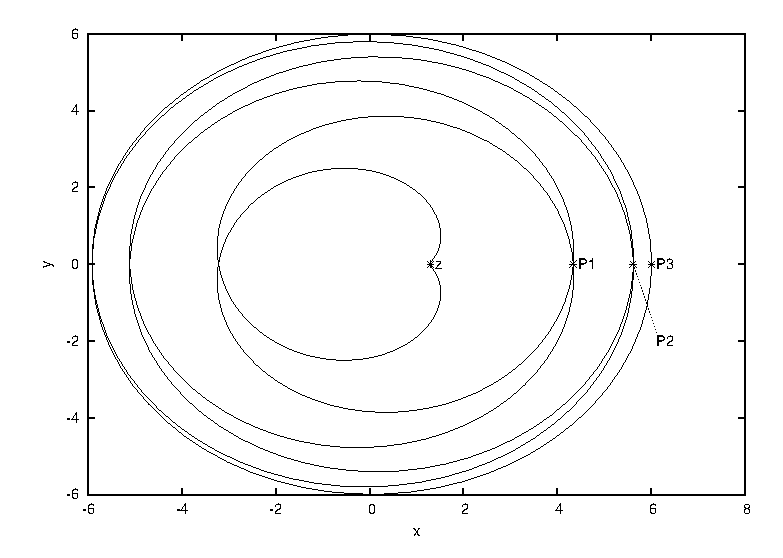
\includegraphics{figs/trtbp}
\caption{Resonant periodic orbit $\gamma_{-1.6}$ of the circular
problem in rotating cartesian coordinates.}
\label{fig:trtbp}
\end{figure}

For illustration, let us show some numerical results corresponding to
the energy value $H=-1.6$.
The first approximation $\tilde \gamma_{-1.6}$ from the two-body
problem has initial condition $p^0=(x^0,p_x^0)=(1.30253\cdots,0)$.
After refining this initial condition via the Newton method, we obtain
a resonant periodic orbit $\gamma_{-1.6}$ of the circular problem passing
through the point $p=(x,p_x)=(1.29858\cdots,0)$, with period
$T_{-1.6}=44.01796\cdots \sim 14\pi$. See Figure~\ref{fig:trtbp}. 
The periodic orbit $\gamma_{-1.6}$ is symmetric, with the points $p$
and $P^3(p)$ located at the symmetry section (they have $y=0$ and $p_x=0$).
Notice that, in rotating coordinates, the trajectory of the Asteroid
makes 6 turns around the origin before closing up at the point $p$.

\begin{figure}
\psfrag{H}{$H$}
\psfrag{T}{$T_H - 14\pi$}
\psfrag{T2XXXXXXX}{$T_H - 14\pi$}
\psfrag{L2XXXXXXX}{$L_{\max}$}
\includegraphics{figs/porbits}
\caption{Resonant family of periodic orbits.
We show normalized period $T_H - 14\pi$, and maximum deviation of $L$
component with respect to the resonant value $7^{1/3}$ (see
equation~\eqref{eq:Ldeviation}).}
\label{fig:porbits}
\end{figure}

Finally, we let $H$ change and, using this procedure, we are able to
obtain the resonant periodic orbit for energy levels 
\[ H \in [\bar H_-, \bar H_+] = [-2.04,-1.56]. \] 
See Figure~\ref{fig:porbits}.
This family of resonant periodic orbits constitutes the normally
hyperbolic invariant manifold $\Lambda_0$ given in
Corollary~\ref{coro:NHIMCircular}. 
Notice that the period $T_H$ stays close to the resonant period $14\pi$ of the unperturbed system.
From Figure~\ref{fig:porbits}, we obtain the bound
\[ |T_H - 14\pi| < 60\mu, \]
which is the first bound given in Theorem \ref{th:NHIMCircular}.


To determine the stability of the periodic orbit $\gamma_h$, we
compute the eigenvalues $\lambda$ and $\lambda^{-1}$ of the matrix
$DP^6(p)$, where $DP^6(p)$ is the linearization of the iterated
Poincar\'e map $P^6$ about the fixed point $p$. 
(Since $DP^6(p)$ is a $2\times2$ matrix, the eigenvalues are trivial
to compute.)

\begin{figure}
\psfrag{H}{$J$}
\psfrag{lu}{$\ln(\lambda)$}
\includegraphics{figs/hypers}
\caption{Characteristic exponent $\ln(\lambda)$ as a function of
energy level $J$ (the other exponent is $-\ln(\lambda)$).}
\label{fig:hypers}
\end{figure}

Figure~\ref{fig:hypers} shows the characteristic exponents
$\ln(\lambda)$, $\ln(\lambda^{-1})$ as a function of energy.
The family of periodic orbits is strongly hyperbolic as $H \to \bar
H_+$, and weakly hyperbolic as $H\to \bar H_-$.
Note that one would expect that we are in a  nearly integrable regime
since $\mu$ is small. Then one would expect the eigenvalues to be
close to 1.
Nevertheless, in this problem the non-integrability is very noticeable
when one increases $\mu$ to $\mu=\mu_J=10^{-3}$. This is due to the effect of
the perturbing body (Jupiter) on the Asteroid, as the Asteroid passes
close to it.

Furthermore, we verify that the (square of the) semi-major axis $L$ stays
close to the resonant value $7^{1/3}$.
Integrating the periodic orbit in Delaunay coordinates
$\gamma_H(t)=(L(t),\ell(t),G(t),g(t))$ over one period $T_H$, we compute
the quantity
\begin{equation} \label{eq:Ldeviation}
 L_{\max}(H) = \max_{t \in [0,T_H)} |L_H(t)-7^{1/3}|.
\end{equation}
The function $L_{\max}(H)$ is plotted in figure~\ref{fig:porbits}.
Notice that we obtain the bound
\[ |L_H(t)-7^{1/3}| < 7\mu \]
for all $t\in \RR$, which is stated in Theorem \ref{th:NHIMCircular}.

\begin{figure}
\psfrag{x}{$x$}
\psfrag{y}{$y$}
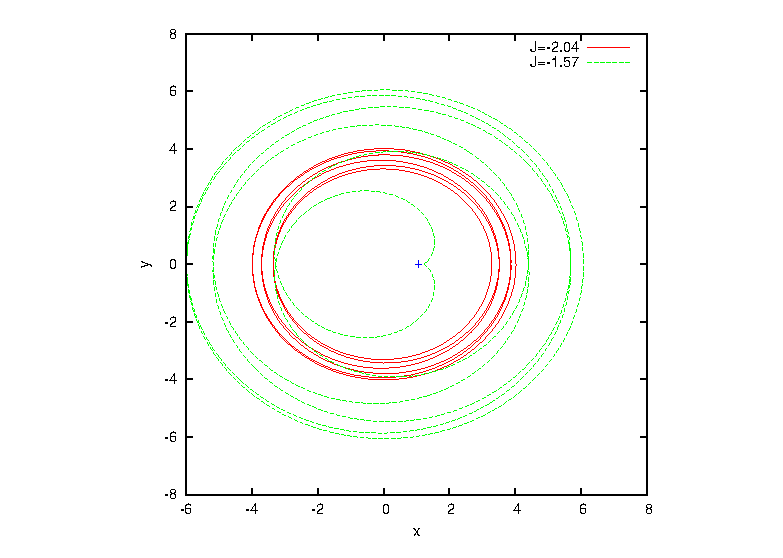
\includegraphics{figs/trtbp_porbits}
\caption{Extremal periodic orbits of the family: circular periodic
orbit with $H=\bar H_-$ (in red), elliptical periodic orbit with
$H=\bar H_+$ (in green). The Lagrange equilibrium point $L_2$ is
marked with a '+' symbol.}
\label{fig:trtbp_porbits}
\end{figure}

Let us briefly describe the family of periodic orbits $\gamma_H$. 
For illustration, see Figure~\ref{fig:trtbp_porbits}.

XXXXX PR: We should try to explain the family in terms of bifurcations
of periodic orbits. XXXXX

At one endpoint of the family, as $H \to \bar H_-$, the periodic orbit
$\gamma_H$ tends to a circular orbit of period $14\pi$ centered at the
origin and passing far away from the primaries (Sun and Jupiter).
Moreover, $\gamma_H$ looses hyperbolicity when $H \to \bar H_-$.
For instance, the periodic orbit $\tilde \gamma(\bar H_-)$ of the two-body
problem approximation has eccentricity $e(\bar H_-)=0.09989\cdots$.

At the other endpoint of the family, as $H \to \bar H_+$, the periodic
orbit $\gamma_H$ tends to a homoclinic loop of the Lagrangian
equilibrium point $L_2$ that makes $6$ turns around the Sun-Jupiter
system. 
(In rotating cartesian coordinates, $L_2$ is located on the $x$ axis at
the point $x_2 \simeq 1.068$).\ 
This explains the fact that the period $T_H$ ``explodes'' as $H \to
\bar H_+$. Since we are interested in working close to the resonance,
we avoid energies $H > \bar H_+$ where the period explodes.


\subsection{Computation of invariant manifolds}
\label{sec:invariant_manifolds}


In this section, we compute the stable and unstable invariant
manifolds associated to the periodic orbits found in the previous
section. 

Consider first a fixed energy level $H=h$.
Let $\gamma_h$ be the resonant periodic orbit of the circular problem
found in the previous section. 
To compute the invariant manifolds of the periodic orbit, we continue
using the iterated Poincar{\'e} map.
Thus we look for (one dimensional) invariant manifolds of a hyperbolic
fixed point at each energy level.  
Let $p \in \gamma_h$ be a hyperbolic fixed point of the iterated
Poincar\'e map $\sixmap = P^6$. 
Let $\lambda, \ \lambda^{-1}$ be the eigenvalues of $D\sixmap(z)$ with
$\lambda>1$, and $v_u, v_s$ be the associated eigenvectors.

Assume that we want to compute the unstable manifold $W^u(p)$.
Let $\eta$ be a small displacement in the unstable direction $v_u$.
We approximate a piece of the local manifold by the linear segment
between the points $p+\eta v_u$ and $\sixmap(p+\eta v_u)$.
We call this segment a \emph{fundamental domain}.
We discretize the fundamental domain into an array of points, and
iterate them by $\sixmap$ to globalize the manifold.
(The stable manifold is computed analogously using the inverse map
$\sixmap^{-1}$.)

The error commited in the local approximation
$ \sixmap(p+\eta v_u) = p + \lambda \eta v_u + \OO(\eta^2) $
of the manifold is given by
\[ \mathrm{err}(\eta) = \left\|\sixmap(p+\eta v_u) - p - \lambda \eta v_u \right\| \in \OO(\eta^2).
\]
%Similarly, in the stable case,
%\[ err_s(\eta) =  ||\sixmap^{-1}(z+\eta v_s)-z-\frac{1}{\rho_s}\eta v_s|| \in
%O(\eta^2). \]

\begin{remark} \label{rem:displacement}
For each energy level $H$, we choose a displacement $\eta=\eta(H)$
such that the local error is $\mathrm{err}(\eta) < 10^{-12}$.
\end{remark}

\begin{figure}
\psfrag{x}{$x$}
\psfrag{px}{$p_x$}
\psfrag{p0}{$p_0$}
\psfrag{p1}{$p_1$}
\psfrag{p2}{$p_2$}
\psfrag{p3}{$p_3$}
\psfrag{p4}{$p_4$}
\psfrag{p5}{$p_5$}
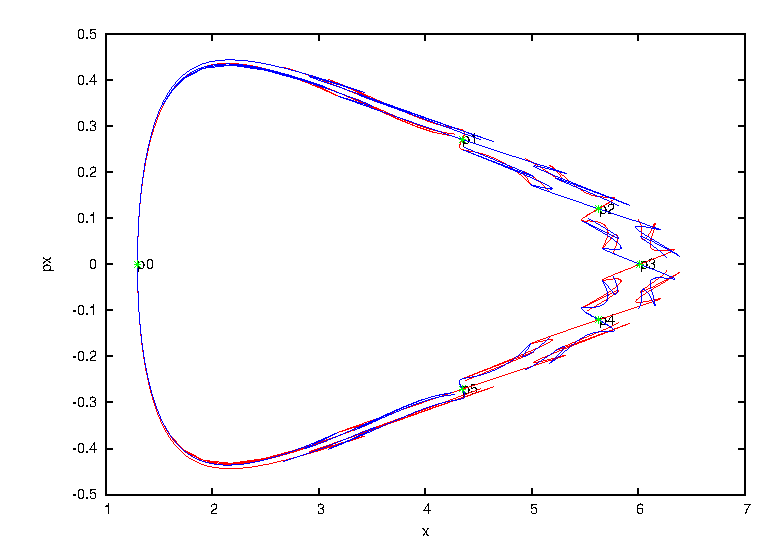
\includegraphics{figs/invmfld_it}
\caption{Invariant manifolds of the fixed points $p_0, p_1,\dots,p_5$
on the section $\Sigma^+$.
Unstable manifolds are plotted in red, stable in blue.
The fixed points are marked in green.}
\label{fig:invmfld_it}
\end{figure}

One can think of $p$ as a fixed point of the iterated Poincar\'e map
$\sixmap = P^6$, or as a $6$-periodic point of the Poincar\'e map $P$.
If $p_i = P^i(p)$ are the iterates of $p$ for $i=0,\dots,5$, then
$p_i$ are also fixed points of $\sixmap$. 
They have associated unstable and stable manifolds, which can be obtained from
$W^{u,s}(p)$ by iteration.

For illustration, let us show some numerical results corresponding to
the energy value $H=-1.6$.
Figure~\ref{fig:invmfld_it} shows the manifolds of all iterates
$\{p_i\}_{i=0,\dots,5}$.
Notice that the dynamics in Figure~\ref{fig:invmfld_it} is reversible
with respect to the symmetry section $\{y=0,\ p_x=0\}$, as discussed
in the previous section (equation~\eqref{involutionCartesian}).
Figure~\ref{fig:invmfld_it} shows that the manifolds do intersect
transversally at different homoclinic points.
We are interested in measuring the splitting angle between the
manifolds.
Unfortunately, the homoclinic points do not lie on the symmetry axis, which
would be very useful in order to compute them.

\begin{figure}
\psfrag{x}{$x$}
\psfrag{px}{$p_x$}
\psfrag{p0}{$p_0$}
\psfrag{p1}{$p_1$}
\psfrag{p2}{$p_2$}
\psfrag{p3}{$p_3$}
\psfrag{p4}{$p_4$}
\psfrag{p5}{$p_5$}
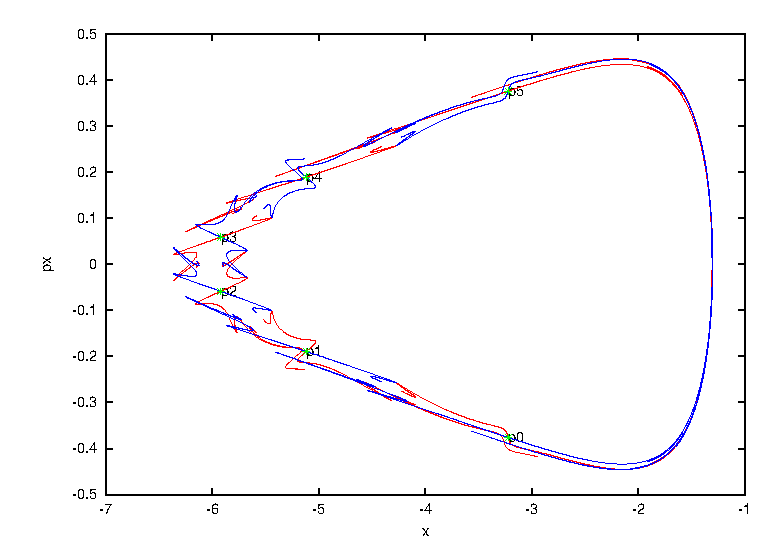
\includegraphics{figs/invmfld2}
\caption{Invariant manifolds on the section $\Sigma^-$.}
\label{fig:invmfld2}
\end{figure}

\begin{figure}
\psfrag{x}{$x$}
\psfrag{px}{$p_x$}
\psfrag{p2}{$p_2$}
\psfrag{p3}{$p_3$}
\psfrag{Wu1p3}{$W^{u,1}(p_3)$}
\psfrag{Ws2p3}{$W^{s,2}(p_3)$}
\psfrag{Ws1p2}{$W^{s,1}(p_2)$}
\psfrag{Wu2p2}{$W^{u,2}(p_2)$}
\includegraphics{figs/invmfld2_it23}
\caption{Invariant manifolds of the points $p_2$ and $p_3$ on the
section $\Sigma^-$. Due to the symmetry, points that lie on the line
$p_x=0$ (marked in green) are intersection points.}
\label{fig:invmfld2_it23}
\end{figure}


In order to have the homoclinic points lie on the symmetry axis, we
recompute the manifolds on the new Poincar\'e section
\[ \Sigma^- = \{y=0,\ p_y<0\}. \]
Numerically, we just transport points on the unstable manifold from
section $\Sigma^+$ to section $\Sigma^-$ by the forward flow, and
points in the stable manifold by the backward flow.
See Figures~\ref{fig:invmfld2} and~\ref{fig:invmfld2_it23}.
Now the points that lie on the symmetry line $p_x=0$ are homoclinic
points.


\subsection{Computation of transversal homoclinic points and splitting
angle}
\label{sec:homoclinic_points}


In this section, we compute the angle between the invariant manifolds
at one of the  transversal intersections. 
We will restrict the range of energy values to
\[ H\in[H_-,H_+]=[-1.81,-1.56], \]
or equivalently the range of eccentricities to
$ e\in[e_-,e_+]=[0.48,0.66]$.
This is the range where we can validate the accuracy of our
computations (see section~\ref{sec:accuracy_computations}).
Below $e_-=0.48$, the splitting size becomes comparable to the
numerical error that we commit in double precision arithmetic. 

\begin{remark}
In this paper we concentrate on proving the existence of global
instabilities in the Restricted three-body problem; we are not so much
concerned with finding the \emph{maximal} range of eccentricities
along which the Asteroid drifts.
Thus we do not investigate the behavior of the splitting below
$e_-$.
However, we are convinced that the maximal range of eccentricities is
larger than $[e_-,e_+]$, in particular that the lower bound can be
pushed well below $e_-$.  
We think that our mechanism of instability applies to this larger
range of eccentricities.
In fact, it is possible to study such exponentially small splitting
using more sophisticated numerical methods, such as multiple-precision
arithmetic, and high-order approximation of local invariant manifolds,
see for instance~\cite{FontichSimo1990, DelshamsRamirez1999,
GelfreichSimo2008}.
\end{remark}

\begin{figure}
\psfrag{x}{$x$}
\psfrag{px}{$p_x$}
\psfrag{p2}{$p_2$}
\psfrag{p3}{$p_3$}
\psfrag{z1}{$z_1$}
\psfrag{z2}{$z_2$}
\psfrag{Wu1p3}{$W^{u,1}(p_3)$}
\psfrag{Ws2p3}{$W^{s,2}(p_3)$}
\psfrag{Ws1p2}{$W^{s,1}(p_2)$}
\psfrag{Wu2p2}{$W^{u,2}(p_2)$}
\includegraphics{figs/invmfld2_it23_H174}
\caption{Invariant manifolds of the points $p_2$ and $p_3$ for the energy
level $H=-1.74$.}
\label{fig:invmfld2_it23_H174}
\end{figure}

Consider first a fixed energy level $H=h$ that is close to the
unperturbed situation, e.g. $H=-1.74$. 
The corresponding manifolds are given in
Figure~\ref{fig:invmfld2_it23_H174}.
In general, there are uncountably many intersection points.
For instance, in Figure~\ref{fig:invmfld2_it23} we show six intersections on
the symmetry line.
However, when the perturbation is small, there is one distinguished
intersection point located ``in the middle'' of the homoclinic.
We call it the \emph{primary} intersection point.

Let us compute the primary intersection point $z_1$ corresponding to
the ``outer'' splitting of the manifolds $W^{u,1}(p_3)$ and
$W^{s,1}(p_2)$.
For $H=-1.74$, the \emph{primary} intersection $z_1$ corresponds to
the \emph{first} intersection of the manifolds with the $p_x=0$ line,
as we grow the manifolds from the fix points.
Thanks to the symmetry, it is enough to look for the intersection of
$W^{u,1}(p_3)$ with the $p_x=0$ axis, because $W^{s,1}(p_2)$ must also
intersect the axis at the same point.

To compute the intersection point $z_1$, we continue using a linear
approximation of the local manifold, and propagate a fundamental
domain in the local manifold by iteration.
Let $v_u$ be the unstable eigenvector associated to the point $p_3$.
Consider the fundamental segment $l_u$ between the points $p_3+\eta
v_u$ and $\sixmap(p_3+\eta v_u)$, as in the previous section.
First we look for the \emph{smallest} natural $n$ such that
$\sixmap^n(l_u)$ intersects the $p_x=0$ axis.
%(For our example periodic orbit $\gamma_{-1.74}$ we need $n=15$
%iterations.)
Then we use a standard numerical method (bisection-like
one-dimensional root finding) to find a point $z_u$ in the fundamental
segment $l_u$ such that
\[ \pi_{p_x}(\sixmap^{n}(z_u))=0. \]
Thus we obtain the homoclinic point $z_1 = \sixmap^{n}(z_u)$ in
Figure~\ref{fig:invmfld2_it23_H174}.
Numerically, we verify that $z_1$ is in the the $p_x=0$ axis within
$10^{-10}$ tolerance.

\begin{figure}
\psfrag{H}{$H$}
\psfrag{x}{$x$}
\includegraphics{figs/intersec}
\caption{Family of primary intersection points corresponding to outer
and inner splitting. 
For every energy level $H$, we plot the $x$ coordinate of the
intersection point $z_1$ and $z_2$ (the $p_x$ coordinate is equal to
zero). Notice that both families are continuous.}
\label{fig:intersec}
\end{figure}

Finally, we vary energy $H$ and use a continuation method to obtain
the family of primary intersections $\{z_1\}_H$, using as seed the
primary intersection $z_1(H=-1.74)$ found above.
See Figure~\ref{fig:intersec}.

\begin{remark}
For low energy levels (such as $H=-1.74$), corresponding to weak
hyperbolicity, the invariant manifolds behave as if they were close to
integrable, and the primary intersection corresponds to the
\emph{first} intersection of the manifolds with the $p_x=0$ axis.
For high energy levels (such as $H=-1.6$), corresponding to strong
hyperbolicity, the manifolds develop some folds, and thus the primary
intersection may not correspond to the \emph{first} intersection of
the manifolds with the $p_x=0$ axis. See
Figure~\ref{fig:invmfld2_it23}.

In practice, we first identify the primary intersection at low energy
levels, and then use a continuation method to obtain. the primary
family of intersections up to high energy levels.
\end{remark}

Analogously, we compute the family of primary intersections
$\{z_2\}_H$ corresponding to the inner splitting.
See Figure~\ref{fig:intersec}.

Let us now compute the splitting angle between the manifolds $W^{u,1}(p_3)$
and $W^{s,1}(p_2)$ at the point $z_1$.
For illustration, we show some numerical results corresponding
to the energy value $H=-1.74$.
First we need the tangent vectors $w_u$ and $w_s$ to the manifolds at
$z_1$. See Figure~\ref{fig:splitangle}.
As found above, let $z_u$ be the point in the unstable fundamental
segment that maps to $z_1$, i.e. $\sixmap^{n}(z_u) = z_1$.
Consider the tangent vector $v_u$ to the manifold $W^{u,1}(p_3)$ at
the point $z_u$. 
(Recall that at this point the linear approximation is good enough, so
we can use as $v_u$ the unstable eigenvector.)
Multiply $v_u$ by the Jacobian of $\sixmap$ at the successive iterates
$\sixmap^{i}(p_u)$, for $i=0,...,n-1$.
This way, we obtain the tangent vector to the unstable manifold at
$z_1$. Let us denote this vector $w_u=(w_1,w_2)$.
We normalize it to $||w_u||=1$.

\begin{figure}
\psfrag{x}{$x$}
\psfrag{px}{$p_x$}
\psfrag{z}{$z_1$}
\psfrag{wu}{$w_u$}
\psfrag{ws}{$w_s$}
\includegraphics{figs/splitangle}
\caption{Outer splitting of the manifolds for energy level $H=-1.74$. 
This is a magnification of Figure~\ref{fig:invmfld2_it23_H174} at the
intersection point~$z_1$. 
We show the vectors $w_u, w_s$ tangent to the unstable and stable
manifolds at $z_1$. 
The splitting angle $\sigma$ is the angle between $w_u$ and $w_s$.}
\label{fig:splitangle}
\end{figure}

Due to reversibility, the vector $w_s$ tangent to the stable manifold
at $z_1$
is $w_s=(w_1,-w_2)$. See Figure~\ref{fig:splitangle}. Notice that we
choose the tangent vectors with the appropriate orientation, i.e. with
the same orientation as the trajectories on the manifolds. 

Thus the oriented splitting angle between $w_u$ and $w_s$ is 
\[ \sigma= 2\arctan_2(-w_1,-w_2), \]
where $\arctan_2$ is the arctangent function of two variables, which
uses the signs of the two arguments to determine the sign of the
result.

\begin{figure}
\psfrag{H}{$H$}
\psfrag{s}{$\sigma$ (radians)}
\includegraphics{figs/splittings}
\caption{Splitting angle associated to inner and outer splitting.}
\label{fig:splittings}
\end{figure}

\begin{table}
\begin{tabular}{|c|c|}
\hline
inner & outer \\
\hline
$ ( -1.695,-1.694 ) $ & $ ( -1.701,-1.700 ) $ \\
$ ( -1.726,-1.725 ) $ & $( -1.731,-1.730 ) $ \\
$ ( -1.756,-1.755 ) $ & $ ( -1.760,-1.759 ) $ \\
$ ( -1.781,-1.780 ) $ & $ ( -1.784,-1.783 ) $ \\
$ ( -1.802,-1.801 ) $ & $ ( -1.805,-1.804 ) $ \\
\hline
\end{tabular}
\caption{Subintervals of $H\in[H_-,H_+]$ containing the zeros of inner
splitting (left column) and outer splitting (right column).}
\label{tab:zeros_inner_outer}
\end{table}



Finally, we let $H$ change and, using this procedure, we are able to
obtain the splitting angle for energy levels $H \in [H_-, H_+]$.
See Figure~\ref{fig:splittings}.
The splitting angle is nonzero for all energy values except for a
discrete set of them.  
The splitting angle oscillates around zero with decreasing amplitude
as $H\to H_-$.
Numerically, we find that the zeros of the splitting angle are
contained in the intervals listed in
Table~\ref{tab:zeros_inner_outer}.

Notice that the inner and outer splittings behave similarly.
%See Figure~\ref{fig:splittings}.
However, they become zero at different values of $H$, as seen in
Table~\ref{tab:zeros_inner_outer}.
Thus, when one of the intersections becomes tangent, the other one is
still transversal, and we can always use one of them for diffusion. 


\subsection{Accuracy of the Computations}
\label{sec:accuracy_computations}

For small eccentricities, the splitting angle~$\sigma$ becomes very
small.
We need to check the validity of $\sigma$, making sure that the size
of (accumulated) numerical errors in the computation is smaller than
the size of $\sigma$.

The smallest splitting angle in Figure~\ref{fig:splittings},
corresponding to $H_-=-1.81$, is
\[ \sigma(H_-)= -1.777970294158603 \times 10^{-5}. \]
We check the validity of $\sigma(H_-)$ by recomputing this angle using
an alternative numerical method.
First we compute the intersection of the manifolds $W^{u,1}(p_3)$ and
$W^{s,1}(p_2)$ with the horizontal axis defined by
\[ p_x = \frac{j}{10^{5}} \]
for $j\in (-2,-1,1,2)$.

\begin{table}
\begin{tabular}{|c|c|c|c|}
\hline
$p_x$ & $x^u$ & $x^s$ & $x^u-x^s$ \\
\hline
$-0.00002$ & $-5.481541931871417$ & $-5.481541932226887$ &
$0.000000000355470$ \\
$-0.00001$ & $-5.481541931790012$ & $-5.481541931967703$ &
$0.000000000177691$ \\
$0.00000$ & $-5.481541931822124$ & $-5.481541931822124$ &
$0.000000000000000$ \\
$0.00001$ & $-5.481541931967703$ & $-5.481541931790012$ &
$-0.000000000177691$ \\
$0.00002$ & $-5.481541932226887$ & $-5.481541931871417$ &
$-0.000000000355470$\\
\hline
\end{tabular}
\caption{Sampling of the manifolds $W^{u,1}(p_3)$ and $W^{s,1}(p_2)$ at
different values of $p_x$, and their difference (last column).}
\label{tab:differentiation}
\end{table}

In Table~\ref{tab:differentiation} we tabulate the $x$ coordinate of
$W^{u,1}(p_3)$ and $W^{s,1}(p_2)$ on these axis, and their difference
$d=x^u-x^s$ gives the distance between the manifolds.
We apply numerical differentiation to the last column of this table,
using central differences centered at $z_1$ with step sizes $0.00002$
and $0.00004$, and obtain the values:
\[ d_1 = \frac{d(0.00001) - d(-0.00001)}{0.00002} =
-0.0000177691.\]
\[ d_2 = \frac{d(0.00002) - d(-0.00002)}{0.00004} =
-0.0000177735.\]
Finally, we use Richardson extrapolation and obtain:
\[ d = \frac{4 d_1-d_2}{3} = -0.00001776763333333333. \]
Thus, using this alternative method, we obtain the splitting angle
\[ \sigma(H_-) = \mathrm{atan}(-0.00001776763333333333) =
-0.00001776763333146364. \]
Compare the splitting angle computed using the two methods. They
differ by approximately $10^{-8}$.
This gives an estimate of the numerical error commited in our
computation of the splitting angle.

\begin{figure}
\psfrag{H}{$H$}
\psfrag{srad}{$\sigma$ (radians)}
\psfrag{s}{$\sigma$}
\psfrag{err}{$\mathrm{err}$}
\includegraphics{figs/diffs}
\caption{Splitting angle $\sigma(H)$ and estimate of the numerical
error $\mathrm{err}(H)$ as a function of energy level $H$.}
\label{fig:diffs}
\end{figure}

We repeat this test for a range of energies $H\in[-1.81,-1.8]$.
In Figure~\ref{fig:diffs}, we compare the splitting angle $\sigma(H)$
and the estimate of the numerical error $\mathrm{err}(H)$. This error stays
below $10^{-7}$, and it is several orders of magnitude smaller than
the splitting angle.
For higher energy values $H\in[-1.8,-1.56]$, the splitting angle is
large, so the numerical error is certainly smaller.
Therefore we are confident that the splitting angle has been accurately
computed in the range of eccentricities considered,
$[H_-,H_+]$.


\section{Geometric structure of the resonance in Delaunay coordinates}
\label{sec:geometric_structure_delaunay}

Explain that the Poincar\'e sections in Cartesian and Delaunay are very
different. Explain that, after we transform periodic points to
Delaunay, we have to flow them a little forward or backwards until
they lie on the {g=0} section.

Show a picture of the resonance (periodic points, inv. manifolds) in
Delaunay.

\section{Numerical study of the inner and outer dynamics}
\label{sec:NumericalStudyInnerOuter}

\subsection{Inner and outer dynamics of the circular problem}
\label{app:InnerOuterCircular}

In this section, we numerically compute the inner map $\FF_0^\inn$ and
the outer maps $\FF_0^{\out,\ast}$ of the circular problem, given in
Section~\ref{Section:Circular}.
XXX Change of notation: $H$ instead of $I$. XXX

As seen in Section~\ref{sec:Circular:Inner}, the inner map has the
form
\begin{equation}\label{def:InnerMap:Circular:Numerics}
  \FF_0^\inn:\left(\begin{array}{c} H\\
      t
    \end{array}\right)\mapsto \left(\begin{array}{c} H\\
      t+\mu\TTT_0(H)
    \end{array}\right),
\end{equation}
where $T_H = 14\pi + \mu\TTT_0(H)$ is the period of the periodic orbit
obtained in Theorem~\ref{th:NHIMCircular} on the corresponding energy
surface.

Recall that we computed the periodic orbit $\gamma_H$ as well as its
period $T_H$ in Section~\ref{sec:computation_periodic_orbits}.
In particular, Figure~\ref{fig:porbits} shows a plot of the function
$T_H - 14\pi = \mu\TTT_0(H)$. 
Notice that the derivative of the function $\TTT_0(H)$ is nonzero for
the whole range $[\bar H_-, \bar H_+]$ of energy values. 
This shows that the inner map is twist. 
Moreover, Figure~\ref{fig:porbits} shows that 
\[ 0<\mu\TTT_0(H)<60\mu<\pi. \]
Therefore, the function $\TTT_0(H)$ satisfies the properties
stated in Lemma~\ref{lem:TwistInner}

As a test, we have computed the same function $\TTT_0(H)$ using two
different methods. First by computing the period of the periodic
orbit, as above. Then by computing the integral
expression~\eqref{def:T0:Integral} using numerical integration. The
difference in $\TTT_0(H)$ using both methods is of the order
$10^{-12}$.

As seen in Section~\ref{sec:Circular:Outer}, the outer maps have the
form
\begin{equation}\label{def:OuterMap:Circular:Numerics}
  \FF_0^{\out,\ast}:\left(\begin{array}{c} H\\
      t
    \end{array}\right)\mapsto \left(\begin{array}{c} H\\
      t+\mu\omega^\ast(H)
    \end{array}\right),\,\,\,\ast=\ff,\bb.
\end{equation}
For simplicity, let us only discuss the computation of $\omega^\ff(H)$
($\omega^\bb(H)$ is computed analogously).
Recall from Lemma~\ref{lem:Omega0} that the function $\omega^\ff(H)$
is defined as
  \[
  \omega^\ff(H)= \omega^\ff_\out(H)+\omega_\inn^\ff (H),
  \]
where, taking into account that the homoclinic orbit is symmetric with respect to the involution \eqref{def:involution},
\begin{equation}\label{def:Omega0:OuterPart:Numerics}
 \omega^\ff_\out(H)=\omega_+^\ff(H)-\omega^\ff_-(H) = 2\omega_+^\ff(H)
\end{equation}
  with
  \begin{equation}\label{def:Omega0PlusMinus:Numerics}
 \begin{split}  
 \omega_+^\ff(H)&=\lim_{N\rightarrow+\infty}\left(\int_0^{ 14N\pi
      }\frac{(\pa_G\Delta
        H_\ccirc) \circ \gamma_H^\ff(\sigma)}{-1+\mu(\pa_G\Delta
        H_\ccirc) \circ \gamma_H^\ff(\sigma)} \,
d\sigma+N\TTT_0(H)\right),\,\,\,
\end{split}  
\end{equation}
\begin{equation}\label{def:Omega0:InnerPart:Numerics}
\begin{split}
 \omega_\inn^\ff(H)&=\int_0^{ -12\pi
      }\frac{(\pa_G\Delta
        H_\ccirc) \circ \gamma_H^4(\sigma)}{-1+\mu(\pa_G\Delta
        H_\ccirc) \circ \gamma_H^4(\sigma)} \, d\sigma.
\end{split}
\end{equation}
To obtain $\omega^\ff(H)$, we compute the
integrals~\eqref{def:Omega0PlusMinus:Numerics}
and~\eqref{def:Omega0:InnerPart:Numerics} numerically, using a standard
algorithm from the GSL library XXX Add reference XXX.
The integrals are computed within a relative error limit $10^{-9}$.

The function $\pa_G\Delta H_\ccirc$ involved in both integrals is
given explicitly in Appendix~\ref{sec:RotatingToDelaunay}.
The integral $\omega_\inn^\ff(H)$ is evaluated on a periodic
trajectory $\gamma_H^4(\sigma)$ of the circular problem with initial
condition $p_4$, a fixed point of the Poincar\'e map $\PP_0^7$
found in Section~\ref{sec:geometric_structure_delaunay}.
The integral $\omega_+^\ff(H)$ is evaluated on a homoclinic trajectory
$\gamma_H^\ff(\sigma)$ of the circular problem with initial condition
$z_2$, the primary homoclinic point corresponding to the inner
splitting found in Section~\ref{sec:homoclinic_points}.

Next we make a couple of important remarks about the numerical
computation of the integral $\omega_+^\ff(H)$.
The key point is that the homoclinic orbit $\gamma_H^\ff$ was already
computed in section~\ref{sec:homoclinic_points} with high accuracy,
and we can exploit this information here.
Recall that the primary homoclinic point $z_2$ was obtained as the
$n$-th iterate of a point $z_u$ in the local fundamental segment $l_u$
under the Poincar\'e map:
\begin{equation} \label{eq:zu_to_z2}
 z_2 = \{\PP_0^7\}^n (z_u).
\end{equation}
Moreover, recall that the point $z_u$ was chosen to be suitably close
to the fixed point $p_3$ for each energy level $H$.
See Remark~\ref{rem:displacement}. 

Notice that the integral $\omega_+^\ff(H)$ is defined by a limit as
$N\to\infty$, i.e. as the homoclinic orbit $\gamma_H^\ff(\sigma)$
assymptotically approaches the periodic orbit $\gamma_H^3(\sigma)$ in
forward time (see equation~\eqref{def:OmegaSmall}).
Numerically, of course, we should stop integrating at an upper
endpoint $N$ large enough such that the integral converges. 
In practice, we choose the upper endpoint $N=N(H)$ to be the number of
iterates $n=n(H)$ in~\eqref{eq:zu_to_z2}.
This means that we evaluate the integral along the homoclinic
trajectory $\gamma_H^\ff(\sigma)$ until it reaches the point $z_u$,
which is suitably close to the periodic orbit.

Notice also that integrating the homoclinic trajectory
$\gamma_H^\ff(\sigma)$ forwards in the reduced system means
integrating it backwards along the unstable manifold in the original
system. 
This is numerically unstable, since numerical errors grow
exponentially. 
In practice, we rewrite the
integral~\eqref{def:Omega0PlusMinus:Numerics} using the change of
variables $\hat \sigma = \sigma - 14N\pi$ so that the homoclinic
trajectory is integrated forwards along the unstable manifold,
starting from the point $z_u$.

\begin{figure}
\psfrag{H}{$H$}
\psfrag{wf}{$\omega^{\ff}$}
\psfrag{wb}{$\omega^{\bb}$}
\includegraphics{figs/omega_fb}
\caption{Functions $\omega^{\ff}$ and $\omega^{\bb}$ involved in the
definition of the outer map~\eqref{def:OuterMap:Circular:Numerics} of
the circular problem.}
\label{fig:outer_circular}
\end{figure}

The computed values of the functions $\omega^{\ff}$ and $\omega^{\bb}$
are shown in Figure~\ref{fig:outer_circular}.

To test the computation of the function $\omega_+^\ff$, we directly
verify the definition of the outer map~\ref{definition:OuterMap}.
Let $z_2 = (L_h,\ell_h,G_h,0)$ be the primary homoclinic point, and
let $p_3 = (L_p,\ell_p,G_p,0)$ be the periodic point. 
Given a point $(L_h,\ell_h,G_h,0, I, t)$ in the extended circular
problem, we check that it is forward assymptotic (in the
reparametrized time) to the point $(L_p,\ell_p,G_p,0, I,
t+\omega_+^\ff)$, where $t\in\TT$ is arbitrary.
Thus we check that the distance
\[ \mathrm{dist}^+(s) = |\Phi_0\{s,(L_h,\ell_h,G_h,0, I, t)\} - 
\Phi_0\{s,(L_p,\ell_p,G_p,0, I, t+\omega_+^\ff)\}| 
\xrightarrow{s\to\infty} 0 \]
with exponential decay.

\begin{figure}
\psfrag{N}{$N$}
\psfrag{d}{$dist^+$}
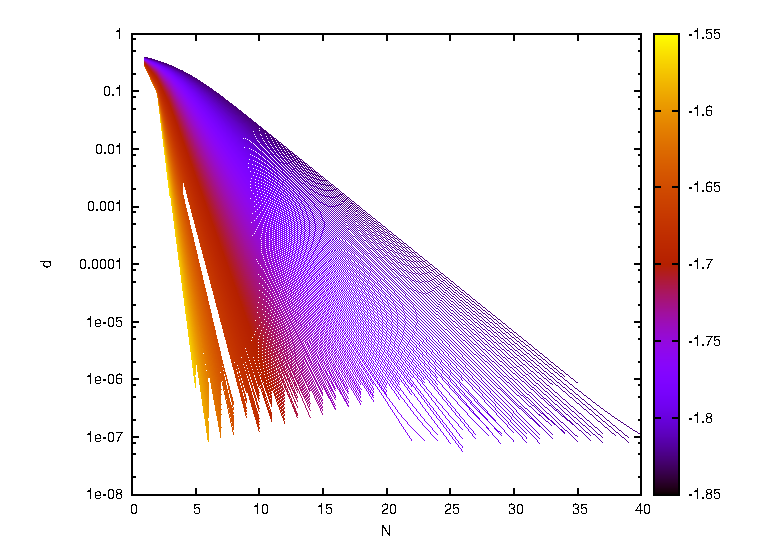
\includegraphics{figs/outer_circ_test}
\caption{Exponential decay of the function $\mathrm{dist}^+$ as a function of
$N$ (multiples of the period) for different energy levels.
The energy levels $H\in[H_-,H_+]$ are color-coded.}
\label{fig:outer_circ_test}
\end{figure}

The result of the test is shown in Figure~\ref{fig:outer_circ_test}
for values of the energy $H\in[H_-,H_+]$.  
Notice that the vertical axis is in logarithmic scale. 
Let $s=14N\pi$. 
We plot the distance $\mathrm{dist}^+$ as a function of $N$ (multiples of the
period). 
The test shows exponential decay of the distance function for all
energy values, i.e. straight lines in the plot. 

Recall that the periodic orbit $\gamma_H$ becomes more hyperbolic as
the energy $H$ increases. Thus, the rate of exponential convergence
between the homoclinic and the periodic trajectory also increases,
i.e. the straight lines have increasing slope in the plot.
As explained above, the length of integration $N=N(H)$ along the
homoclinic orbit is suitably chosen for each energy level.
For energy values $H\to H_-$, there is exponential decay up to
time $s=40\cdot (14\pi) \approx 1760$.



\subsection{Inner and outer dynamics of the elliptic problem}
\label{app:InnerOuterElliptic}

In this section, we numerically compute the first orders in $e_0$ of
the inner map $\FF_{e_0}^\inn$ and the outer maps
$\FF_{e_0}^{\out,\ast}$ of the elliptic problem, given in
Section~\ref{sec:Elliptic}. 
In order to compare the inner and outer dynamics of the elliptic
problem through Lemma~\ref{lemma:Averaging}, only some specific terms
in the expansions of the inner and outer maps are necessary. 
Namely, we only need to compute the term $A_1$ in the expansion of the
inner map~\eqref{def:InnerMap:ell}, and the term $B^*$ in the
expansion of the outer map~\eqref{def:OuterMap:Elliptic}.

Recall from section~\ref{sec:CylinderExpansion} that $A_1$ can be
split as 
  \[
  A_1(I,t)=A_1^+(I)e^{it}+A_1^-(I)e^{-it}.
  \]
Since $A_1^+$ and $A_1^-$ are complex conjugate, it is only necessary
to compute one of them. Let us compute the positive harmonic,
  \begin{equation}\label{def:A:plus:Numerics}
    A_1^+(I)=-i\mu\int_0^{-14\pi}\frac{\Delta H_{\eell}^{1,+}\circ
\gamma_I^3(\sigma)}{-1+\mu\pa_G\Delta
H_\ccirc\gamma_I^3(\sigma)}e^{i\wt\gamma_I^3(\sigma)}d\sigma.
  \end{equation}
Notice that the denominator is the same one used in the previous
section for the inner and outer dynamics of the circular problem. 
Next we give the numerator $i\Delta H_{\eell}^{1,+}$ explicitly.
Let 
  \begin{equation}\label{def:Ham:Elliptic:order1}
    \begin{split}
      \Delta H^1_\eell(L,\ell,G,g,t) =&
-\frac{1-\mu}{\mu}\BB_1\left(-\frac{r(L,\ell,G)}{\mu},v(L,\ell,G),g,t\right)\\
      &-\frac{\mu}{1-\mu}\BB_1\left(\frac{r(L,\ell,G)}{1-\mu},v(L,\ell,G),g,t\right),
    \end{split}
  \end{equation}
  where $\BB_1$ is the function defined in Lemma
\ref{lemma:ExpansionB}.
%%%%%%%%%%%%%%%%%%%%%%%%%%%%%
\begin{comment}
We write $B_1$ as a sum of harmonics 
\begin{align*}
B_1(r,v+g,t) 
   &= B_1^+(r,v+g)e^{it}+B_1^-(r,v+g)e^{-it} \\
   &=-\frac{1-r\cos(v+g)-i2r\sin(v+g)}{2\Delta^3(r,v+g)}e^{it}
-\frac{1-r\cos(v+g)+i2r\sin(v+g)}{2\Delta^3(r,v+g)}e^{-it}.
\end{align*}
Thus we have
\[ B_1^+(r,v+g) =
-\frac{1-r\cos(v+g)-i2r\sin(v+g)}{2\Delta^3(r,v+g)}. \]

Writing $\Delta H_{\eell}^1$ as a sum of harmonics, we have
\begin{equation}
  \begin{split}
\Delta H_{\eell}^{1,+} =&
-\frac{1-\mu}{\mu}\BB_1^+\left(-\frac{r(L,\ell,G)}{\mu},v(L,\ell,G),g,t\right)\\
      &-\frac{\mu}{1-\mu}\BB_1^+\left(\frac{r(L,\ell,G)}{1-\mu},v(L,\ell,G),g,t\right).
  \end{split}
\end{equation}
\end{comment}
%%%%%%%%%%%%%%%%%%%%%%%%%%%%%
Then it is straightforward to see that 
\begin{equation}
  \begin{split}
\Delta H_{\eell}^{1,+}(l,L,g,G)
=& 
-\frac{1-\mu}{\mu}\BB_1^+\left(-\frac{r(L,\ell,G)}{\mu},v(L,\ell,G),g\right)
\\
      &-\frac{\mu}{1-\mu}\BB_1^+\left(\frac{r(L,\ell,G)}{1-\mu},v(L,\ell,G),g\right),
  \end{split}
\end{equation}
where
\[ \BB_1^+(r,v,g) =
-\frac{1-r\cos(v+g)-i2r\sin(v+g)}{2\Delta^3(r,v+g)}. \]

\begin{figure}
\psfrag{H}{$\hat H$}
\psfrag{A}{$A_1^+(I)$}
\psfrag{reXXXXXX}{$\Re(A_1^+)$}
\psfrag{imXXXXXX}{$\Im(A_1^+)$}
\includegraphics{figs/inner_ell}
\caption{Function $A_1^+(I)$ (real and imaginary parts) involved in
the definition of the inner map~\eqref{def:InnerMap:ell} of the
elliptic problem as a function of the energy of the system in rotating
coordinates $\hat H$. Recall that $\hat H = -I$.}
\label{fig:inner_ell}
\end{figure}

The computed value of the function $A_1^+$ is shown in
Figure~\ref{fig:inner_ell}.

For the outer map, we compute the functions $B^*(I)$.
Similarly to $A_1$, it is only necessary to compute the positive
harmonics $B^{*,+}$.
Recall from Lemma~\ref{lemma:Outer:Elliptic} that the positive
harmonics $B^{\ff,+}(I)$ and $B^{\bb,+}(I)$ are defined as 
\begin{equation}\label{def:Omega:PlusMinus:Numerics}
\begin{split}
B^{\ff,+}(I)&=B_\out^{\ff,+}(I)+B_\inn^{\ff,+}(I)e^{i\mu\omega_\out^\ff(I)}\\
B^{\bb,+}(I)&=B_\inn^{\bb,+}(I)+B_\out^{\bb,+}(I)e^{i\mu\omega_\inn^\bb(I)},
\end{split}
\end{equation}
where $\omega_\out^\ff$ and $\omega_\inn^\bb$ were obtained in
Section~\ref{app:InnerOuterCircular}.
To obtain $B_\out^{*,+}$ and $B_\inn^{*,+}$, we compute the
integrals~\eqref{def:Omega:PlusMinus:Out:for}--\eqref{def:Omega:PlusMinus:Inn}
numerically, using the same techniques as in the previous
section~\ref{app:InnerOuterCircular}.

\begin{figure}
\psfrag{H}{$\hat H$}
\psfrag{reBfXXXXXX}{$\Re(B^{\ff,+})$}
\psfrag{imBfXXXXXX}{$\Im(B^{\ff,+})$}
\psfrag{reBbXXXXXX}{$\Re(B^{\bb,+})$}
\psfrag{imBbXXXXXX}{$\Im(B^{\bb,+})$}
\includegraphics{figs/B_fb}
\caption{Functions $B^{\ff,+}$ and $B^{\bb,+}$ (real and imaginary parts) 
involved in the definition of the outer
map~\eqref{def:OuterMap:Elliptic} of the elliptic problem.}
\label{fig:B_fb}
\end{figure}

The computed values of the functions $B^{\ff,+}(I)$ and $B^{\bb,+}(I)$ are
shown in Figure~\ref{fig:B_fb}.


\subsection{Comparison of the inner and outer dynamics of the elliptic problem}\label{app:Comparison}

Finally, we verify the non-degeneracy
condition
 \begin{equation}\label{eq:NonVanishing:Outer:Numerics}
   \wt B^{\ast,\pm} \left(\II\right)\neq 0\qquad\text{for }\II\in
\DD^\ast
 \end{equation}
stated in Lemma~\ref{lemma:Averaging}, which implies the existence of
a transition chain of tori.
Since $B^{\ast,+}$ and $B^{\ast,-}$ are complex-conjugate, it is only
necessary to compute one of them. Let us compute the positive
harmonic,
 \[
 \wt B^{\ast,+} \left(\II\right)=B^{\ast,+}
\left(\II\right)-\frac{e^{i\mu\omega^\ast(\II)}-1}{e^{
i\mu\TTT_0(\II)}-1}A_1^+ \left(\II\right).
 \]
All the functions involved in the expression above are known: $\TTT_0$
and $\omega^\ast$ are obtained in
section~\ref{app:InnerOuterCircular}, $A_1^+$ and $B^{\ast,+}$ are
obtained in section~\ref{app:InnerOuterElliptic}.

\begin{figure}
\psfrag{H}{$\hat H$}
\psfrag{reBfXXXXXX}{$\Re(\wt B^{\ff,+})$}
\psfrag{imBfXXXXXX}{$\Im(\wt B^{\ff,+})$}
\psfrag{reBbXXXXXX}{$\Re(\wt B^{\bb,+})$}
\psfrag{imBbXXXXXX}{$\Im(\wt B^{\bb,+})$}
\includegraphics{figs/tildeB}
\caption{Functions $\wt B^{\ff,+}$ and $\wt B^{\bb,+}$ (real and
imaginary parts).}
\label{fig:tildeB}
\end{figure}

The computed values of the functions $\wt B^{\ff,+}$ and $\wt
B^{\bb,+}$ are shown in Figure~\ref{fig:tildeB}.
Therefore, we see that the functions $\wt B^{\ast,+}$ are not
identically zero.
This justifies the statement~\eqref{eq:NonVanishing:Outer} in
Lemma~\ref{lemma:Averaging}.

\begin{remark}
Figure~\ref{fig:tildeB} also shows that $\wt B^{\ff,+}$ and $\wt
B^{\bb,+}$ are almost identical, which is surprising for the authors.
However, this fact is not relevant for the argument in
Lemma~\ref{lemma:Averaging}; we only need that these functions do not
vanish identically.
\end{remark}


\bibliography{references}
\bibliographystyle{alpha}
\end{document}
